\documentclass[a4paper,10pt,twocolumn]{article}

% ---- Encoding & language
\usepackage[utf8]{inputenc}
\usepackage[T1]{fontenc}

% ---- Bibliography FIRST (fix french.ldf warning)
\usepackage[numbers,sort&compress]{natbib}

% ---- Then languages
\usepackage[french,english]{babel}

% ---- Layout & typography
\usepackage{microtype}
\usepackage{geometry}
\geometry{margin=1.8cm}
\usepackage{parskip}
\setlength{\parskip}{0.45em}
\setlength{\parindent}{0pt}
\usepackage{titlesec}
\titleformat{\section}{\large\bfseries}{}{0em}{}
\titleformat{\subsection}{\normalsize\bfseries}{}{0em}{}
\usepackage{enumitem}
\setlist{nosep,leftmargin=1.1em}

% ---- Graphics
\usepackage{graphicx}
\graphicspath{{figures/}}
\usepackage{caption}
\captionsetup{font=small,labelfont=bf}

% --- Tickz
\usepackage{physics}
\usepackage{amsmath}
\usepackage{tikz}
\usepackage{mathdots}
\usepackage{yhmath}
\usepackage{cancel}
\usepackage{color}
\usepackage{siunitx}
\usepackage{array}
\usepackage{multirow}
\usepackage{amssymb}
\usepackage{gensymb}
\usepackage{tabularx}
\usepackage{extarrows}
\usepackage{booktabs}
\usetikzlibrary{fadings}
\usetikzlibrary{patterns}
\usetikzlibrary{shadows.blur}
\usetikzlibrary{shapes}

\usepackage{tikz}
\usetikzlibrary{shapes.geometric, arrows.meta, positioning}
\usetikzlibrary{positioning, shapes.geometric, arrows.meta, fit}

\tikzstyle{startstop} = [rectangle, rounded corners, minimum width=3cm, minimum height=1cm,text centered, draw=black, fill=gray!10]
\tikzstyle{process} = [rectangle, minimum width=3.5cm, minimum height=1.2cm, text centered, draw=black, fill=blue!10]
\tikzstyle{decision} = [diamond, minimum width=3cm, minimum height=1cm, text centered, draw=black, fill=yellow!20, aspect=2]
\tikzstyle{arrow} = [thick,->,>=stealth]

\usetikzlibrary{decorations.pathreplacing, positioning}


% ---- Links
\usepackage[hidelinks]{hyperref}

\usepackage{tabularx}

% ---- Safe path printing for placeholders
\usepackage{url} % provides \path

% ---- Helper macro: conditional figure include (robuste aux _)
\newcommand{\maybeincludegraphics}[2][]{%
  \IfFileExists{#2}{%
    \includegraphics[#1]{#2}%
  }{%
    \fbox{%
      \parbox[c][0.35\linewidth][c]{0.9\linewidth}{\centering
        \small Placeholder for figure:\par \path{#2}}%
    }%
  }%
}

% =========================================================
% Cover block
% =========================================================
\newcommand{\BookletTitle}{On the Organization of a Multi-Agent Cyberdefense System}
\newcommand{\AuthorName}{Julien Soulé}
\newcommand{\ThalesEntity}{Thales (entité de rattachement)}
\newcommand{\UniversityLab}{Université Grenoble Alpes — LCIS/GIPSA-lab}
\newcommand{\Keywords}{Multi-Agent Systems; Cyberdefense; Multi-Agent Reinforcement Learning; MOISE+; XAI ; Organization}

\begin{document}

% =======================
% Title block (Page 1 top)
% =======================
\begin{center}
    {\LARGE \textbf{\BookletTitle}}\\[4pt]
    {\large \AuthorName}\\[2pt]
    {\small \ThalesEntity \quad|\quad \UniversityLab}\\[4pt]
    \textbf{Keywords:} \Keywords
\end{center}

% =======================
% 1) Abstract  (KEEP)
% =======================
\selectlanguage{english}
\section*{Abstract}

Faced with increasingly autonomous and distributed cyber threats,
centralised defence approaches show clear limitations in protecting
dynamic infrastructures. This thesis investigates a distributed approach
based on \textbf{Multi-Agent Systems} (MAS), capable of collectively
detecting, responding to, and adapting against evolving attacks.

We propose \textbf{MAMAD}, a hybrid design method that formulates MAS
design as a \emph{constraint optimisation problem}, combining symbolic
organisational models (MOISE+) with \textbf{Multi-Agent Reinforcement
    Learning} (MARL). MAMAD structures the design process around four
activities: modelling the environment, training constrained policies,
analysing emergent behaviours, and transferring solutions to real
systems.

A dedicated software framework, \textbf{CybMASDE}, was developed to
support MAMAD. It was applied to three representative use cases
(drone swarms, enterprise infrastructure, and cloud microservices).
Results demonstrate significant improvements in \emph{resilience},
\emph{adaptability}, and \emph{autonomy} compared to centralised
approaches.

This work opens perspectives for more robust and explainable
cyber-defence systems, bridging academic advances and industrial
needs.

\selectlanguage{french}

% =======================
% 2) Introduction (KEEP)
% =======================
\section{Introduction}

Cyber attacks are increasingly autonomous and distributed, targeting dynamic infrastructures such as microservices, IoT, drones, and industry. Centralised defence struggles to provide the required autonomy, adaptability, and resilience. The emergence of \textit{Autonomous Intelligent Cyberdefense Agents} (AICA) promotes distributed \textbf{Multi-Agent Systems} (MAS), where agents coordinate for global defence. This raises key challenges: selecting suitable organisational structures and ensuring safe, explainable, and effective emergent behaviours. This PhD introduces a \textbf{hybrid design method} that combines symbolic organisational models with multi-agent reinforcement learning (MARL), resulting in a structured process — \textbf{MAMAD} — for designing MAS capable of detecting, reacting, and adapting in complex cyber environments.

% =======================
% State of the Art
% =======================
\section{State of the Art}

\subsection{Foundations of Multi-Agent Organisation for Cyber Defence}

Multi-Agent Systems (MAS) provide a paradigm for \textbf{distributed and
    autonomous decision-making}, where several agents interact and
coordinate to achieve common or competitive objectives
\cite{wooldridge2009introduction}. Unlike centralised approaches, MAS offer
scalability, robustness to failures, and the ability to adapt locally
to dynamic changes. These properties are particularly relevant to
\textbf{cyber defence}, where infrastructures are heterogeneous,
threats evolve rapidly, and global control is often infeasible.

Organisational models formalise coordination by specifying
\textbf{roles}, \textbf{goals} and \textbf{norms} that structure agent
interactions. Pioneering frameworks such as AGR and especially
\textbf{MOISE+} \cite{hubner2002moise} support explicit modelling of
organisations, distinguishing between structural (roles), functional
(goals) and deontic (norms) dimensions. Such abstractions enable
designers to impose constraints on agent behaviours while leaving room
for adaptation.

For cyber defence, this organisational perspective is essential to
guarantee \textbf{resilience}, \textbf{safety} and
\textbf{explainability}. It provides a foundation for constraining
learning agents, ensuring that emergent strategies respect operational
rules and remain interpretable in critical contexts.

\begin{figure}[h!]\centering
    \maybeincludegraphics[width=\linewidth]{figures/infra_MAS_illustration.pdf}
    \caption{Schematic illustration of a Multi-Agent Cyberdefense System in a toy enterprise infrastructure}
\end{figure}


\subsection{Environment Modelling for Cyber Defence (MOD)}

A central challenge in MAS design is the availability of a \textbf{realistic
    simulation environment} to train and evaluate defensive strategies.
Symbolic models such as \textbf{attack graphs} and \textbf{attack–defence
    trees (ADTrees)} have long been used to represent adversarial dynamics
in networks, capturing causal relations between attacker actions, system
states, and defensive countermeasures. These formalisms can be encoded
as \textbf{Dec-POMDPs}, offering a structured but often rigid view of
cyber scenarios.

To complement symbolic approaches, several open benchmarks and
simulators have been proposed for cyber security research, including
\textbf{CAGE} \cite{standen2021}, \textbf{CybORG}, \textbf{NASim} and
\textbf{Yawning Titan}. They provide controlled environments where
reinforcement learning agents can be evaluated against scripted or
adaptive attackers, with varying degrees of fidelity and scalability.

More recently, \textbf{World Models} \cite{ha2018} have been extended
to multi-agent contexts, enabling agents to learn compact latent
representations of environment dynamics directly from traces. Such
approaches reduce the reliance on expert modelling but raise challenges
in terms of training cost, stability and interpretability.

The main trade-off lies between \textbf{fidelity} (capturing the full
complexity of real infrastructures) and \textbf{tractability} (keeping
simulation efficient for multi-agent learning). Balancing these factors
is critical to design reusable and adaptive environments for cyber
defence.

\begin{figure}[h!]
    \centering
    \resizebox{0.5\textwidth}{!}{%
        


\tikzset{every picture/.style={line width=0.75pt}} %set default line width to 0.75pt        

\begin{tikzpicture}[x=0.75pt,y=0.75pt,yscale=-1,xscale=1]
%uncomment if require: \path (0,1988); %set diagram left start at 0, and has height of 1988

%Shape: Rectangle [id:dp5013379967088911] 
\draw  [dash pattern={on 4.5pt off 4.5pt}] (91.18,1582.9) -- (181.55,1582.9) -- (181.55,1674.84) -- (91.18,1674.84) -- cycle ;
%Shape: Smiley Face [id:dp2909986828605782] 
\draw  [fill={rgb, 255:red, 248; green, 231; blue, 28 }  ,fill opacity=1 ] (96.6,1606.68) .. controls (96.6,1602.89) and (99.84,1599.82) .. (103.83,1599.82) .. controls (107.82,1599.82) and (111.06,1602.89) .. (111.06,1606.68) .. controls (111.06,1610.48) and (107.82,1613.55) .. (103.83,1613.55) .. controls (99.84,1613.55) and (96.6,1610.48) .. (96.6,1606.68) -- cycle ; \draw  [fill={rgb, 255:red, 248; green, 231; blue, 28 }  ,fill opacity=1 ] (100.65,1604.35) .. controls (100.65,1603.97) and (100.97,1603.66) .. (101.37,1603.66) .. controls (101.77,1603.66) and (102.09,1603.97) .. (102.09,1604.35) .. controls (102.09,1604.73) and (101.77,1605.04) .. (101.37,1605.04) .. controls (100.97,1605.04) and (100.65,1604.73) .. (100.65,1604.35) -- cycle ; \draw  [fill={rgb, 255:red, 248; green, 231; blue, 28 }  ,fill opacity=1 ] (105.56,1604.35) .. controls (105.56,1603.97) and (105.89,1603.66) .. (106.29,1603.66) .. controls (106.69,1603.66) and (107.01,1603.97) .. (107.01,1604.35) .. controls (107.01,1604.73) and (106.69,1605.04) .. (106.29,1605.04) .. controls (105.89,1605.04) and (105.56,1604.73) .. (105.56,1604.35) -- cycle ; \draw   (100.21,1609.43) .. controls (102.62,1611.26) and (105.03,1611.26) .. (107.44,1609.43) ;
%Shape: Arc [id:dp29848310914124687] 
\draw  [draw opacity=0] (118.78,1626.11) .. controls (118.78,1626.11) and (118.78,1626.11) .. (118.78,1626.11) .. controls (119.55,1628.72) and (115.59,1632.23) .. (109.94,1633.95) .. controls (104.28,1635.67) and (99.08,1634.94) .. (98.31,1632.33) -- (108.55,1629.22) -- cycle ; \draw   (118.78,1626.11) .. controls (118.78,1626.11) and (118.78,1626.11) .. (118.78,1626.11) .. controls (119.55,1628.72) and (115.59,1632.23) .. (109.94,1633.95) .. controls (104.28,1635.67) and (99.08,1634.94) .. (98.31,1632.33) ;  
%Shape: Arc [id:dp5990837957773074] 
\draw  [draw opacity=0] (116.39,1623.4) .. controls (117.16,1626.01) and (113.86,1629.32) .. (109.01,1630.8) .. controls (104.17,1632.27) and (99.62,1631.35) .. (98.85,1628.74) -- (107.62,1626.07) -- cycle ; \draw   (116.39,1623.4) .. controls (117.16,1626.01) and (113.86,1629.32) .. (109.01,1630.8) .. controls (104.17,1632.27) and (99.62,1631.35) .. (98.85,1628.74) ;  
%Shape: Arc [id:dp6042231692023955] 
\draw  [draw opacity=0] (114.01,1620.7) .. controls (114.01,1620.7) and (114.01,1620.7) .. (114.01,1620.7) .. controls (114.77,1623.31) and (112.12,1626.42) .. (108.08,1627.65) .. controls (104.05,1628.87) and (100.15,1627.75) .. (99.39,1625.14) -- (106.7,1622.92) -- cycle ; \draw   (114.01,1620.7) .. controls (114.01,1620.7) and (114.01,1620.7) .. (114.01,1620.7) .. controls (114.77,1623.31) and (112.12,1626.42) .. (108.08,1627.65) .. controls (104.05,1628.87) and (100.15,1627.75) .. (99.39,1625.14) ;  
%Shape: Arc [id:dp2913688932032118] 
\draw  [draw opacity=0] (111.62,1617.99) .. controls (111.62,1617.99) and (111.62,1617.99) .. (111.62,1617.99) .. controls (111.62,1617.99) and (111.62,1617.99) .. (111.62,1617.99) .. controls (112.39,1620.6) and (110.39,1623.51) .. (107.16,1624.49) .. controls (103.93,1625.48) and (100.69,1624.16) .. (99.92,1621.55) -- (105.77,1619.77) -- cycle ; \draw   (111.62,1617.99) .. controls (111.62,1617.99) and (111.62,1617.99) .. (111.62,1617.99) .. controls (111.62,1617.99) and (111.62,1617.99) .. (111.62,1617.99) .. controls (112.39,1620.6) and (110.39,1623.51) .. (107.16,1624.49) .. controls (103.93,1625.48) and (100.69,1624.16) .. (99.92,1621.55) ;  
%Shape: Arc [id:dp837702747005986] 
\draw  [draw opacity=0] (109.23,1615.28) .. controls (109.23,1615.28) and (109.23,1615.28) .. (109.23,1615.28) .. controls (110,1617.89) and (108.66,1620.61) .. (106.23,1621.34) .. controls (103.81,1622.08) and (101.23,1620.56) .. (100.46,1617.95) -- (104.84,1616.62) -- cycle ; \draw   (109.23,1615.28) .. controls (109.23,1615.28) and (109.23,1615.28) .. (109.23,1615.28) .. controls (110,1617.89) and (108.66,1620.61) .. (106.23,1621.34) .. controls (103.81,1622.08) and (101.23,1620.56) .. (100.46,1617.95) ;  

%Shape: Arc [id:dp942335351617398] 
\draw  [draw opacity=0] (126.91,1591.72) .. controls (126.91,1591.72) and (126.91,1591.72) .. (126.91,1591.72) .. controls (129.58,1591.67) and (131.85,1596.49) .. (131.96,1602.49) .. controls (132.08,1608.49) and (130,1613.4) .. (127.33,1613.45) -- (127.12,1602.59) -- cycle ; \draw   (126.91,1591.72) .. controls (126.91,1591.72) and (126.91,1591.72) .. (126.91,1591.72) .. controls (129.58,1591.67) and (131.85,1596.49) .. (131.96,1602.49) .. controls (132.08,1608.49) and (130,1613.4) .. (127.33,1613.45) ;  
%Shape: Arc [id:dp9374644640080091] 
\draw  [draw opacity=0] (123.7,1593.34) .. controls (126.38,1593.28) and (128.63,1597.41) .. (128.73,1602.55) .. controls (128.83,1607.7) and (126.74,1611.91) .. (124.07,1611.96) -- (123.88,1602.65) -- cycle ; \draw   (123.7,1593.34) .. controls (126.38,1593.28) and (128.63,1597.41) .. (128.73,1602.55) .. controls (128.83,1607.7) and (126.74,1611.91) .. (124.07,1611.96) ;  
%Shape: Arc [id:dp9875326017202676] 
\draw  [draw opacity=0] (120.5,1594.95) .. controls (120.5,1594.95) and (120.5,1594.95) .. (120.5,1594.95) .. controls (120.5,1594.95) and (120.5,1594.95) .. (120.5,1594.95) .. controls (123.18,1594.9) and (125.42,1598.33) .. (125.5,1602.62) .. controls (125.58,1606.9) and (123.48,1610.42) .. (120.8,1610.48) -- (120.65,1602.72) -- cycle ; \draw   (120.5,1594.95) .. controls (120.5,1594.95) and (120.5,1594.95) .. (120.5,1594.95) .. controls (120.5,1594.95) and (120.5,1594.95) .. (120.5,1594.95) .. controls (123.18,1594.9) and (125.42,1598.33) .. (125.5,1602.62) .. controls (125.58,1606.9) and (123.48,1610.42) .. (120.8,1610.48) ;  
%Shape: Arc [id:dp6395434963239012] 
\draw  [draw opacity=0] (117.3,1596.57) .. controls (119.98,1596.52) and (122.2,1599.25) .. (122.27,1602.68) .. controls (122.34,1606.11) and (120.22,1608.94) .. (117.54,1608.99) -- (117.42,1602.78) -- cycle ; \draw   (117.3,1596.57) .. controls (119.98,1596.52) and (122.2,1599.25) .. (122.27,1602.68) .. controls (122.34,1606.11) and (120.22,1608.94) .. (117.54,1608.99) ;  
%Shape: Arc [id:dp8898894473533424] 
\draw  [draw opacity=0] (114.1,1598.19) .. controls (114.1,1598.19) and (114.1,1598.19) .. (114.1,1598.19) .. controls (116.78,1598.13) and (118.99,1600.18) .. (119.04,1602.75) .. controls (119.09,1605.32) and (116.96,1607.45) .. (114.28,1607.5) -- (114.19,1602.85) -- cycle ; \draw   (114.1,1598.19) .. controls (114.1,1598.19) and (114.1,1598.19) .. (114.1,1598.19) .. controls (116.78,1598.13) and (118.99,1600.18) .. (119.04,1602.75) .. controls (119.09,1605.32) and (116.96,1607.45) .. (114.28,1607.5) ;  

%Shape: Smiley Face [id:dp7764061124552845] 
\draw  [fill={rgb, 255:red, 208; green, 2; blue, 27 }  ,fill opacity=1 ] (142.99,1661.85) .. controls (142.99,1658.05) and (146.22,1654.98) .. (150.22,1654.98) .. controls (154.21,1654.98) and (157.45,1658.05) .. (157.45,1661.85) .. controls (157.45,1665.64) and (154.21,1668.71) .. (150.22,1668.71) .. controls (146.22,1668.71) and (142.99,1665.64) .. (142.99,1661.85) -- cycle ; \draw  [fill={rgb, 255:red, 208; green, 2; blue, 27 }  ,fill opacity=1 ] (147.04,1659.51) .. controls (147.04,1659.13) and (147.36,1658.82) .. (147.76,1658.82) .. controls (148.16,1658.82) and (148.48,1659.13) .. (148.48,1659.51) .. controls (148.48,1659.89) and (148.16,1660.2) .. (147.76,1660.2) .. controls (147.36,1660.2) and (147.04,1659.89) .. (147.04,1659.51) -- cycle ; \draw  [fill={rgb, 255:red, 208; green, 2; blue, 27 }  ,fill opacity=1 ] (151.95,1659.51) .. controls (151.95,1659.13) and (152.28,1658.82) .. (152.68,1658.82) .. controls (153.07,1658.82) and (153.4,1659.13) .. (153.4,1659.51) .. controls (153.4,1659.89) and (153.07,1660.2) .. (152.68,1660.2) .. controls (152.28,1660.2) and (151.95,1659.89) .. (151.95,1659.51) -- cycle ; \draw   (146.6,1664.59) .. controls (149.01,1666.42) and (151.42,1666.42) .. (153.83,1664.59) ;
%Shape: Arc [id:dp6351137443890205] 
\draw  [draw opacity=0] (127.66,1651.18) .. controls (127.66,1651.18) and (127.66,1651.18) .. (127.66,1651.18) .. controls (126.14,1648.93) and (128.86,1644.36) .. (133.72,1640.96) .. controls (138.59,1637.57) and (143.76,1636.64) .. (145.28,1638.88) -- (136.47,1645.03) -- cycle ; \draw   (127.66,1651.18) .. controls (127.66,1651.18) and (127.66,1651.18) .. (127.66,1651.18) .. controls (126.14,1648.93) and (128.86,1644.36) .. (133.72,1640.96) .. controls (138.59,1637.57) and (143.76,1636.64) .. (145.28,1638.88) ;  
%Shape: Arc [id:dp14384542342253448] 
\draw  [draw opacity=0] (130.74,1653.01) .. controls (130.74,1653.01) and (130.74,1653.01) .. (130.74,1653.01) .. controls (129.23,1650.76) and (131.38,1646.58) .. (135.55,1643.67) .. controls (139.72,1640.76) and (144.33,1640.23) .. (145.85,1642.47) -- (138.29,1647.74) -- cycle ; \draw   (130.74,1653.01) .. controls (130.74,1653.01) and (130.74,1653.01) .. (130.74,1653.01) .. controls (129.23,1650.76) and (131.38,1646.58) .. (135.55,1643.67) .. controls (139.72,1640.76) and (144.33,1640.23) .. (145.85,1642.47) ;  
%Shape: Arc [id:dp5122941757438816] 
\draw  [draw opacity=0] (133.83,1654.84) .. controls (132.32,1652.6) and (133.91,1648.81) .. (137.38,1646.39) .. controls (140.86,1643.96) and (144.9,1643.82) .. (146.42,1646.06) -- (140.12,1650.45) -- cycle ; \draw   (133.83,1654.84) .. controls (132.32,1652.6) and (133.91,1648.81) .. (137.38,1646.39) .. controls (140.86,1643.96) and (144.9,1643.82) .. (146.42,1646.06) ;  
%Shape: Arc [id:dp07424291454569965] 
\draw  [draw opacity=0] (136.92,1656.68) .. controls (136.92,1656.68) and (136.92,1656.68) .. (136.92,1656.68) .. controls (135.4,1654.43) and (136.43,1651.04) .. (139.21,1649.1) .. controls (141.99,1647.16) and (145.47,1647.41) .. (146.99,1649.65) -- (141.95,1653.17) -- cycle ; \draw   (136.92,1656.68) .. controls (136.92,1656.68) and (136.92,1656.68) .. (136.92,1656.68) .. controls (135.4,1654.43) and (136.43,1651.04) .. (139.21,1649.1) .. controls (141.99,1647.16) and (145.47,1647.41) .. (146.99,1649.65) ;  
%Shape: Arc [id:dp21630199602073374] 
\draw  [draw opacity=0] (140,1658.51) .. controls (140,1658.51) and (140,1658.51) .. (140,1658.51) .. controls (138.49,1656.27) and (138.95,1653.26) .. (141.04,1651.81) .. controls (143.12,1650.36) and (146.04,1651) .. (147.55,1653.24) -- (143.78,1655.88) -- cycle ; \draw   (140,1658.51) .. controls (140,1658.51) and (140,1658.51) .. (140,1658.51) .. controls (138.49,1656.27) and (138.95,1653.26) .. (141.04,1651.81) .. controls (143.12,1650.36) and (146.04,1651) .. (147.55,1653.24) ;  

%Shape: Smiley Face [id:dp08426871234533728] 
\draw  [fill={rgb, 255:red, 74; green, 144; blue, 226 }  ,fill opacity=1 ] (157.45,1602.03) .. controls (157.45,1598.23) and (160.68,1595.16) .. (164.68,1595.16) .. controls (168.67,1595.16) and (171.91,1598.23) .. (171.91,1602.03) .. controls (171.91,1605.82) and (168.67,1608.89) .. (164.68,1608.89) .. controls (160.68,1608.89) and (157.45,1605.82) .. (157.45,1602.03) -- cycle ; \draw  [fill={rgb, 255:red, 74; green, 144; blue, 226 }  ,fill opacity=1 ] (161.5,1599.69) .. controls (161.5,1599.31) and (161.82,1599.01) .. (162.22,1599.01) .. controls (162.62,1599.01) and (162.94,1599.31) .. (162.94,1599.69) .. controls (162.94,1600.07) and (162.62,1600.38) .. (162.22,1600.38) .. controls (161.82,1600.38) and (161.5,1600.07) .. (161.5,1599.69) -- cycle ; \draw  [fill={rgb, 255:red, 74; green, 144; blue, 226 }  ,fill opacity=1 ] (166.41,1599.69) .. controls (166.41,1599.31) and (166.74,1599.01) .. (167.13,1599.01) .. controls (167.53,1599.01) and (167.86,1599.31) .. (167.86,1599.69) .. controls (167.86,1600.07) and (167.53,1600.38) .. (167.13,1600.38) .. controls (166.74,1600.38) and (166.41,1600.07) .. (166.41,1599.69) -- cycle ; \draw   (161.06,1604.77) .. controls (163.47,1606.6) and (165.88,1606.6) .. (168.29,1604.77) ;
%Shape: Arc [id:dp02754459389784214] 
\draw  [draw opacity=0] (159.38,1626.55) .. controls (159.38,1626.55) and (159.38,1626.55) .. (159.38,1626.55) .. controls (157.77,1628.72) and (152.64,1627.57) .. (147.92,1623.98) .. controls (143.2,1620.38) and (140.68,1615.69) .. (142.28,1613.51) -- (150.83,1620.03) -- cycle ; \draw   (159.38,1626.55) .. controls (159.38,1626.55) and (159.38,1626.55) .. (159.38,1626.55) .. controls (157.77,1628.72) and (152.64,1627.57) .. (147.92,1623.98) .. controls (143.2,1620.38) and (140.68,1615.69) .. (142.28,1613.51) ;  
%Shape: Arc [id:dp8443099266344009] 
\draw  [draw opacity=0] (160.1,1622.98) .. controls (160.1,1622.98) and (160.1,1622.98) .. (160.1,1622.98) .. controls (160.1,1622.98) and (160.1,1622.98) .. (160.1,1622.98) .. controls (158.49,1625.16) and (153.91,1624.43) .. (149.86,1621.34) .. controls (145.81,1618.26) and (143.84,1613.99) .. (145.44,1611.81) -- (152.77,1617.4) -- cycle ; \draw   (160.1,1622.98) .. controls (160.1,1622.98) and (160.1,1622.98) .. (160.1,1622.98) .. controls (160.1,1622.98) and (160.1,1622.98) .. (160.1,1622.98) .. controls (158.49,1625.16) and (153.91,1624.43) .. (149.86,1621.34) .. controls (145.81,1618.26) and (143.84,1613.99) .. (145.44,1611.81) ;  
%Shape: Arc [id:dp36090403949084215] 
\draw  [draw opacity=0] (160.81,1619.42) .. controls (159.21,1621.6) and (155.17,1621.28) .. (151.8,1618.71) .. controls (148.43,1616.14) and (146.99,1612.29) .. (148.6,1610.11) -- (154.71,1614.77) -- cycle ; \draw   (160.81,1619.42) .. controls (159.21,1621.6) and (155.17,1621.28) .. (151.8,1618.71) .. controls (148.43,1616.14) and (146.99,1612.29) .. (148.6,1610.11) ;  
%Shape: Arc [id:dp8389598515474829] 
\draw  [draw opacity=0] (161.53,1615.86) .. controls (161.53,1615.86) and (161.53,1615.86) .. (161.53,1615.86) .. controls (159.92,1618.04) and (156.44,1618.14) .. (153.74,1616.08) .. controls (151.04,1614.02) and (150.15,1610.59) .. (151.76,1608.41) -- (156.65,1612.13) -- cycle ; \draw   (161.53,1615.86) .. controls (161.53,1615.86) and (161.53,1615.86) .. (161.53,1615.86) .. controls (159.92,1618.04) and (156.44,1618.14) .. (153.74,1616.08) .. controls (151.04,1614.02) and (150.15,1610.59) .. (151.76,1608.41) ;  
%Shape: Arc [id:dp45749711978150187] 
\draw  [draw opacity=0] (162.25,1612.29) .. controls (162.25,1612.29) and (162.25,1612.29) .. (162.25,1612.29) .. controls (162.25,1612.29) and (162.25,1612.29) .. (162.25,1612.29) .. controls (160.64,1614.47) and (157.7,1614.99) .. (155.68,1613.45) .. controls (153.65,1611.91) and (153.31,1608.89) .. (154.92,1606.71) -- (158.58,1609.5) -- cycle ; \draw   (162.25,1612.29) .. controls (162.25,1612.29) and (162.25,1612.29) .. (162.25,1612.29) .. controls (162.25,1612.29) and (162.25,1612.29) .. (162.25,1612.29) .. controls (160.64,1614.47) and (157.7,1614.99) .. (155.68,1613.45) .. controls (153.65,1611.91) and (153.31,1608.89) .. (154.92,1606.71) ;  

%Shape: Rectangle [id:dp7060287107715945] 
\draw  [fill={rgb, 255:red, 255; green, 255; blue, 255 }  ,fill opacity=1 ] (49,1540) -- (109.25,1540) -- (109.25,1576.77) -- (49,1576.77) -- cycle ;
%Shape: Ellipse [id:dp8204500766763589] 
\draw  [fill={rgb, 255:red, 255; green, 255; blue, 255 }  ,fill opacity=1 ] (50.21,1553.12) .. controls (50.21,1550.75) and (52.1,1548.83) .. (54.43,1548.83) .. controls (56.76,1548.83) and (58.64,1550.75) .. (58.64,1553.12) .. controls (58.64,1555.49) and (56.76,1557.41) .. (54.43,1557.41) .. controls (52.1,1557.41) and (50.21,1555.49) .. (50.21,1553.12) -- cycle ;
%Shape: Ellipse [id:dp5181525806308303] 
\draw  [fill={rgb, 255:red, 74; green, 144; blue, 226 }  ,fill opacity=1 ] (62.26,1565.37) .. controls (62.26,1563) and (64.15,1561.08) .. (66.48,1561.08) .. controls (68.81,1561.08) and (70.69,1563) .. (70.69,1565.37) .. controls (70.69,1567.74) and (68.81,1569.66) .. (66.48,1569.66) .. controls (64.15,1569.66) and (62.26,1567.74) .. (62.26,1565.37) -- cycle ;
%Shape: Ellipse [id:dp0906893320423029] 
\draw  [fill={rgb, 255:red, 208; green, 2; blue, 27 }  ,fill opacity=1 ] (76.72,1547.97) .. controls (76.72,1545.6) and (78.61,1543.68) .. (80.94,1543.68) .. controls (83.26,1543.68) and (85.15,1545.6) .. (85.15,1547.97) .. controls (85.15,1550.34) and (83.26,1552.26) .. (80.94,1552.26) .. controls (78.61,1552.26) and (76.72,1550.34) .. (76.72,1547.97) -- cycle ;
%Shape: Ellipse [id:dp3404459677220828] 
\draw  [fill={rgb, 255:red, 255; green, 255; blue, 255 }  ,fill opacity=1 ] (96.6,1554.1) .. controls (96.6,1551.73) and (98.49,1549.81) .. (100.82,1549.81) .. controls (103.15,1549.81) and (105.03,1551.73) .. (105.03,1554.1) .. controls (105.03,1556.47) and (103.15,1558.39) .. (100.82,1558.39) .. controls (98.49,1558.39) and (96.6,1556.47) .. (96.6,1554.1) -- cycle ;
%Shape: Ellipse [id:dp7841877382320065] 
\draw  [fill={rgb, 255:red, 126; green, 211; blue, 33 }  ,fill opacity=1 ] (88.77,1568.81) .. controls (88.77,1566.44) and (90.66,1564.52) .. (92.98,1564.52) .. controls (95.31,1564.52) and (97.2,1566.44) .. (97.2,1568.81) .. controls (97.2,1571.18) and (95.31,1573.1) .. (92.98,1573.1) .. controls (90.66,1573.1) and (88.77,1571.18) .. (88.77,1568.81) -- cycle ;
%Curve Lines [id:da8931114055545611] 
\draw [fill={rgb, 255:red, 255; green, 255; blue, 255 }  ,fill opacity=1 ]   (58.64,1553.12) .. controls (68.12,1550.05) and (63.67,1552.76) .. (73.92,1549.01) ;
\draw [shift={(76.72,1547.97)}, rotate = 159.17] [fill={rgb, 255:red, 0; green, 0; blue, 0 }  ][line width=0.08]  [draw opacity=0] (3.57,-1.72) -- (0,0) -- (3.57,1.72) -- cycle    ;
%Curve Lines [id:da7735282082131947] 
\draw [fill={rgb, 255:red, 255; green, 255; blue, 255 }  ,fill opacity=1 ]   (70.69,1565.37) .. controls (79.76,1567.65) and (80.8,1562.63) .. (80.92,1555.25) ;
\draw [shift={(80.94,1552.26)}, rotate = 90] [fill={rgb, 255:red, 0; green, 0; blue, 0 }  ][line width=0.08]  [draw opacity=0] (3.57,-1.72) -- (0,0) -- (3.57,1.72) -- cycle    ;
%Curve Lines [id:da8607237334353054] 
\draw [fill={rgb, 255:red, 255; green, 255; blue, 255 }  ,fill opacity=1 ]   (96.6,1554.1) .. controls (93.1,1550.33) and (92.09,1549.27) .. (88.06,1548.46) ;
\draw [shift={(85.15,1547.97)}, rotate = 8.42] [fill={rgb, 255:red, 0; green, 0; blue, 0 }  ][line width=0.08]  [draw opacity=0] (3.57,-1.72) -- (0,0) -- (3.57,1.72) -- cycle    ;
%Curve Lines [id:da39004498418287703] 
\draw [fill={rgb, 255:red, 255; green, 255; blue, 255 }  ,fill opacity=1 ]   (97.2,1568.81) .. controls (101.97,1569.67) and (101.15,1567.87) .. (100.88,1561.33) ;
\draw [shift={(100.82,1558.39)}, rotate = 90] [fill={rgb, 255:red, 0; green, 0; blue, 0 }  ][line width=0.08]  [draw opacity=0] (3.57,-1.72) -- (0,0) -- (3.57,1.72) -- cycle    ;
%Curve Lines [id:da9723906849673678] 
\draw [fill={rgb, 255:red, 255; green, 255; blue, 255 }  ,fill opacity=1 ]   (54.43,1557.41) .. controls (54.43,1565.5) and (48.17,1568.19) .. (59.41,1565.96) ;
\draw [shift={(62.26,1565.37)}, rotate = 168.05] [fill={rgb, 255:red, 0; green, 0; blue, 0 }  ][line width=0.08]  [draw opacity=0] (3.57,-1.72) -- (0,0) -- (3.57,1.72) -- cycle    ;
%Curve Lines [id:da2389978943863197] 
\draw [fill={rgb, 255:red, 255; green, 255; blue, 255 }  ,fill opacity=1 ]   (66.48,1569.66) .. controls (70.38,1575.45) and (75.82,1575.36) .. (86.16,1570.17) ;
\draw [shift={(88.77,1568.81)}, rotate = 151.67] [fill={rgb, 255:red, 0; green, 0; blue, 0 }  ][line width=0.08]  [draw opacity=0] (3.57,-1.72) -- (0,0) -- (3.57,1.72) -- cycle    ;
%Curve Lines [id:da9606608376740503] 
\draw [fill={rgb, 255:red, 255; green, 255; blue, 255 }  ,fill opacity=1 ]   (80.94,1543.68) .. controls (89.71,1539.44) and (91,1543.12) .. (98.42,1548.25) ;
\draw [shift={(100.82,1549.81)}, rotate = 211.4] [fill={rgb, 255:red, 0; green, 0; blue, 0 }  ][line width=0.08]  [draw opacity=0] (3.57,-1.72) -- (0,0) -- (3.57,1.72) -- cycle    ;
%Shape: Ellipse [id:dp8238624688148318] 
\draw   (32.16,1623.78) .. controls (32.16,1621.51) and (34.1,1619.68) .. (36.49,1619.68) .. controls (38.88,1619.68) and (40.82,1621.51) .. (40.82,1623.78) .. controls (40.82,1626.04) and (38.88,1627.88) .. (36.49,1627.88) .. controls (34.1,1627.88) and (32.16,1626.04) .. (32.16,1623.78) -- cycle ;
%Straight Lines [id:da1506125445454658] 
\draw    (36.49,1627.88) -- (36.49,1638.12) ;
%Straight Lines [id:da49468464160952785] 
\draw    (36.49,1638.12) -- (30,1648.37) ;
%Straight Lines [id:da131299671574843] 
\draw    (36.49,1638.12) -- (42.98,1648.37) ;
%Straight Lines [id:da7804526802882297] 
\draw    (42.98,1631.98) -- (30,1631.98) ;

%Bend Arrow [id:dp6575031643828187] 
\draw  [fill={rgb, 255:red, 0; green, 0; blue, 0 }  ,fill opacity=1 ][line width=0.75]  (49,1558.39) -- (42.5,1558.39) .. controls (37.11,1558.39) and (32.74,1562.76) .. (32.74,1568.15) -- (32.74,1604.51) -- (30.93,1604.51) -- (35.45,1613.55) -- (39.97,1604.51) -- (38.16,1604.51) -- (38.16,1568.15) .. controls (38.16,1565.75) and (40.1,1563.81) .. (42.5,1563.81) -- (49,1563.81) -- cycle ;
%Shape: Boxed Bezier Curve [id:dp6472304808727206] 
\draw [line width=1.5]    (133.35,1582.9) .. controls (133.35,1559.97) and (133.35,1558.71) .. (113.01,1558.43) ;
\draw [shift={(109.25,1558.39)}, rotate = 0.58] [fill={rgb, 255:red, 0; green, 0; blue, 0 }  ][line width=0.08]  [draw opacity=0] (12.77,-6.13) -- (0,0) -- (12.77,6.13) -- cycle    ;

%Shape: Cloud [id:dp9267969156542857] 
\draw  [fill={rgb, 255:red, 255; green, 255; blue, 255 }  ,fill opacity=1 ] (52.14,1641.72) .. controls (51.82,1639.3) and (52.88,1636.9) .. (54.86,1635.55) .. controls (56.85,1634.19) and (59.42,1634.12) .. (61.48,1635.35) .. controls (62.21,1633.95) and (63.55,1632.97) .. (65.09,1632.73) .. controls (66.63,1632.49) and (68.19,1633.01) .. (69.3,1634.12) .. controls (69.92,1632.85) and (71.14,1631.99) .. (72.53,1631.86) .. controls (73.92,1631.72) and (75.28,1632.33) .. (76.12,1633.46) .. controls (77.24,1632.11) and (79.03,1631.54) .. (80.71,1632) .. controls (82.39,1632.46) and (83.66,1633.87) .. (83.97,1635.61) .. controls (85.34,1636) and (86.49,1636.97) .. (87.11,1638.29) .. controls (87.73,1639.6) and (87.77,1641.13) .. (87.2,1642.47) .. controls (88.56,1644.28) and (88.88,1646.68) .. (88.04,1648.79) .. controls (87.2,1650.89) and (85.33,1652.38) .. (83.12,1652.71) .. controls (83.11,1654.68) and (82.05,1656.5) .. (80.35,1657.45) .. controls (78.65,1658.4) and (76.58,1658.34) .. (74.94,1657.3) .. controls (74.24,1659.66) and (72.27,1661.41) .. (69.88,1661.77) .. controls (67.49,1662.13) and (65.12,1661.05) .. (63.77,1659) .. controls (62.13,1660.01) and (60.15,1660.3) .. (58.3,1659.81) .. controls (56.44,1659.31) and (54.86,1658.07) .. (53.9,1656.36) .. controls (52.22,1656.56) and (50.6,1655.67) .. (49.83,1654.13) .. controls (49.07,1652.6) and (49.33,1650.73) .. (50.49,1649.48) .. controls (48.99,1648.57) and (48.22,1646.78) .. (48.59,1645.04) .. controls (48.96,1643.3) and (50.38,1641.99) .. (52.11,1641.81) ; \draw   (50.49,1649.48) .. controls (51.2,1649.9) and (52.01,1650.09) .. (52.83,1650.03)(53.9,1656.36) .. controls (54.25,1656.32) and (54.6,1656.23) .. (54.93,1656.1)(63.77,1659) .. controls (63.53,1658.62) and (63.32,1658.21) .. (63.16,1657.79)(74.94,1657.3) .. controls (75.07,1656.86) and (75.15,1656.42) .. (75.19,1655.97)(83.12,1652.71) .. controls (83.14,1650.6) and (81.97,1648.68) .. (80.11,1647.75)(87.2,1642.47) .. controls (86.9,1643.19) and (86.44,1643.82) .. (85.86,1644.33)(83.97,1635.61) .. controls (84.02,1635.9) and (84.04,1636.19) .. (84.04,1636.49)(76.12,1633.46) .. controls (75.84,1633.8) and (75.61,1634.18) .. (75.43,1634.58)(69.3,1634.12) .. controls (69.15,1634.43) and (69.04,1634.75) .. (68.97,1635.09)(61.48,1635.35) .. controls (61.92,1635.61) and (62.32,1635.93) .. (62.69,1636.29)(52.14,1641.72) .. controls (52.18,1642.05) and (52.25,1642.38) .. (52.35,1642.7) ;
%Shape: Cloud [id:dp5528798724302991] 
\draw  [fill={rgb, 255:red, 255; green, 255; blue, 255 }  ,fill opacity=1 ] (194.64,1561.22) .. controls (194.32,1558.8) and (195.38,1556.4) .. (197.36,1555.05) .. controls (199.35,1553.69) and (201.92,1553.62) .. (203.98,1554.85) .. controls (204.71,1553.45) and (206.05,1552.47) .. (207.59,1552.23) .. controls (209.13,1551.99) and (210.69,1552.51) .. (211.8,1553.62) .. controls (212.42,1552.35) and (213.64,1551.49) .. (215.03,1551.36) .. controls (216.42,1551.22) and (217.78,1551.83) .. (218.62,1552.96) .. controls (219.74,1551.61) and (221.53,1551.04) .. (223.21,1551.5) .. controls (224.89,1551.96) and (226.16,1553.37) .. (226.47,1555.11) .. controls (227.84,1555.5) and (228.99,1556.47) .. (229.61,1557.79) .. controls (230.23,1559.1) and (230.27,1560.63) .. (229.7,1561.97) .. controls (231.06,1563.78) and (231.38,1566.18) .. (230.54,1568.29) .. controls (229.7,1570.39) and (227.83,1571.88) .. (225.62,1572.21) .. controls (225.61,1574.18) and (224.55,1576) .. (222.85,1576.95) .. controls (221.15,1577.9) and (219.08,1577.84) .. (217.44,1576.8) .. controls (216.74,1579.16) and (214.77,1580.91) .. (212.38,1581.27) .. controls (209.99,1581.63) and (207.62,1580.55) .. (206.27,1578.5) .. controls (204.63,1579.51) and (202.65,1579.8) .. (200.8,1579.31) .. controls (198.94,1578.81) and (197.36,1577.57) .. (196.4,1575.86) .. controls (194.72,1576.06) and (193.1,1575.17) .. (192.33,1573.63) .. controls (191.57,1572.1) and (191.83,1570.23) .. (192.99,1568.98) .. controls (191.49,1568.07) and (190.72,1566.28) .. (191.09,1564.54) .. controls (191.46,1562.8) and (192.88,1561.49) .. (194.61,1561.31) ; \draw   (192.99,1568.98) .. controls (193.7,1569.4) and (194.51,1569.59) .. (195.33,1569.53)(196.4,1575.86) .. controls (196.75,1575.82) and (197.1,1575.73) .. (197.43,1575.6)(206.27,1578.5) .. controls (206.03,1578.12) and (205.82,1577.71) .. (205.66,1577.29)(217.44,1576.8) .. controls (217.57,1576.36) and (217.65,1575.92) .. (217.69,1575.47)(225.62,1572.21) .. controls (225.64,1570.1) and (224.47,1568.18) .. (222.61,1567.25)(229.7,1561.97) .. controls (229.4,1562.69) and (228.94,1563.32) .. (228.36,1563.83)(226.47,1555.11) .. controls (226.52,1555.4) and (226.54,1555.69) .. (226.54,1555.99)(218.62,1552.96) .. controls (218.34,1553.3) and (218.11,1553.68) .. (217.93,1554.08)(211.8,1553.62) .. controls (211.65,1553.93) and (211.54,1554.25) .. (211.47,1554.59)(203.98,1554.85) .. controls (204.42,1555.11) and (204.82,1555.43) .. (205.19,1555.79)(194.64,1561.22) .. controls (194.68,1561.55) and (194.75,1561.88) .. (194.85,1562.2) ;
%Shape: Ellipse [id:dp7514204534640926] 
\draw  [fill={rgb, 255:red, 255; green, 255; blue, 255 }  ,fill opacity=1 ] (175.03,1588.48) .. controls (175.03,1586.36) and (176.61,1584.63) .. (178.56,1584.63) .. controls (180.51,1584.63) and (182.09,1586.36) .. (182.09,1588.48) .. controls (182.09,1590.6) and (180.51,1592.33) .. (178.56,1592.33) .. controls (176.61,1592.33) and (175.03,1590.6) .. (175.03,1588.48) -- cycle ;
%Shape: Ellipse [id:dp44553318612962955] 
\draw  [fill={rgb, 255:red, 255; green, 255; blue, 255 }  ,fill opacity=1 ] (171.83,1593.92) .. controls (171.83,1592.85) and (172.62,1591.99) .. (173.6,1591.99) .. controls (174.57,1591.99) and (175.36,1592.85) .. (175.36,1593.92) .. controls (175.36,1594.98) and (174.57,1595.84) .. (173.6,1595.84) .. controls (172.62,1595.84) and (171.83,1594.98) .. (171.83,1593.92) -- cycle ;
%Shape: Ellipse [id:dp82913236602551] 
\draw  [fill={rgb, 255:red, 255; green, 255; blue, 255 }  ,fill opacity=1 ] (90.37,1619.32) .. controls (90.37,1617.36) and (91.97,1615.77) .. (93.94,1615.77) .. controls (95.91,1615.77) and (97.51,1617.36) .. (97.51,1619.32) .. controls (97.51,1621.28) and (95.91,1622.87) .. (93.94,1622.87) .. controls (91.97,1622.87) and (90.37,1621.28) .. (90.37,1619.32) -- cycle ;
%Shape: Ellipse [id:dp2375828747719494] 
\draw  [fill={rgb, 255:red, 255; green, 255; blue, 255 }  ,fill opacity=1 ] (81.14,1626.14) .. controls (81.14,1623.2) and (83.53,1620.81) .. (86.49,1620.81) .. controls (89.44,1620.81) and (91.84,1623.2) .. (91.84,1626.14) .. controls (91.84,1629.08) and (89.44,1631.46) .. (86.49,1631.46) .. controls (83.53,1631.46) and (81.14,1629.08) .. (81.14,1626.14) -- cycle ;
%Shape: Ellipse [id:dp42236739615338126] 
\draw  [fill={rgb, 255:red, 255; green, 255; blue, 255 }  ,fill opacity=1 ] (97.42,1614.8) .. controls (97.42,1613.82) and (98.22,1613.02) .. (99.2,1613.02) .. controls (100.19,1613.02) and (100.98,1613.82) .. (100.98,1614.8) .. controls (100.98,1615.78) and (100.19,1616.57) .. (99.2,1616.57) .. controls (98.22,1616.57) and (97.42,1615.78) .. (97.42,1614.8) -- cycle ;
%Shape: Ellipse [id:dp9447534834781316] 
\draw  [fill={rgb, 255:red, 255; green, 255; blue, 255 }  ,fill opacity=1 ] (181.75,1580.2) .. controls (181.75,1577.01) and (184.13,1574.43) .. (187.05,1574.43) .. controls (189.97,1574.43) and (192.34,1577.01) .. (192.34,1580.2) .. controls (192.34,1583.38) and (189.97,1585.97) .. (187.05,1585.97) .. controls (184.13,1585.97) and (181.75,1583.38) .. (181.75,1580.2) -- cycle ;
%Shape: Ellipse [id:dp5194641468129697] 
\draw  [fill={rgb, 255:red, 255; green, 255; blue, 255 }  ,fill opacity=1 ] (175.41,1657.84) .. controls (175.41,1654.42) and (177.93,1651.65) .. (181.03,1651.65) .. controls (184.12,1651.65) and (186.64,1654.42) .. (186.64,1657.84) .. controls (186.64,1661.26) and (184.12,1664.03) .. (181.03,1664.03) .. controls (177.93,1664.03) and (175.41,1661.26) .. (175.41,1657.84) -- cycle ;
%Shape: Ellipse [id:dp7757831456715724] 
\draw  [fill={rgb, 255:red, 255; green, 255; blue, 255 }  ,fill opacity=1 ] (166.34,1658.91) .. controls (166.34,1656.63) and (168.02,1654.78) .. (170.08,1654.78) .. controls (172.15,1654.78) and (173.82,1656.63) .. (173.82,1658.91) .. controls (173.82,1661.19) and (172.15,1663.04) .. (170.08,1663.04) .. controls (168.02,1663.04) and (166.34,1661.19) .. (166.34,1658.91) -- cycle ;
%Shape: Ellipse [id:dp29373407797568707] 
\draw  [fill={rgb, 255:red, 255; green, 255; blue, 255 }  ,fill opacity=1 ] (160.88,1660.31) .. controls (160.88,1659.17) and (161.72,1658.25) .. (162.75,1658.25) .. controls (163.78,1658.25) and (164.62,1659.17) .. (164.62,1660.31) .. controls (164.62,1661.45) and (163.78,1662.38) .. (162.75,1662.38) .. controls (161.72,1662.38) and (160.88,1661.45) .. (160.88,1660.31) -- cycle ;
%Flowchart: Process [id:dp9834032610152076] 
\draw   (58.74,1643.45) -- (75.11,1643.45) -- (75.11,1655.13) -- (58.74,1655.13) -- cycle ;
%Shape: Ellipse [id:dp6640670880210211] 
\draw  [color={rgb, 255:red, 155; green, 155; blue, 155 }  ,draw opacity=1 ][fill={rgb, 255:red, 155; green, 155; blue, 155 }  ,fill opacity=1 ] (72.58,1642.54) .. controls (72.58,1641.17) and (73.76,1640.07) .. (75.22,1640.07) .. controls (76.68,1640.07) and (77.86,1641.17) .. (77.86,1642.54) .. controls (77.86,1643.91) and (76.68,1645.01) .. (75.22,1645.01) .. controls (73.76,1645.01) and (72.58,1643.91) .. (72.58,1642.54) -- cycle ;
%Shape: Rectangle [id:dp5232643763802065] 
\draw  [color={rgb, 255:red, 155; green, 155; blue, 155 }  ,draw opacity=1 ][fill={rgb, 255:red, 155; green, 155; blue, 155 }  ,fill opacity=1 ] (74.34,1639.24) -- (76.1,1639.24) -- (76.1,1640.89) -- (74.34,1640.89) -- cycle ;
%Shape: Rectangle [id:dp9098850223722781] 
\draw  [color={rgb, 255:red, 155; green, 155; blue, 155 }  ,draw opacity=1 ][fill={rgb, 255:red, 155; green, 155; blue, 155 }  ,fill opacity=1 ] (76.98,1641.72) -- (78.74,1641.72) -- (78.74,1643.36) -- (76.98,1643.36) -- cycle ;
%Shape: Rectangle [id:dp27460898986906623] 
\draw  [color={rgb, 255:red, 155; green, 155; blue, 155 }  ,draw opacity=1 ][fill={rgb, 255:red, 155; green, 155; blue, 155 }  ,fill opacity=1 ] (74.34,1644.19) -- (76.1,1644.19) -- (76.1,1645.84) -- (74.34,1645.84) -- cycle ;
%Shape: Rectangle [id:dp42946228539873565] 
\draw  [color={rgb, 255:red, 155; green, 155; blue, 155 }  ,draw opacity=1 ][fill={rgb, 255:red, 155; green, 155; blue, 155 }  ,fill opacity=1 ] (71.7,1641.72) -- (73.46,1641.72) -- (73.46,1643.36) -- (71.7,1643.36) -- cycle ;
%Shape: Rectangle [id:dp7904848912164214] 
\draw  [color={rgb, 255:red, 155; green, 155; blue, 155 }  ,draw opacity=1 ][fill={rgb, 255:red, 155; green, 155; blue, 155 }  ,fill opacity=1 ] (73.42,1639.69) -- (74.66,1640.86) -- (73.42,1642.02) -- (72.17,1640.86) -- cycle ;
%Shape: Rectangle [id:dp3301141202355372] 
\draw  [color={rgb, 255:red, 155; green, 155; blue, 155 }  ,draw opacity=1 ][fill={rgb, 255:red, 155; green, 155; blue, 155 }  ,fill opacity=1 ] (77.04,1643.12) -- (78.28,1644.29) -- (77.04,1645.45) -- (75.8,1644.29) -- cycle ;
%Shape: Rectangle [id:dp6342375560239414] 
\draw  [color={rgb, 255:red, 155; green, 155; blue, 155 }  ,draw opacity=1 ][fill={rgb, 255:red, 155; green, 155; blue, 155 }  ,fill opacity=1 ] (73.45,1643.09) -- (74.69,1644.26) -- (73.45,1645.42) -- (72.21,1644.26) -- cycle ;
%Shape: Rectangle [id:dp3754059778400457] 
\draw  [color={rgb, 255:red, 155; green, 155; blue, 155 }  ,draw opacity=1 ][fill={rgb, 255:red, 155; green, 155; blue, 155 }  ,fill opacity=1 ] (77.1,1639.59) -- (78.34,1640.76) -- (77.1,1641.93) -- (75.86,1640.76) -- cycle ;
%Shape: Ellipse [id:dp7736710329933231] 
\draw  [color={rgb, 255:red, 155; green, 155; blue, 155 }  ,draw opacity=1 ][fill={rgb, 255:red, 255; green, 255; blue, 255 }  ,fill opacity=1 ] (73.02,1642.54) .. controls (73.02,1641.4) and (74.01,1640.48) .. (75.22,1640.48) .. controls (76.44,1640.48) and (77.42,1641.4) .. (77.42,1642.54) .. controls (77.42,1643.68) and (76.44,1644.6) .. (75.22,1644.6) .. controls (74.01,1644.6) and (73.02,1643.68) .. (73.02,1642.54) -- cycle ;

%Shape: Cloud [id:dp8515242927252613] 
\draw  [fill={rgb, 255:red, 255; green, 255; blue, 255 }  ,fill opacity=1 ] (190.48,1645.72) .. controls (190.15,1643.3) and (191.21,1640.9) .. (193.2,1639.55) .. controls (195.19,1638.19) and (197.76,1638.12) .. (199.82,1639.35) .. controls (200.55,1637.95) and (201.89,1636.97) .. (203.43,1636.73) .. controls (204.97,1636.49) and (206.53,1637.01) .. (207.64,1638.12) .. controls (208.26,1636.85) and (209.48,1635.99) .. (210.87,1635.86) .. controls (212.25,1635.72) and (213.61,1636.33) .. (214.46,1637.46) .. controls (215.58,1636.11) and (217.37,1635.54) .. (219.05,1636) .. controls (220.73,1636.46) and (221.99,1637.87) .. (222.3,1639.61) .. controls (223.68,1640) and (224.83,1640.97) .. (225.45,1642.29) .. controls (226.07,1643.6) and (226.1,1645.13) .. (225.54,1646.47) .. controls (226.9,1648.28) and (227.21,1650.68) .. (226.37,1652.79) .. controls (225.53,1654.89) and (223.66,1656.38) .. (221.46,1656.71) .. controls (221.44,1658.68) and (220.38,1660.5) .. (218.68,1661.45) .. controls (216.99,1662.4) and (214.92,1662.34) .. (213.28,1661.3) .. controls (212.58,1663.66) and (210.61,1665.41) .. (208.22,1665.77) .. controls (205.83,1666.13) and (203.45,1665.05) .. (202.11,1663) .. controls (200.46,1664.01) and (198.49,1664.3) .. (196.63,1663.81) .. controls (194.78,1663.31) and (193.19,1662.07) .. (192.24,1660.36) .. controls (190.56,1660.56) and (188.93,1659.67) .. (188.17,1658.13) .. controls (187.41,1656.6) and (187.67,1654.73) .. (188.82,1653.48) .. controls (187.32,1652.57) and (186.56,1650.78) .. (186.93,1649.04) .. controls (187.3,1647.3) and (188.71,1645.99) .. (190.44,1645.81) ; \draw   (188.82,1653.48) .. controls (189.53,1653.9) and (190.35,1654.09) .. (191.17,1654.03)(192.24,1660.36) .. controls (192.59,1660.32) and (192.93,1660.23) .. (193.26,1660.1)(202.11,1663) .. controls (201.86,1662.62) and (201.65,1662.21) .. (201.49,1661.79)(213.28,1661.3) .. controls (213.4,1660.86) and (213.49,1660.42) .. (213.52,1659.97)(221.46,1656.71) .. controls (221.47,1654.6) and (220.3,1652.68) .. (218.45,1651.75)(225.54,1646.47) .. controls (225.24,1647.19) and (224.78,1647.82) .. (224.2,1648.33)(222.3,1639.61) .. controls (222.35,1639.9) and (222.38,1640.19) .. (222.37,1640.49)(214.46,1637.46) .. controls (214.18,1637.8) and (213.95,1638.18) .. (213.77,1638.58)(207.64,1638.12) .. controls (207.49,1638.43) and (207.37,1638.75) .. (207.3,1639.09)(199.82,1639.35) .. controls (200.26,1639.61) and (200.66,1639.93) .. (201.02,1640.29)(190.48,1645.72) .. controls (190.52,1646.05) and (190.59,1646.38) .. (190.69,1646.7) ;
%Flowchart: Process [id:dp26170799496979835] 
\draw   (197.08,1647.45) -- (213.44,1647.45) -- (213.44,1659.13) -- (197.08,1659.13) -- cycle ;
%Shape: Ellipse [id:dp7150327388817976] 
\draw  [color={rgb, 255:red, 155; green, 155; blue, 155 }  ,draw opacity=1 ][fill={rgb, 255:red, 155; green, 155; blue, 155 }  ,fill opacity=1 ] (210.92,1646.54) .. controls (210.92,1645.17) and (212.1,1644.07) .. (213.56,1644.07) .. controls (215.02,1644.07) and (216.2,1645.17) .. (216.2,1646.54) .. controls (216.2,1647.91) and (215.02,1649.01) .. (213.56,1649.01) .. controls (212.1,1649.01) and (210.92,1647.91) .. (210.92,1646.54) -- cycle ;
%Shape: Rectangle [id:dp23804105610818582] 
\draw  [color={rgb, 255:red, 155; green, 155; blue, 155 }  ,draw opacity=1 ][fill={rgb, 255:red, 155; green, 155; blue, 155 }  ,fill opacity=1 ] (212.68,1643.24) -- (214.44,1643.24) -- (214.44,1644.89) -- (212.68,1644.89) -- cycle ;
%Shape: Rectangle [id:dp19367155172233208] 
\draw  [color={rgb, 255:red, 155; green, 155; blue, 155 }  ,draw opacity=1 ][fill={rgb, 255:red, 155; green, 155; blue, 155 }  ,fill opacity=1 ] (215.32,1645.72) -- (217.08,1645.72) -- (217.08,1647.36) -- (215.32,1647.36) -- cycle ;
%Shape: Rectangle [id:dp9574367965081055] 
\draw  [color={rgb, 255:red, 155; green, 155; blue, 155 }  ,draw opacity=1 ][fill={rgb, 255:red, 155; green, 155; blue, 155 }  ,fill opacity=1 ] (212.68,1648.19) -- (214.44,1648.19) -- (214.44,1649.84) -- (212.68,1649.84) -- cycle ;
%Shape: Rectangle [id:dp26925438660578027] 
\draw  [color={rgb, 255:red, 155; green, 155; blue, 155 }  ,draw opacity=1 ][fill={rgb, 255:red, 155; green, 155; blue, 155 }  ,fill opacity=1 ] (210.04,1645.72) -- (211.8,1645.72) -- (211.8,1647.36) -- (210.04,1647.36) -- cycle ;
%Shape: Rectangle [id:dp6425066094602712] 
\draw  [color={rgb, 255:red, 155; green, 155; blue, 155 }  ,draw opacity=1 ][fill={rgb, 255:red, 155; green, 155; blue, 155 }  ,fill opacity=1 ] (211.75,1643.69) -- (213,1644.86) -- (211.75,1646.02) -- (210.51,1644.86) -- cycle ;
%Shape: Rectangle [id:dp5895937040793885] 
\draw  [color={rgb, 255:red, 155; green, 155; blue, 155 }  ,draw opacity=1 ][fill={rgb, 255:red, 155; green, 155; blue, 155 }  ,fill opacity=1 ] (215.38,1647.12) -- (216.62,1648.29) -- (215.38,1649.45) -- (214.13,1648.29) -- cycle ;
%Shape: Rectangle [id:dp895601969130425] 
\draw  [color={rgb, 255:red, 155; green, 155; blue, 155 }  ,draw opacity=1 ][fill={rgb, 255:red, 155; green, 155; blue, 155 }  ,fill opacity=1 ] (211.79,1647.09) -- (213.03,1648.26) -- (211.79,1649.42) -- (210.54,1648.26) -- cycle ;
%Shape: Rectangle [id:dp5914074055908102] 
\draw  [color={rgb, 255:red, 155; green, 155; blue, 155 }  ,draw opacity=1 ][fill={rgb, 255:red, 155; green, 155; blue, 155 }  ,fill opacity=1 ] (215.44,1643.59) -- (216.68,1644.76) -- (215.44,1645.93) -- (214.19,1644.76) -- cycle ;
%Shape: Ellipse [id:dp5545421837997727] 
\draw  [color={rgb, 255:red, 155; green, 155; blue, 155 }  ,draw opacity=1 ][fill={rgb, 255:red, 255; green, 255; blue, 255 }  ,fill opacity=1 ] (211.36,1646.54) .. controls (211.36,1645.4) and (212.34,1644.48) .. (213.56,1644.48) .. controls (214.77,1644.48) and (215.76,1645.4) .. (215.76,1646.54) .. controls (215.76,1647.68) and (214.77,1648.6) .. (213.56,1648.6) .. controls (212.34,1648.6) and (211.36,1647.68) .. (211.36,1646.54) -- cycle ;

%Flowchart: Process [id:dp27529907554531996] 
\draw   (61.46,1691.2) -- (91.34,1691.2) -- (91.34,1713.44) -- (61.46,1713.44) -- cycle ;
%Shape: Ellipse [id:dp30020794230089975] 
\draw  [color={rgb, 255:red, 155; green, 155; blue, 155 }  ,draw opacity=1 ][fill={rgb, 255:red, 155; green, 155; blue, 155 }  ,fill opacity=1 ] (86.73,1689.46) .. controls (86.73,1686.86) and (88.89,1684.75) .. (91.55,1684.75) .. controls (94.21,1684.75) and (96.37,1686.86) .. (96.37,1689.46) .. controls (96.37,1692.06) and (94.21,1694.17) .. (91.55,1694.17) .. controls (88.89,1694.17) and (86.73,1692.06) .. (86.73,1689.46) -- cycle ;
%Shape: Rectangle [id:dp3443732851649254] 
\draw  [color={rgb, 255:red, 155; green, 155; blue, 155 }  ,draw opacity=1 ][fill={rgb, 255:red, 155; green, 155; blue, 155 }  ,fill opacity=1 ] (89.95,1683.18) -- (93.16,1683.18) -- (93.16,1686.32) -- (89.95,1686.32) -- cycle ;
%Shape: Rectangle [id:dp36988035322205426] 
\draw  [color={rgb, 255:red, 155; green, 155; blue, 155 }  ,draw opacity=1 ][fill={rgb, 255:red, 155; green, 155; blue, 155 }  ,fill opacity=1 ] (94.77,1687.89) -- (97.98,1687.89) -- (97.98,1691.03) -- (94.77,1691.03) -- cycle ;
%Shape: Rectangle [id:dp5892376379359097] 
\draw  [color={rgb, 255:red, 155; green, 155; blue, 155 }  ,draw opacity=1 ][fill={rgb, 255:red, 155; green, 155; blue, 155 }  ,fill opacity=1 ] (89.95,1692.6) -- (93.16,1692.6) -- (93.16,1695.74) -- (89.95,1695.74) -- cycle ;
%Shape: Rectangle [id:dp4315888462965838] 
\draw  [color={rgb, 255:red, 155; green, 155; blue, 155 }  ,draw opacity=1 ][fill={rgb, 255:red, 155; green, 155; blue, 155 }  ,fill opacity=1 ] (85.13,1687.89) -- (88.34,1687.89) -- (88.34,1691.03) -- (85.13,1691.03) -- cycle ;
%Shape: Rectangle [id:dp561262066960799] 
\draw  [color={rgb, 255:red, 155; green, 155; blue, 155 }  ,draw opacity=1 ][fill={rgb, 255:red, 155; green, 155; blue, 155 }  ,fill opacity=1 ] (88.25,1684.03) -- (90.52,1686.26) -- (88.25,1688.48) -- (85.98,1686.26) -- cycle ;
%Shape: Rectangle [id:dp7020306970998561] 
\draw  [color={rgb, 255:red, 155; green, 155; blue, 155 }  ,draw opacity=1 ][fill={rgb, 255:red, 155; green, 155; blue, 155 }  ,fill opacity=1 ] (94.87,1690.57) -- (97.14,1692.79) -- (94.87,1695.01) -- (92.6,1692.79) -- cycle ;
%Shape: Rectangle [id:dp6801620209763632] 
\draw  [color={rgb, 255:red, 155; green, 155; blue, 155 }  ,draw opacity=1 ][fill={rgb, 255:red, 155; green, 155; blue, 155 }  ,fill opacity=1 ] (88.32,1690.51) -- (90.59,1692.73) -- (88.32,1694.95) -- (86.05,1692.73) -- cycle ;
%Shape: Rectangle [id:dp42512600936300937] 
\draw  [color={rgb, 255:red, 155; green, 155; blue, 155 }  ,draw opacity=1 ][fill={rgb, 255:red, 155; green, 155; blue, 155 }  ,fill opacity=1 ] (94.98,1683.85) -- (97.25,1686.07) -- (94.98,1688.29) -- (92.71,1686.07) -- cycle ;
%Shape: Ellipse [id:dp023715587726309106] 
\draw  [color={rgb, 255:red, 155; green, 155; blue, 155 }  ,draw opacity=1 ][fill={rgb, 255:red, 255; green, 255; blue, 255 }  ,fill opacity=1 ] (87.54,1689.46) .. controls (87.54,1687.29) and (89.33,1685.53) .. (91.55,1685.53) .. controls (93.77,1685.53) and (95.57,1687.29) .. (95.57,1689.46) .. controls (95.57,1691.63) and (93.77,1693.39) .. (91.55,1693.39) .. controls (89.33,1693.39) and (87.54,1691.63) .. (87.54,1689.46) -- cycle ;

%Flowchart: Process [id:dp8981196245518165] 
\draw   (198.74,1563.45) -- (215.11,1563.45) -- (215.11,1575.13) -- (198.74,1575.13) -- cycle ;
%Shape: Ellipse [id:dp5740560273646812] 
\draw  [color={rgb, 255:red, 155; green, 155; blue, 155 }  ,draw opacity=1 ][fill={rgb, 255:red, 155; green, 155; blue, 155 }  ,fill opacity=1 ] (212.58,1562.54) .. controls (212.58,1561.17) and (213.76,1560.07) .. (215.22,1560.07) .. controls (216.68,1560.07) and (217.86,1561.17) .. (217.86,1562.54) .. controls (217.86,1563.91) and (216.68,1565.01) .. (215.22,1565.01) .. controls (213.76,1565.01) and (212.58,1563.91) .. (212.58,1562.54) -- cycle ;
%Shape: Rectangle [id:dp03863407985482592] 
\draw  [color={rgb, 255:red, 155; green, 155; blue, 155 }  ,draw opacity=1 ][fill={rgb, 255:red, 155; green, 155; blue, 155 }  ,fill opacity=1 ] (214.34,1559.24) -- (216.1,1559.24) -- (216.1,1560.89) -- (214.34,1560.89) -- cycle ;
%Shape: Rectangle [id:dp8594215247248423] 
\draw  [color={rgb, 255:red, 155; green, 155; blue, 155 }  ,draw opacity=1 ][fill={rgb, 255:red, 155; green, 155; blue, 155 }  ,fill opacity=1 ] (216.98,1561.72) -- (218.74,1561.72) -- (218.74,1563.36) -- (216.98,1563.36) -- cycle ;
%Shape: Rectangle [id:dp4501450838802106] 
\draw  [color={rgb, 255:red, 155; green, 155; blue, 155 }  ,draw opacity=1 ][fill={rgb, 255:red, 155; green, 155; blue, 155 }  ,fill opacity=1 ] (214.34,1564.19) -- (216.1,1564.19) -- (216.1,1565.84) -- (214.34,1565.84) -- cycle ;
%Shape: Rectangle [id:dp20683951480260598] 
\draw  [color={rgb, 255:red, 155; green, 155; blue, 155 }  ,draw opacity=1 ][fill={rgb, 255:red, 155; green, 155; blue, 155 }  ,fill opacity=1 ] (211.7,1561.72) -- (213.46,1561.72) -- (213.46,1563.36) -- (211.7,1563.36) -- cycle ;
%Shape: Rectangle [id:dp4986428285064326] 
\draw  [color={rgb, 255:red, 155; green, 155; blue, 155 }  ,draw opacity=1 ][fill={rgb, 255:red, 155; green, 155; blue, 155 }  ,fill opacity=1 ] (213.42,1559.69) -- (214.66,1560.86) -- (213.42,1562.02) -- (212.17,1560.86) -- cycle ;
%Shape: Rectangle [id:dp8083981897933368] 
\draw  [color={rgb, 255:red, 155; green, 155; blue, 155 }  ,draw opacity=1 ][fill={rgb, 255:red, 155; green, 155; blue, 155 }  ,fill opacity=1 ] (217.04,1563.12) -- (218.28,1564.29) -- (217.04,1565.45) -- (215.8,1564.29) -- cycle ;
%Shape: Rectangle [id:dp9997859367386005] 
\draw  [color={rgb, 255:red, 155; green, 155; blue, 155 }  ,draw opacity=1 ][fill={rgb, 255:red, 155; green, 155; blue, 155 }  ,fill opacity=1 ] (213.45,1563.09) -- (214.69,1564.26) -- (213.45,1565.42) -- (212.21,1564.26) -- cycle ;
%Shape: Rectangle [id:dp48465446246086463] 
\draw  [color={rgb, 255:red, 155; green, 155; blue, 155 }  ,draw opacity=1 ][fill={rgb, 255:red, 155; green, 155; blue, 155 }  ,fill opacity=1 ] (217.1,1559.59) -- (218.34,1560.76) -- (217.1,1561.93) -- (215.86,1560.76) -- cycle ;
%Shape: Ellipse [id:dp16874356978438754] 
\draw  [color={rgb, 255:red, 155; green, 155; blue, 155 }  ,draw opacity=1 ][fill={rgb, 255:red, 255; green, 255; blue, 255 }  ,fill opacity=1 ] (213.02,1562.54) .. controls (213.02,1561.4) and (214.01,1560.48) .. (215.22,1560.48) .. controls (216.44,1560.48) and (217.42,1561.4) .. (217.42,1562.54) .. controls (217.42,1563.68) and (216.44,1564.6) .. (215.22,1564.6) .. controls (214.01,1564.6) and (213.02,1563.68) .. (213.02,1562.54) -- cycle ;

%Bend Arrow [id:dp8489334481516086] 
\draw  [fill={rgb, 255:red, 0; green, 0; blue, 0 }  ,fill opacity=1 ][dash pattern={on 0.84pt off 2.51pt}][line width=0.75]  (33.77,1653.79) -- (33.77,1701.24) .. controls (33.77,1704.44) and (36.36,1707.02) .. (39.55,1707.02) -- (43.4,1707.02) -- (43.4,1708.95) -- (53.04,1704.13) -- (43.4,1699.32) -- (43.4,1701.24) -- (39.55,1701.24) .. controls (39.55,1701.24) and (39.55,1701.24) .. (39.55,1701.24) -- (39.55,1653.79) -- cycle ;
%Shape: Rectangle [id:dp3856585246508307] 
\draw  [dash pattern={on 4.5pt off 4.5pt}] (390.18,1582.9) -- (480.55,1582.9) -- (480.55,1674.84) -- (390.18,1674.84) -- cycle ;
%Shape: Smiley Face [id:dp16539766739159723] 
\draw  [fill={rgb, 255:red, 248; green, 231; blue, 28 }  ,fill opacity=1 ] (395.6,1606.68) .. controls (395.6,1602.89) and (398.84,1599.82) .. (402.83,1599.82) .. controls (406.82,1599.82) and (410.06,1602.89) .. (410.06,1606.68) .. controls (410.06,1610.48) and (406.82,1613.55) .. (402.83,1613.55) .. controls (398.84,1613.55) and (395.6,1610.48) .. (395.6,1606.68) -- cycle ; \draw  [fill={rgb, 255:red, 248; green, 231; blue, 28 }  ,fill opacity=1 ] (399.65,1604.35) .. controls (399.65,1603.97) and (399.97,1603.66) .. (400.37,1603.66) .. controls (400.77,1603.66) and (401.09,1603.97) .. (401.09,1604.35) .. controls (401.09,1604.73) and (400.77,1605.04) .. (400.37,1605.04) .. controls (399.97,1605.04) and (399.65,1604.73) .. (399.65,1604.35) -- cycle ; \draw  [fill={rgb, 255:red, 248; green, 231; blue, 28 }  ,fill opacity=1 ] (404.56,1604.35) .. controls (404.56,1603.97) and (404.89,1603.66) .. (405.29,1603.66) .. controls (405.69,1603.66) and (406.01,1603.97) .. (406.01,1604.35) .. controls (406.01,1604.73) and (405.69,1605.04) .. (405.29,1605.04) .. controls (404.89,1605.04) and (404.56,1604.73) .. (404.56,1604.35) -- cycle ; \draw   (399.21,1609.43) .. controls (401.62,1611.26) and (404.03,1611.26) .. (406.44,1609.43) ;
%Shape: Arc [id:dp4321432040686173] 
\draw  [draw opacity=0] (417.78,1626.11) .. controls (418.55,1628.72) and (414.59,1632.23) .. (408.94,1633.95) .. controls (403.28,1635.67) and (398.08,1634.94) .. (397.31,1632.33) -- (407.55,1629.22) -- cycle ; \draw   (417.78,1626.11) .. controls (418.55,1628.72) and (414.59,1632.23) .. (408.94,1633.95) .. controls (403.28,1635.67) and (398.08,1634.94) .. (397.31,1632.33) ;  
%Shape: Arc [id:dp6583227452440347] 
\draw  [draw opacity=0] (415.39,1623.4) .. controls (415.39,1623.4) and (415.39,1623.4) .. (415.39,1623.4) .. controls (415.39,1623.4) and (415.39,1623.4) .. (415.39,1623.4) .. controls (416.16,1626.01) and (412.86,1629.32) .. (408.01,1630.8) .. controls (403.17,1632.27) and (398.62,1631.35) .. (397.85,1628.74) -- (406.62,1626.07) -- cycle ; \draw   (415.39,1623.4) .. controls (415.39,1623.4) and (415.39,1623.4) .. (415.39,1623.4) .. controls (415.39,1623.4) and (415.39,1623.4) .. (415.39,1623.4) .. controls (416.16,1626.01) and (412.86,1629.32) .. (408.01,1630.8) .. controls (403.17,1632.27) and (398.62,1631.35) .. (397.85,1628.74) ;  
%Shape: Arc [id:dp3352372143222133] 
\draw  [draw opacity=0] (413.01,1620.7) .. controls (413.01,1620.7) and (413.01,1620.7) .. (413.01,1620.7) .. controls (413.77,1623.31) and (411.12,1626.42) .. (407.08,1627.65) .. controls (403.05,1628.87) and (399.15,1627.75) .. (398.39,1625.14) -- (405.7,1622.92) -- cycle ; \draw   (413.01,1620.7) .. controls (413.01,1620.7) and (413.01,1620.7) .. (413.01,1620.7) .. controls (413.77,1623.31) and (411.12,1626.42) .. (407.08,1627.65) .. controls (403.05,1628.87) and (399.15,1627.75) .. (398.39,1625.14) ;  
%Shape: Arc [id:dp1490394898914984] 
\draw  [draw opacity=0] (410.62,1617.99) .. controls (410.62,1617.99) and (410.62,1617.99) .. (410.62,1617.99) .. controls (410.62,1617.99) and (410.62,1617.99) .. (410.62,1617.99) .. controls (411.39,1620.6) and (409.39,1623.51) .. (406.16,1624.49) .. controls (402.93,1625.48) and (399.69,1624.16) .. (398.92,1621.55) -- (404.77,1619.77) -- cycle ; \draw   (410.62,1617.99) .. controls (410.62,1617.99) and (410.62,1617.99) .. (410.62,1617.99) .. controls (410.62,1617.99) and (410.62,1617.99) .. (410.62,1617.99) .. controls (411.39,1620.6) and (409.39,1623.51) .. (406.16,1624.49) .. controls (402.93,1625.48) and (399.69,1624.16) .. (398.92,1621.55) ;  
%Shape: Arc [id:dp32994307927304456] 
\draw  [draw opacity=0] (408.23,1615.28) .. controls (408.23,1615.28) and (408.23,1615.28) .. (408.23,1615.28) .. controls (409,1617.89) and (407.66,1620.61) .. (405.23,1621.34) .. controls (402.81,1622.08) and (400.23,1620.56) .. (399.46,1617.95) -- (403.84,1616.62) -- cycle ; \draw   (408.23,1615.28) .. controls (408.23,1615.28) and (408.23,1615.28) .. (408.23,1615.28) .. controls (409,1617.89) and (407.66,1620.61) .. (405.23,1621.34) .. controls (402.81,1622.08) and (400.23,1620.56) .. (399.46,1617.95) ;  

%Shape: Arc [id:dp2846722613508472] 
\draw  [draw opacity=0] (425.91,1591.72) .. controls (425.91,1591.72) and (425.91,1591.72) .. (425.91,1591.72) .. controls (428.58,1591.67) and (430.85,1596.49) .. (430.96,1602.49) .. controls (431.08,1608.49) and (429,1613.4) .. (426.33,1613.45) -- (426.12,1602.59) -- cycle ; \draw   (425.91,1591.72) .. controls (425.91,1591.72) and (425.91,1591.72) .. (425.91,1591.72) .. controls (428.58,1591.67) and (430.85,1596.49) .. (430.96,1602.49) .. controls (431.08,1608.49) and (429,1613.4) .. (426.33,1613.45) ;  
%Shape: Arc [id:dp9378580628728813] 
\draw  [draw opacity=0] (422.7,1593.34) .. controls (425.38,1593.28) and (427.63,1597.41) .. (427.73,1602.55) .. controls (427.83,1607.7) and (425.74,1611.91) .. (423.07,1611.96) -- (422.88,1602.65) -- cycle ; \draw   (422.7,1593.34) .. controls (425.38,1593.28) and (427.63,1597.41) .. (427.73,1602.55) .. controls (427.83,1607.7) and (425.74,1611.91) .. (423.07,1611.96) ;  
%Shape: Arc [id:dp04545696979848235] 
\draw  [draw opacity=0] (419.5,1594.95) .. controls (419.5,1594.95) and (419.5,1594.95) .. (419.5,1594.95) .. controls (422.18,1594.9) and (424.42,1598.33) .. (424.5,1602.62) .. controls (424.58,1606.9) and (422.48,1610.42) .. (419.8,1610.48) -- (419.65,1602.72) -- cycle ; \draw   (419.5,1594.95) .. controls (419.5,1594.95) and (419.5,1594.95) .. (419.5,1594.95) .. controls (422.18,1594.9) and (424.42,1598.33) .. (424.5,1602.62) .. controls (424.58,1606.9) and (422.48,1610.42) .. (419.8,1610.48) ;  
%Shape: Arc [id:dp11792579373583223] 
\draw  [draw opacity=0] (416.3,1596.57) .. controls (416.3,1596.57) and (416.3,1596.57) .. (416.3,1596.57) .. controls (418.98,1596.52) and (421.2,1599.25) .. (421.27,1602.68) .. controls (421.34,1606.11) and (419.22,1608.94) .. (416.54,1608.99) .. controls (416.54,1608.99) and (416.54,1608.99) .. (416.54,1608.99) -- (416.42,1602.78) -- cycle ; \draw   (416.3,1596.57) .. controls (416.3,1596.57) and (416.3,1596.57) .. (416.3,1596.57) .. controls (418.98,1596.52) and (421.2,1599.25) .. (421.27,1602.68) .. controls (421.34,1606.11) and (419.22,1608.94) .. (416.54,1608.99) .. controls (416.54,1608.99) and (416.54,1608.99) .. (416.54,1608.99) ;  
%Shape: Arc [id:dp656686085065515] 
\draw  [draw opacity=0] (413.1,1598.19) .. controls (413.1,1598.19) and (413.1,1598.19) .. (413.1,1598.19) .. controls (415.78,1598.13) and (417.99,1600.18) .. (418.04,1602.75) .. controls (418.09,1605.32) and (415.96,1607.45) .. (413.28,1607.5) -- (413.19,1602.85) -- cycle ; \draw   (413.1,1598.19) .. controls (413.1,1598.19) and (413.1,1598.19) .. (413.1,1598.19) .. controls (415.78,1598.13) and (417.99,1600.18) .. (418.04,1602.75) .. controls (418.09,1605.32) and (415.96,1607.45) .. (413.28,1607.5) ;  

%Shape: Smiley Face [id:dp6356085634826333] 
\draw  [fill={rgb, 255:red, 208; green, 2; blue, 27 }  ,fill opacity=1 ] (441.99,1661.85) .. controls (441.99,1658.05) and (445.22,1654.98) .. (449.22,1654.98) .. controls (453.21,1654.98) and (456.45,1658.05) .. (456.45,1661.85) .. controls (456.45,1665.64) and (453.21,1668.71) .. (449.22,1668.71) .. controls (445.22,1668.71) and (441.99,1665.64) .. (441.99,1661.85) -- cycle ; \draw  [fill={rgb, 255:red, 208; green, 2; blue, 27 }  ,fill opacity=1 ] (446.04,1659.51) .. controls (446.04,1659.13) and (446.36,1658.82) .. (446.76,1658.82) .. controls (447.16,1658.82) and (447.48,1659.13) .. (447.48,1659.51) .. controls (447.48,1659.89) and (447.16,1660.2) .. (446.76,1660.2) .. controls (446.36,1660.2) and (446.04,1659.89) .. (446.04,1659.51) -- cycle ; \draw  [fill={rgb, 255:red, 208; green, 2; blue, 27 }  ,fill opacity=1 ] (450.95,1659.51) .. controls (450.95,1659.13) and (451.28,1658.82) .. (451.68,1658.82) .. controls (452.07,1658.82) and (452.4,1659.13) .. (452.4,1659.51) .. controls (452.4,1659.89) and (452.07,1660.2) .. (451.68,1660.2) .. controls (451.28,1660.2) and (450.95,1659.89) .. (450.95,1659.51) -- cycle ; \draw   (445.6,1664.59) .. controls (448.01,1666.42) and (450.42,1666.42) .. (452.83,1664.59) ;
%Shape: Arc [id:dp574054449702678] 
\draw  [draw opacity=0] (426.66,1651.18) .. controls (425.14,1648.93) and (427.86,1644.36) .. (432.72,1640.96) .. controls (437.59,1637.57) and (442.76,1636.64) .. (444.28,1638.88) -- (435.47,1645.03) -- cycle ; \draw   (426.66,1651.18) .. controls (425.14,1648.93) and (427.86,1644.36) .. (432.72,1640.96) .. controls (437.59,1637.57) and (442.76,1636.64) .. (444.28,1638.88) ;  
%Shape: Arc [id:dp23910643174418078] 
\draw  [draw opacity=0] (429.74,1653.01) .. controls (429.74,1653.01) and (429.74,1653.01) .. (429.74,1653.01) .. controls (429.74,1653.01) and (429.74,1653.01) .. (429.74,1653.01) .. controls (428.23,1650.76) and (430.38,1646.58) .. (434.55,1643.67) .. controls (438.72,1640.76) and (443.33,1640.23) .. (444.85,1642.47) -- (437.29,1647.74) -- cycle ; \draw   (429.74,1653.01) .. controls (429.74,1653.01) and (429.74,1653.01) .. (429.74,1653.01) .. controls (429.74,1653.01) and (429.74,1653.01) .. (429.74,1653.01) .. controls (428.23,1650.76) and (430.38,1646.58) .. (434.55,1643.67) .. controls (438.72,1640.76) and (443.33,1640.23) .. (444.85,1642.47) ;  
%Shape: Arc [id:dp6044461976262363] 
\draw  [draw opacity=0] (432.83,1654.84) .. controls (432.83,1654.84) and (432.83,1654.84) .. (432.83,1654.84) .. controls (431.32,1652.6) and (432.91,1648.81) .. (436.38,1646.39) .. controls (439.86,1643.96) and (443.9,1643.82) .. (445.42,1646.06) -- (439.12,1650.45) -- cycle ; \draw   (432.83,1654.84) .. controls (432.83,1654.84) and (432.83,1654.84) .. (432.83,1654.84) .. controls (431.32,1652.6) and (432.91,1648.81) .. (436.38,1646.39) .. controls (439.86,1643.96) and (443.9,1643.82) .. (445.42,1646.06) ;  
%Shape: Arc [id:dp7370253927784488] 
\draw  [draw opacity=0] (435.92,1656.68) .. controls (435.92,1656.68) and (435.92,1656.68) .. (435.92,1656.68) .. controls (434.4,1654.43) and (435.43,1651.04) .. (438.21,1649.1) .. controls (440.99,1647.16) and (444.47,1647.41) .. (445.99,1649.65) -- (440.95,1653.17) -- cycle ; \draw   (435.92,1656.68) .. controls (435.92,1656.68) and (435.92,1656.68) .. (435.92,1656.68) .. controls (434.4,1654.43) and (435.43,1651.04) .. (438.21,1649.1) .. controls (440.99,1647.16) and (444.47,1647.41) .. (445.99,1649.65) ;  
%Shape: Arc [id:dp48480944058455433] 
\draw  [draw opacity=0] (439,1658.51) .. controls (437.49,1656.27) and (437.95,1653.26) .. (440.04,1651.81) .. controls (442.12,1650.36) and (445.04,1651) .. (446.55,1653.24) -- (442.78,1655.88) -- cycle ; \draw   (439,1658.51) .. controls (437.49,1656.27) and (437.95,1653.26) .. (440.04,1651.81) .. controls (442.12,1650.36) and (445.04,1651) .. (446.55,1653.24) ;  

%Shape: Smiley Face [id:dp5060496634065591] 
\draw  [fill={rgb, 255:red, 74; green, 144; blue, 226 }  ,fill opacity=1 ] (456.45,1602.03) .. controls (456.45,1598.23) and (459.68,1595.16) .. (463.68,1595.16) .. controls (467.67,1595.16) and (470.91,1598.23) .. (470.91,1602.03) .. controls (470.91,1605.82) and (467.67,1608.89) .. (463.68,1608.89) .. controls (459.68,1608.89) and (456.45,1605.82) .. (456.45,1602.03) -- cycle ; \draw  [fill={rgb, 255:red, 74; green, 144; blue, 226 }  ,fill opacity=1 ] (460.5,1599.69) .. controls (460.5,1599.31) and (460.82,1599.01) .. (461.22,1599.01) .. controls (461.62,1599.01) and (461.94,1599.31) .. (461.94,1599.69) .. controls (461.94,1600.07) and (461.62,1600.38) .. (461.22,1600.38) .. controls (460.82,1600.38) and (460.5,1600.07) .. (460.5,1599.69) -- cycle ; \draw  [fill={rgb, 255:red, 74; green, 144; blue, 226 }  ,fill opacity=1 ] (465.41,1599.69) .. controls (465.41,1599.31) and (465.74,1599.01) .. (466.13,1599.01) .. controls (466.53,1599.01) and (466.86,1599.31) .. (466.86,1599.69) .. controls (466.86,1600.07) and (466.53,1600.38) .. (466.13,1600.38) .. controls (465.74,1600.38) and (465.41,1600.07) .. (465.41,1599.69) -- cycle ; \draw   (460.06,1604.77) .. controls (462.47,1606.6) and (464.88,1606.6) .. (467.29,1604.77) ;
%Shape: Arc [id:dp9892307993750362] 
\draw  [draw opacity=0] (458.38,1626.55) .. controls (458.38,1626.55) and (458.38,1626.55) .. (458.38,1626.55) .. controls (456.77,1628.72) and (451.64,1627.57) .. (446.92,1623.98) .. controls (442.2,1620.38) and (439.68,1615.69) .. (441.28,1613.51) -- (449.83,1620.03) -- cycle ; \draw   (458.38,1626.55) .. controls (458.38,1626.55) and (458.38,1626.55) .. (458.38,1626.55) .. controls (456.77,1628.72) and (451.64,1627.57) .. (446.92,1623.98) .. controls (442.2,1620.38) and (439.68,1615.69) .. (441.28,1613.51) ;  
%Shape: Arc [id:dp753414647920986] 
\draw  [draw opacity=0] (459.1,1622.98) .. controls (459.1,1622.98) and (459.1,1622.98) .. (459.1,1622.98) .. controls (459.1,1622.98) and (459.1,1622.98) .. (459.1,1622.98) .. controls (457.49,1625.16) and (452.91,1624.43) .. (448.86,1621.34) .. controls (444.81,1618.26) and (442.84,1613.99) .. (444.44,1611.81) -- (451.77,1617.4) -- cycle ; \draw   (459.1,1622.98) .. controls (459.1,1622.98) and (459.1,1622.98) .. (459.1,1622.98) .. controls (459.1,1622.98) and (459.1,1622.98) .. (459.1,1622.98) .. controls (457.49,1625.16) and (452.91,1624.43) .. (448.86,1621.34) .. controls (444.81,1618.26) and (442.84,1613.99) .. (444.44,1611.81) ;  
%Shape: Arc [id:dp5044028445870994] 
\draw  [draw opacity=0] (459.81,1619.42) .. controls (459.81,1619.42) and (459.81,1619.42) .. (459.81,1619.42) .. controls (458.21,1621.6) and (454.17,1621.28) .. (450.8,1618.71) .. controls (447.43,1616.14) and (445.99,1612.29) .. (447.6,1610.11) -- (453.71,1614.77) -- cycle ; \draw   (459.81,1619.42) .. controls (459.81,1619.42) and (459.81,1619.42) .. (459.81,1619.42) .. controls (458.21,1621.6) and (454.17,1621.28) .. (450.8,1618.71) .. controls (447.43,1616.14) and (445.99,1612.29) .. (447.6,1610.11) ;  
%Shape: Arc [id:dp8700580146459971] 
\draw  [draw opacity=0] (460.53,1615.86) .. controls (460.53,1615.86) and (460.53,1615.86) .. (460.53,1615.86) .. controls (458.92,1618.04) and (455.44,1618.14) .. (452.74,1616.08) .. controls (450.04,1614.02) and (449.15,1610.59) .. (450.76,1608.41) -- (455.65,1612.13) -- cycle ; \draw   (460.53,1615.86) .. controls (460.53,1615.86) and (460.53,1615.86) .. (460.53,1615.86) .. controls (458.92,1618.04) and (455.44,1618.14) .. (452.74,1616.08) .. controls (450.04,1614.02) and (449.15,1610.59) .. (450.76,1608.41) ;  
%Shape: Arc [id:dp346867326328661] 
\draw  [draw opacity=0] (461.25,1612.29) .. controls (461.25,1612.29) and (461.25,1612.29) .. (461.25,1612.29) .. controls (459.64,1614.47) and (456.7,1614.99) .. (454.68,1613.45) .. controls (452.65,1611.91) and (452.31,1608.89) .. (453.92,1606.71) -- (457.58,1609.5) -- cycle ; \draw   (461.25,1612.29) .. controls (461.25,1612.29) and (461.25,1612.29) .. (461.25,1612.29) .. controls (459.64,1614.47) and (456.7,1614.99) .. (454.68,1613.45) .. controls (452.65,1611.91) and (452.31,1608.89) .. (453.92,1606.71) ;  

%Shape: Rectangle [id:dp22977956972821822] 
\draw  [fill={rgb, 255:red, 255; green, 255; blue, 255 }  ,fill opacity=1 ] (348,1540) -- (408.25,1540) -- (408.25,1576.77) -- (348,1576.77) -- cycle ;
%Shape: Ellipse [id:dp6467684244493481] 
\draw  [fill={rgb, 255:red, 255; green, 255; blue, 255 }  ,fill opacity=1 ] (349.21,1553.12) .. controls (349.21,1550.75) and (351.1,1548.83) .. (353.43,1548.83) .. controls (355.76,1548.83) and (357.64,1550.75) .. (357.64,1553.12) .. controls (357.64,1555.49) and (355.76,1557.41) .. (353.43,1557.41) .. controls (351.1,1557.41) and (349.21,1555.49) .. (349.21,1553.12) -- cycle ;
%Shape: Ellipse [id:dp3137433301044217] 
\draw  [fill={rgb, 255:red, 74; green, 144; blue, 226 }  ,fill opacity=1 ] (361.26,1565.37) .. controls (361.26,1563) and (363.15,1561.08) .. (365.48,1561.08) .. controls (367.81,1561.08) and (369.69,1563) .. (369.69,1565.37) .. controls (369.69,1567.74) and (367.81,1569.66) .. (365.48,1569.66) .. controls (363.15,1569.66) and (361.26,1567.74) .. (361.26,1565.37) -- cycle ;
%Shape: Ellipse [id:dp1807291337897774] 
\draw  [fill={rgb, 255:red, 208; green, 2; blue, 27 }  ,fill opacity=1 ] (375.72,1547.97) .. controls (375.72,1545.6) and (377.61,1543.68) .. (379.94,1543.68) .. controls (382.26,1543.68) and (384.15,1545.6) .. (384.15,1547.97) .. controls (384.15,1550.34) and (382.26,1552.26) .. (379.94,1552.26) .. controls (377.61,1552.26) and (375.72,1550.34) .. (375.72,1547.97) -- cycle ;
%Shape: Ellipse [id:dp06240695059547208] 
\draw  [fill={rgb, 255:red, 255; green, 255; blue, 255 }  ,fill opacity=1 ] (395.6,1554.1) .. controls (395.6,1551.73) and (397.49,1549.81) .. (399.82,1549.81) .. controls (402.15,1549.81) and (404.03,1551.73) .. (404.03,1554.1) .. controls (404.03,1556.47) and (402.15,1558.39) .. (399.82,1558.39) .. controls (397.49,1558.39) and (395.6,1556.47) .. (395.6,1554.1) -- cycle ;
%Shape: Ellipse [id:dp973233562240013] 
\draw  [fill={rgb, 255:red, 126; green, 211; blue, 33 }  ,fill opacity=1 ] (387.77,1568.81) .. controls (387.77,1566.44) and (389.66,1564.52) .. (391.98,1564.52) .. controls (394.31,1564.52) and (396.2,1566.44) .. (396.2,1568.81) .. controls (396.2,1571.18) and (394.31,1573.1) .. (391.98,1573.1) .. controls (389.66,1573.1) and (387.77,1571.18) .. (387.77,1568.81) -- cycle ;
%Curve Lines [id:da02175449733837731] 
\draw [fill={rgb, 255:red, 255; green, 255; blue, 255 }  ,fill opacity=1 ]   (357.64,1553.12) .. controls (367.12,1550.05) and (362.67,1552.76) .. (372.92,1549.01) ;
\draw [shift={(375.72,1547.97)}, rotate = 159.17] [fill={rgb, 255:red, 0; green, 0; blue, 0 }  ][line width=0.08]  [draw opacity=0] (3.57,-1.72) -- (0,0) -- (3.57,1.72) -- cycle    ;
%Curve Lines [id:da6981424456706589] 
\draw [fill={rgb, 255:red, 255; green, 255; blue, 255 }  ,fill opacity=1 ]   (369.69,1565.37) .. controls (378.76,1567.65) and (379.8,1562.63) .. (379.92,1555.25) ;
\draw [shift={(379.94,1552.26)}, rotate = 90] [fill={rgb, 255:red, 0; green, 0; blue, 0 }  ][line width=0.08]  [draw opacity=0] (3.57,-1.72) -- (0,0) -- (3.57,1.72) -- cycle    ;
%Curve Lines [id:da2879766219126284] 
\draw [fill={rgb, 255:red, 255; green, 255; blue, 255 }  ,fill opacity=1 ]   (395.6,1554.1) .. controls (392.1,1550.33) and (391.09,1549.27) .. (387.06,1548.46) ;
\draw [shift={(384.15,1547.97)}, rotate = 8.42] [fill={rgb, 255:red, 0; green, 0; blue, 0 }  ][line width=0.08]  [draw opacity=0] (3.57,-1.72) -- (0,0) -- (3.57,1.72) -- cycle    ;
%Curve Lines [id:da49075490545467904] 
\draw [fill={rgb, 255:red, 255; green, 255; blue, 255 }  ,fill opacity=1 ]   (396.2,1568.81) .. controls (400.97,1569.67) and (400.15,1567.87) .. (399.88,1561.33) ;
\draw [shift={(399.82,1558.39)}, rotate = 90] [fill={rgb, 255:red, 0; green, 0; blue, 0 }  ][line width=0.08]  [draw opacity=0] (3.57,-1.72) -- (0,0) -- (3.57,1.72) -- cycle    ;
%Curve Lines [id:da7265492146360939] 
\draw [fill={rgb, 255:red, 255; green, 255; blue, 255 }  ,fill opacity=1 ]   (353.43,1557.41) .. controls (353.43,1565.5) and (347.17,1568.19) .. (358.41,1565.96) ;
\draw [shift={(361.26,1565.37)}, rotate = 168.05] [fill={rgb, 255:red, 0; green, 0; blue, 0 }  ][line width=0.08]  [draw opacity=0] (3.57,-1.72) -- (0,0) -- (3.57,1.72) -- cycle    ;
%Curve Lines [id:da08964631831316927] 
\draw [fill={rgb, 255:red, 255; green, 255; blue, 255 }  ,fill opacity=1 ]   (365.48,1569.66) .. controls (369.38,1575.45) and (374.82,1575.36) .. (385.16,1570.17) ;
\draw [shift={(387.77,1568.81)}, rotate = 151.67] [fill={rgb, 255:red, 0; green, 0; blue, 0 }  ][line width=0.08]  [draw opacity=0] (3.57,-1.72) -- (0,0) -- (3.57,1.72) -- cycle    ;
%Curve Lines [id:da29845749001069755] 
\draw [fill={rgb, 255:red, 255; green, 255; blue, 255 }  ,fill opacity=1 ]   (379.94,1543.68) .. controls (388.71,1539.44) and (390,1543.12) .. (397.42,1548.25) ;
\draw [shift={(399.82,1549.81)}, rotate = 211.4] [fill={rgb, 255:red, 0; green, 0; blue, 0 }  ][line width=0.08]  [draw opacity=0] (3.57,-1.72) -- (0,0) -- (3.57,1.72) -- cycle    ;
%Shape: Ellipse [id:dp9918906490044629] 
\draw   (331.16,1623.78) .. controls (331.16,1621.51) and (333.1,1619.68) .. (335.49,1619.68) .. controls (337.88,1619.68) and (339.82,1621.51) .. (339.82,1623.78) .. controls (339.82,1626.04) and (337.88,1627.88) .. (335.49,1627.88) .. controls (333.1,1627.88) and (331.16,1626.04) .. (331.16,1623.78) -- cycle ;
%Straight Lines [id:da1951640438181821] 
\draw    (335.49,1627.88) -- (335.49,1638.12) ;
%Straight Lines [id:da6211275249236107] 
\draw    (335.49,1638.12) -- (329,1648.37) ;
%Straight Lines [id:da8836197018404319] 
\draw    (335.49,1638.12) -- (341.98,1648.37) ;
%Straight Lines [id:da891483854994758] 
\draw    (341.98,1631.98) -- (329,1631.98) ;

%Bend Arrow [id:dp535177535868183] 
\draw  [fill={rgb, 255:red, 0; green, 0; blue, 0 }  ,fill opacity=1 ][line width=0.75]  (348,1558.39) -- (341.5,1558.39) .. controls (336.11,1558.39) and (331.74,1562.76) .. (331.74,1568.15) -- (331.74,1604.51) -- (329.93,1604.51) -- (334.45,1613.55) -- (338.97,1604.51) -- (337.16,1604.51) -- (337.16,1568.15) .. controls (337.16,1565.75) and (339.1,1563.81) .. (341.5,1563.81) -- (348,1563.81) -- cycle ;
%Shape: Boxed Bezier Curve [id:dp2441518696607986] 
\draw [line width=1.5]    (432.35,1582.9) .. controls (432.35,1559.97) and (432.35,1558.71) .. (412.01,1558.43) ;
\draw [shift={(408.25,1558.39)}, rotate = 0.58] [fill={rgb, 255:red, 0; green, 0; blue, 0 }  ][line width=0.08]  [draw opacity=0] (12.77,-6.13) -- (0,0) -- (12.77,6.13) -- cycle    ;

%Shape: Cloud [id:dp182065079873169] 
\draw  [fill={rgb, 255:red, 255; green, 255; blue, 255 }  ,fill opacity=1 ] (351.14,1641.72) .. controls (350.82,1639.3) and (351.88,1636.9) .. (353.86,1635.55) .. controls (355.85,1634.19) and (358.42,1634.12) .. (360.48,1635.35) .. controls (361.21,1633.95) and (362.55,1632.97) .. (364.09,1632.73) .. controls (365.63,1632.49) and (367.19,1633.01) .. (368.3,1634.12) .. controls (368.92,1632.85) and (370.14,1631.99) .. (371.53,1631.86) .. controls (372.92,1631.72) and (374.28,1632.33) .. (375.12,1633.46) .. controls (376.24,1632.11) and (378.03,1631.54) .. (379.71,1632) .. controls (381.39,1632.46) and (382.66,1633.87) .. (382.97,1635.61) .. controls (384.34,1636) and (385.49,1636.97) .. (386.11,1638.29) .. controls (386.73,1639.6) and (386.77,1641.13) .. (386.2,1642.47) .. controls (387.56,1644.28) and (387.88,1646.68) .. (387.04,1648.79) .. controls (386.2,1650.89) and (384.33,1652.38) .. (382.12,1652.71) .. controls (382.11,1654.68) and (381.05,1656.5) .. (379.35,1657.45) .. controls (377.65,1658.4) and (375.58,1658.34) .. (373.94,1657.3) .. controls (373.24,1659.66) and (371.27,1661.41) .. (368.88,1661.77) .. controls (366.49,1662.13) and (364.12,1661.05) .. (362.77,1659) .. controls (361.13,1660.01) and (359.15,1660.3) .. (357.3,1659.81) .. controls (355.44,1659.31) and (353.86,1658.07) .. (352.9,1656.36) .. controls (351.22,1656.56) and (349.6,1655.67) .. (348.83,1654.13) .. controls (348.07,1652.6) and (348.33,1650.73) .. (349.49,1649.48) .. controls (347.99,1648.57) and (347.22,1646.78) .. (347.59,1645.04) .. controls (347.96,1643.3) and (349.38,1641.99) .. (351.11,1641.81) ; \draw   (349.49,1649.48) .. controls (350.2,1649.9) and (351.01,1650.09) .. (351.83,1650.03)(352.9,1656.36) .. controls (353.25,1656.32) and (353.6,1656.23) .. (353.93,1656.1)(362.77,1659) .. controls (362.53,1658.62) and (362.32,1658.21) .. (362.16,1657.79)(373.94,1657.3) .. controls (374.07,1656.86) and (374.15,1656.42) .. (374.19,1655.97)(382.12,1652.71) .. controls (382.14,1650.6) and (380.97,1648.68) .. (379.11,1647.75)(386.2,1642.47) .. controls (385.9,1643.19) and (385.44,1643.82) .. (384.86,1644.33)(382.97,1635.61) .. controls (383.02,1635.9) and (383.04,1636.19) .. (383.04,1636.49)(375.12,1633.46) .. controls (374.84,1633.8) and (374.61,1634.18) .. (374.43,1634.58)(368.3,1634.12) .. controls (368.15,1634.43) and (368.04,1634.75) .. (367.97,1635.09)(360.48,1635.35) .. controls (360.92,1635.61) and (361.32,1635.93) .. (361.69,1636.29)(351.14,1641.72) .. controls (351.18,1642.05) and (351.25,1642.38) .. (351.35,1642.7) ;
%Shape: Cloud [id:dp1676095829784784] 
\draw  [fill={rgb, 255:red, 255; green, 255; blue, 255 }  ,fill opacity=1 ] (493.64,1561.22) .. controls (493.32,1558.8) and (494.38,1556.4) .. (496.36,1555.05) .. controls (498.35,1553.69) and (500.92,1553.62) .. (502.98,1554.85) .. controls (503.71,1553.45) and (505.05,1552.47) .. (506.59,1552.23) .. controls (508.13,1551.99) and (509.69,1552.51) .. (510.8,1553.62) .. controls (511.42,1552.35) and (512.64,1551.49) .. (514.03,1551.36) .. controls (515.42,1551.22) and (516.78,1551.83) .. (517.62,1552.96) .. controls (518.74,1551.61) and (520.53,1551.04) .. (522.21,1551.5) .. controls (523.89,1551.96) and (525.16,1553.37) .. (525.47,1555.11) .. controls (526.84,1555.5) and (527.99,1556.47) .. (528.61,1557.79) .. controls (529.23,1559.1) and (529.27,1560.63) .. (528.7,1561.97) .. controls (530.06,1563.78) and (530.38,1566.18) .. (529.54,1568.29) .. controls (528.7,1570.39) and (526.83,1571.88) .. (524.62,1572.21) .. controls (524.61,1574.18) and (523.55,1576) .. (521.85,1576.95) .. controls (520.15,1577.9) and (518.08,1577.84) .. (516.44,1576.8) .. controls (515.74,1579.16) and (513.77,1580.91) .. (511.38,1581.27) .. controls (508.99,1581.63) and (506.62,1580.55) .. (505.27,1578.5) .. controls (503.63,1579.51) and (501.65,1579.8) .. (499.8,1579.31) .. controls (497.94,1578.81) and (496.36,1577.57) .. (495.4,1575.86) .. controls (493.72,1576.06) and (492.1,1575.17) .. (491.33,1573.63) .. controls (490.57,1572.1) and (490.83,1570.23) .. (491.99,1568.98) .. controls (490.49,1568.07) and (489.72,1566.28) .. (490.09,1564.54) .. controls (490.46,1562.8) and (491.88,1561.49) .. (493.61,1561.31) ; \draw   (491.99,1568.98) .. controls (492.7,1569.4) and (493.51,1569.59) .. (494.33,1569.53)(495.4,1575.86) .. controls (495.75,1575.82) and (496.1,1575.73) .. (496.43,1575.6)(505.27,1578.5) .. controls (505.03,1578.12) and (504.82,1577.71) .. (504.66,1577.29)(516.44,1576.8) .. controls (516.57,1576.36) and (516.65,1575.92) .. (516.69,1575.47)(524.62,1572.21) .. controls (524.64,1570.1) and (523.47,1568.18) .. (521.61,1567.25)(528.7,1561.97) .. controls (528.4,1562.69) and (527.94,1563.32) .. (527.36,1563.83)(525.47,1555.11) .. controls (525.52,1555.4) and (525.54,1555.69) .. (525.54,1555.99)(517.62,1552.96) .. controls (517.34,1553.3) and (517.11,1553.68) .. (516.93,1554.08)(510.8,1553.62) .. controls (510.65,1553.93) and (510.54,1554.25) .. (510.47,1554.59)(502.98,1554.85) .. controls (503.42,1555.11) and (503.82,1555.43) .. (504.19,1555.79)(493.64,1561.22) .. controls (493.68,1561.55) and (493.75,1561.88) .. (493.85,1562.2) ;
%Shape: Ellipse [id:dp771154732024575] 
\draw  [fill={rgb, 255:red, 255; green, 255; blue, 255 }  ,fill opacity=1 ] (474.03,1588.48) .. controls (474.03,1586.36) and (475.61,1584.63) .. (477.56,1584.63) .. controls (479.51,1584.63) and (481.09,1586.36) .. (481.09,1588.48) .. controls (481.09,1590.6) and (479.51,1592.33) .. (477.56,1592.33) .. controls (475.61,1592.33) and (474.03,1590.6) .. (474.03,1588.48) -- cycle ;
%Shape: Ellipse [id:dp35204299800734307] 
\draw  [fill={rgb, 255:red, 255; green, 255; blue, 255 }  ,fill opacity=1 ] (470.83,1593.92) .. controls (470.83,1592.85) and (471.62,1591.99) .. (472.6,1591.99) .. controls (473.57,1591.99) and (474.36,1592.85) .. (474.36,1593.92) .. controls (474.36,1594.98) and (473.57,1595.84) .. (472.6,1595.84) .. controls (471.62,1595.84) and (470.83,1594.98) .. (470.83,1593.92) -- cycle ;
%Shape: Ellipse [id:dp5550336918748214] 
\draw  [fill={rgb, 255:red, 255; green, 255; blue, 255 }  ,fill opacity=1 ] (389.37,1619.32) .. controls (389.37,1617.36) and (390.97,1615.77) .. (392.94,1615.77) .. controls (394.91,1615.77) and (396.51,1617.36) .. (396.51,1619.32) .. controls (396.51,1621.28) and (394.91,1622.87) .. (392.94,1622.87) .. controls (390.97,1622.87) and (389.37,1621.28) .. (389.37,1619.32) -- cycle ;
%Shape: Ellipse [id:dp6171353207704725] 
\draw  [fill={rgb, 255:red, 255; green, 255; blue, 255 }  ,fill opacity=1 ] (380.14,1626.14) .. controls (380.14,1623.2) and (382.53,1620.81) .. (385.49,1620.81) .. controls (388.44,1620.81) and (390.84,1623.2) .. (390.84,1626.14) .. controls (390.84,1629.08) and (388.44,1631.46) .. (385.49,1631.46) .. controls (382.53,1631.46) and (380.14,1629.08) .. (380.14,1626.14) -- cycle ;
%Shape: Ellipse [id:dp8071434336213688] 
\draw  [fill={rgb, 255:red, 255; green, 255; blue, 255 }  ,fill opacity=1 ] (396.42,1614.8) .. controls (396.42,1613.82) and (397.22,1613.02) .. (398.2,1613.02) .. controls (399.19,1613.02) and (399.98,1613.82) .. (399.98,1614.8) .. controls (399.98,1615.78) and (399.19,1616.57) .. (398.2,1616.57) .. controls (397.22,1616.57) and (396.42,1615.78) .. (396.42,1614.8) -- cycle ;
%Shape: Ellipse [id:dp24540429448574075] 
\draw  [fill={rgb, 255:red, 255; green, 255; blue, 255 }  ,fill opacity=1 ] (480.75,1580.2) .. controls (480.75,1577.01) and (483.13,1574.43) .. (486.05,1574.43) .. controls (488.97,1574.43) and (491.34,1577.01) .. (491.34,1580.2) .. controls (491.34,1583.38) and (488.97,1585.97) .. (486.05,1585.97) .. controls (483.13,1585.97) and (480.75,1583.38) .. (480.75,1580.2) -- cycle ;
%Shape: Ellipse [id:dp9351589824451552] 
\draw  [fill={rgb, 255:red, 255; green, 255; blue, 255 }  ,fill opacity=1 ] (474.41,1657.84) .. controls (474.41,1654.42) and (476.93,1651.65) .. (480.03,1651.65) .. controls (483.12,1651.65) and (485.64,1654.42) .. (485.64,1657.84) .. controls (485.64,1661.26) and (483.12,1664.03) .. (480.03,1664.03) .. controls (476.93,1664.03) and (474.41,1661.26) .. (474.41,1657.84) -- cycle ;
%Shape: Ellipse [id:dp5473851401279911] 
\draw  [fill={rgb, 255:red, 255; green, 255; blue, 255 }  ,fill opacity=1 ] (465.34,1658.91) .. controls (465.34,1656.63) and (467.02,1654.78) .. (469.08,1654.78) .. controls (471.15,1654.78) and (472.82,1656.63) .. (472.82,1658.91) .. controls (472.82,1661.19) and (471.15,1663.04) .. (469.08,1663.04) .. controls (467.02,1663.04) and (465.34,1661.19) .. (465.34,1658.91) -- cycle ;
%Shape: Ellipse [id:dp362040191847665] 
\draw  [fill={rgb, 255:red, 255; green, 255; blue, 255 }  ,fill opacity=1 ] (459.88,1660.31) .. controls (459.88,1659.17) and (460.72,1658.25) .. (461.75,1658.25) .. controls (462.78,1658.25) and (463.62,1659.17) .. (463.62,1660.31) .. controls (463.62,1661.45) and (462.78,1662.38) .. (461.75,1662.38) .. controls (460.72,1662.38) and (459.88,1661.45) .. (459.88,1660.31) -- cycle ;
%Shape: Cloud [id:dp3718642665732228] 
\draw  [fill={rgb, 255:red, 255; green, 255; blue, 255 }  ,fill opacity=1 ] (489.48,1645.72) .. controls (489.15,1643.3) and (490.21,1640.9) .. (492.2,1639.55) .. controls (494.19,1638.19) and (496.76,1638.12) .. (498.82,1639.35) .. controls (499.55,1637.95) and (500.89,1636.97) .. (502.43,1636.73) .. controls (503.97,1636.49) and (505.53,1637.01) .. (506.64,1638.12) .. controls (507.26,1636.85) and (508.48,1635.99) .. (509.87,1635.86) .. controls (511.25,1635.72) and (512.61,1636.33) .. (513.46,1637.46) .. controls (514.58,1636.11) and (516.37,1635.54) .. (518.05,1636) .. controls (519.73,1636.46) and (520.99,1637.87) .. (521.3,1639.61) .. controls (522.68,1640) and (523.83,1640.97) .. (524.45,1642.29) .. controls (525.07,1643.6) and (525.1,1645.13) .. (524.54,1646.47) .. controls (525.9,1648.28) and (526.21,1650.68) .. (525.37,1652.79) .. controls (524.53,1654.89) and (522.66,1656.38) .. (520.46,1656.71) .. controls (520.44,1658.68) and (519.38,1660.5) .. (517.68,1661.45) .. controls (515.99,1662.4) and (513.92,1662.34) .. (512.28,1661.3) .. controls (511.58,1663.66) and (509.61,1665.41) .. (507.22,1665.77) .. controls (504.83,1666.13) and (502.45,1665.05) .. (501.11,1663) .. controls (499.46,1664.01) and (497.49,1664.3) .. (495.63,1663.81) .. controls (493.78,1663.31) and (492.19,1662.07) .. (491.24,1660.36) .. controls (489.56,1660.56) and (487.93,1659.67) .. (487.17,1658.13) .. controls (486.41,1656.6) and (486.67,1654.73) .. (487.82,1653.48) .. controls (486.32,1652.57) and (485.56,1650.78) .. (485.93,1649.04) .. controls (486.3,1647.3) and (487.71,1645.99) .. (489.44,1645.81) ; \draw   (487.82,1653.48) .. controls (488.53,1653.9) and (489.35,1654.09) .. (490.17,1654.03)(491.24,1660.36) .. controls (491.59,1660.32) and (491.93,1660.23) .. (492.26,1660.1)(501.11,1663) .. controls (500.86,1662.62) and (500.65,1662.21) .. (500.49,1661.79)(512.28,1661.3) .. controls (512.4,1660.86) and (512.49,1660.42) .. (512.52,1659.97)(520.46,1656.71) .. controls (520.47,1654.6) and (519.3,1652.68) .. (517.45,1651.75)(524.54,1646.47) .. controls (524.24,1647.19) and (523.78,1647.82) .. (523.2,1648.33)(521.3,1639.61) .. controls (521.35,1639.9) and (521.38,1640.19) .. (521.37,1640.49)(513.46,1637.46) .. controls (513.18,1637.8) and (512.95,1638.18) .. (512.77,1638.58)(506.64,1638.12) .. controls (506.49,1638.43) and (506.37,1638.75) .. (506.3,1639.09)(498.82,1639.35) .. controls (499.26,1639.61) and (499.66,1639.93) .. (500.02,1640.29)(489.48,1645.72) .. controls (489.52,1646.05) and (489.59,1646.38) .. (489.69,1646.7) ;
%Bend Arrow [id:dp9676709119914002] 
\draw  [fill={rgb, 255:red, 0; green, 0; blue, 0 }  ,fill opacity=1 ][dash pattern={on 0.84pt off 2.51pt}][line width=0.75]  (320,1740) -- (320,1747.2) .. controls (320,1753.16) and (324.84,1758) .. (330.8,1758) -- (340,1758) -- (340,1760) -- (350,1755) -- (340,1750) -- (340,1752) -- (330.8,1752) .. controls (328.15,1752) and (326,1749.85) .. (326,1747.2) -- (326,1740) -- cycle ;
%Shape: Rectangle [id:dp06915518327022585] 
\draw  [fill={rgb, 255:red, 255; green, 255; blue, 255 }  ,fill opacity=1 ] (140,1780) -- (170,1780) -- (170,1800) -- (140,1800) -- cycle ;
%Shape: Rectangle [id:dp0674692351762648] 
\draw  [dash pattern={on 4.5pt off 4.5pt}] (10,1780) -- (40,1780) -- (40,1800) -- (10,1800) -- cycle ;
%Shape: Cloud [id:dp8327124371060937] 
\draw  [fill={rgb, 255:red, 255; green, 255; blue, 255 }  ,fill opacity=1 ] (17.59,1744.2) .. controls (17.39,1743.17) and (18.04,1742.15) .. (19.27,1741.58) .. controls (20.49,1741) and (22.08,1740.97) .. (23.35,1741.5) .. controls (23.8,1740.9) and (24.62,1740.48) .. (25.57,1740.38) .. controls (26.52,1740.28) and (27.48,1740.5) .. (28.16,1740.97) .. controls (28.55,1740.43) and (29.3,1740.07) .. (30.16,1740.01) .. controls (31.01,1739.95) and (31.85,1740.21) .. (32.37,1740.69) .. controls (33.06,1740.12) and (34.16,1739.87) .. (35.2,1740.07) .. controls (36.23,1740.27) and (37.02,1740.86) .. (37.21,1741.61) .. controls (38.05,1741.77) and (38.76,1742.18) .. (39.14,1742.74) .. controls (39.53,1743.3) and (39.55,1743.95) .. (39.2,1744.53) .. controls (40.04,1745.29) and (40.23,1746.32) .. (39.71,1747.21) .. controls (39.2,1748.11) and (38.04,1748.74) .. (36.68,1748.88) .. controls (36.67,1749.72) and (36.02,1750.49) .. (34.97,1750.9) .. controls (33.93,1751.3) and (32.65,1751.28) .. (31.64,1750.83) .. controls (31.21,1751.84) and (30,1752.58) .. (28.52,1752.74) .. controls (27.05,1752.89) and (25.58,1752.43) .. (24.76,1751.56) .. controls (23.74,1751.99) and (22.53,1752.11) .. (21.38,1751.9) .. controls (20.24,1751.69) and (19.26,1751.16) .. (18.67,1750.44) .. controls (17.64,1750.52) and (16.63,1750.14) .. (16.16,1749.49) .. controls (15.69,1748.83) and (15.86,1748.04) .. (16.57,1747.51) .. controls (15.64,1747.12) and (15.17,1746.36) .. (15.4,1745.62) .. controls (15.63,1744.88) and (16.5,1744.32) .. (17.57,1744.24) ; \draw   (16.57,1747.5) .. controls (17,1747.69) and (17.51,1747.77) .. (18.01,1747.74)(18.67,1750.44) .. controls (18.89,1750.42) and (19.1,1750.38) .. (19.3,1750.32)(24.76,1751.56) .. controls (24.6,1751.4) and (24.48,1751.22) .. (24.38,1751.04)(31.64,1750.83) .. controls (31.72,1750.65) and (31.77,1750.46) .. (31.79,1750.27)(36.68,1748.88) .. controls (36.69,1747.98) and (35.97,1747.16) .. (34.83,1746.77)(39.2,1744.53) .. controls (39.02,1744.83) and (38.73,1745.1) .. (38.38,1745.32)(37.21,1741.61) .. controls (37.24,1741.73) and (37.25,1741.85) .. (37.25,1741.98)(32.37,1740.69) .. controls (32.2,1740.83) and (32.05,1741) .. (31.95,1741.17)(28.16,1740.97) .. controls (28.07,1741.1) and (28,1741.24) .. (27.96,1741.38)(23.35,1741.5) .. controls (23.62,1741.61) and (23.86,1741.74) .. (24.09,1741.89)(17.59,1744.2) .. controls (17.61,1744.34) and (17.66,1744.49) .. (17.72,1744.62) ;
%Shape: Ellipse [id:dp38068416458379173] 
\draw  [fill={rgb, 255:red, 255; green, 255; blue, 255 }  ,fill opacity=1 ] (11.05,1756.66) .. controls (11.05,1755.75) and (12.02,1755.02) .. (13.22,1755.02) .. controls (14.42,1755.02) and (15.4,1755.75) .. (15.4,1756.66) .. controls (15.4,1757.56) and (14.42,1758.29) .. (13.22,1758.29) .. controls (12.02,1758.29) and (11.05,1757.56) .. (11.05,1756.66) -- cycle ;
%Shape: Ellipse [id:dp24137133805738553] 
\draw  [fill={rgb, 255:red, 255; green, 255; blue, 255 }  ,fill opacity=1 ] (10,1759.18) .. controls (10,1758.73) and (10.49,1758.36) .. (11.09,1758.36) .. controls (11.69,1758.36) and (12.18,1758.73) .. (12.18,1759.18) .. controls (12.18,1759.63) and (11.69,1760) .. (11.09,1760) .. controls (10.49,1760) and (10,1759.63) .. (10,1759.18) -- cycle ;
%Shape: Ellipse [id:dp041073124037080744] 
\draw  [fill={rgb, 255:red, 255; green, 255; blue, 255 }  ,fill opacity=1 ] (13.34,1753.13) .. controls (13.34,1751.78) and (14.8,1750.68) .. (16.61,1750.68) .. controls (18.41,1750.68) and (19.87,1751.78) .. (19.87,1753.13) .. controls (19.87,1754.49) and (18.41,1755.59) .. (16.61,1755.59) .. controls (14.8,1755.59) and (13.34,1754.49) .. (13.34,1753.13) -- cycle ;

%Shape: Ellipse [id:dp9123775857649492] 
\draw   (141.67,1742.86) .. controls (141.67,1741.28) and (143.16,1740) .. (145,1740) .. controls (146.84,1740) and (148.33,1741.28) .. (148.33,1742.86) .. controls (148.33,1744.44) and (146.84,1745.71) .. (145,1745.71) .. controls (143.16,1745.71) and (141.67,1744.44) .. (141.67,1742.86) -- cycle ;
%Straight Lines [id:da7129840060348114] 
\draw    (145,1745.71) -- (145,1752.86) ;
%Straight Lines [id:da8009031499102546] 
\draw    (145,1752.86) -- (140,1760) ;
%Straight Lines [id:da6485659915664836] 
\draw    (145,1752.86) -- (150,1760) ;
%Straight Lines [id:da4740223969968943] 
\draw    (150,1748.57) -- (140,1748.57) ;

%Shape: Boxed Bezier Curve [id:dp8836741044665104] 
\draw [line width=1.5]    (330,1800) .. controls (330,1786.94) and (330,1786.35) .. (303.4,1786.2) ;
\draw [shift={(299.45,1786.18)}, rotate = 0.26] [fill={rgb, 255:red, 0; green, 0; blue, 0 }  ][line width=0.08]  [draw opacity=0] (12.77,-6.13) -- (0,0) -- (12.77,6.13) -- cycle    ;
%Flowchart: Process [id:dp3410628119745093] 
\draw   (420.73,1737.05) -- (445.27,1737.05) -- (445.27,1756.59) -- (420.73,1756.59) -- cycle ;
%Shape: Ellipse [id:dp7183048273371574] 
\draw  [color={rgb, 255:red, 155; green, 155; blue, 155 }  ,draw opacity=1 ][fill={rgb, 255:red, 155; green, 155; blue, 155 }  ,fill opacity=1 ] (441.49,1735.52) .. controls (441.49,1733.23) and (443.26,1731.38) .. (445.45,1731.38) .. controls (447.64,1731.38) and (449.41,1733.23) .. (449.41,1735.52) .. controls (449.41,1737.81) and (447.64,1739.66) .. (445.45,1739.66) .. controls (443.26,1739.66) and (441.49,1737.81) .. (441.49,1735.52) -- cycle ;
%Shape: Rectangle [id:dp8041800281157595] 
\draw  [color={rgb, 255:red, 155; green, 155; blue, 155 }  ,draw opacity=1 ][fill={rgb, 255:red, 155; green, 155; blue, 155 }  ,fill opacity=1 ] (444.13,1730) -- (446.77,1730) -- (446.77,1732.76) -- (444.13,1732.76) -- cycle ;
%Shape: Rectangle [id:dp5805194297003863] 
\draw  [color={rgb, 255:red, 155; green, 155; blue, 155 }  ,draw opacity=1 ][fill={rgb, 255:red, 155; green, 155; blue, 155 }  ,fill opacity=1 ] (448.09,1734.14) -- (450.73,1734.14) -- (450.73,1736.9) -- (448.09,1736.9) -- cycle ;
%Shape: Rectangle [id:dp10072389270399507] 
\draw  [color={rgb, 255:red, 155; green, 155; blue, 155 }  ,draw opacity=1 ][fill={rgb, 255:red, 155; green, 155; blue, 155 }  ,fill opacity=1 ] (444.13,1738.28) -- (446.77,1738.28) -- (446.77,1741.04) -- (444.13,1741.04) -- cycle ;
%Shape: Rectangle [id:dp7858840545997443] 
\draw  [color={rgb, 255:red, 155; green, 155; blue, 155 }  ,draw opacity=1 ][fill={rgb, 255:red, 155; green, 155; blue, 155 }  ,fill opacity=1 ] (440.17,1734.14) -- (442.81,1734.14) -- (442.81,1736.9) -- (440.17,1736.9) -- cycle ;
%Shape: Rectangle [id:dp5640231671368581] 
\draw  [color={rgb, 255:red, 155; green, 155; blue, 155 }  ,draw opacity=1 ][fill={rgb, 255:red, 155; green, 155; blue, 155 }  ,fill opacity=1 ] (442.74,1730.75) -- (444.6,1732.71) -- (442.74,1734.66) -- (440.87,1732.71) -- cycle ;
%Shape: Rectangle [id:dp5792810679550873] 
\draw  [color={rgb, 255:red, 155; green, 155; blue, 155 }  ,draw opacity=1 ][fill={rgb, 255:red, 155; green, 155; blue, 155 }  ,fill opacity=1 ] (448.17,1736.5) -- (450.04,1738.45) -- (448.17,1740.4) -- (446.31,1738.45) -- cycle ;
%Shape: Rectangle [id:dp028479339268409176] 
\draw  [color={rgb, 255:red, 155; green, 155; blue, 155 }  ,draw opacity=1 ][fill={rgb, 255:red, 155; green, 155; blue, 155 }  ,fill opacity=1 ] (442.79,1736.44) -- (444.66,1738.39) -- (442.79,1740.34) -- (440.92,1738.39) -- cycle ;
%Shape: Rectangle [id:dp4567083470121537] 
\draw  [color={rgb, 255:red, 155; green, 155; blue, 155 }  ,draw opacity=1 ][fill={rgb, 255:red, 155; green, 155; blue, 155 }  ,fill opacity=1 ] (448.27,1730.59) -- (450.13,1732.54) -- (448.27,1734.49) -- (446.4,1732.54) -- cycle ;
%Shape: Ellipse [id:dp6057777732617311] 
\draw  [color={rgb, 255:red, 155; green, 155; blue, 155 }  ,draw opacity=1 ][fill={rgb, 255:red, 255; green, 255; blue, 255 }  ,fill opacity=1 ] (442.15,1735.52) .. controls (442.15,1733.62) and (443.63,1732.07) .. (445.45,1732.07) .. controls (447.27,1732.07) and (448.75,1733.62) .. (448.75,1735.52) .. controls (448.75,1737.43) and (447.27,1738.97) .. (445.45,1738.97) .. controls (443.63,1738.97) and (442.15,1737.43) .. (442.15,1735.52) -- cycle ;




% Text Node
\draw (436.5,1511) node   [align=left] {\begin{minipage}[lt]{144.21pt}\setlength\topsep{0pt}
\begin{center}
ACPV et Inconscience Org. Connexioniste
\end{center}

\end{minipage}};
% Text Node
\draw (206.34,1566.34) node   [align=left] {{\tiny \textbf{\textit{< / >}}}};
% Text Node
\draw (66.34,1646.34) node   [align=left] {{\tiny \textbf{\textit{< / >}}}};
% Text Node
\draw (204.68,1650.34) node   [align=left] {{\tiny \textbf{\textit{< / >}}}};
% Text Node
\draw (76.4,1702.32) node  [font=\Large] [align=left] {{\tiny \textbf{\textit{< / >}}}};
% Text Node
\draw (505,1788) node   [align=left] {{\scriptsize Politique}\\{\scriptsize (réseau neuronne)}};
% Text Node
\draw (435,1786.5) node  [font=\large] [align=left] {$\displaystyle \pi _{2}$};
% Text Node
\draw (508.6,1562.8) node  [font=\large] [align=left] {$\displaystyle \pi _{3}$};
% Text Node
\draw (505,1648.4) node  [font=\large] [align=left] {$\displaystyle \pi _{2}$};
% Text Node
\draw (367,1644) node  [font=\large] [align=left] {$\displaystyle \pi _{1}$};
% Text Node
\draw (442.34,1701.84) node   [align=left] {{\footnotesize (a2)}};
% Text Node
\draw (508.5,1749.5) node   [align=left] {{\scriptsize Logique symbolique}};
% Text Node
\draw (371.5,1749.5) node   [align=left] {{\scriptsize Design}};
% Text Node
\draw (364,1789.5) node   [align=left] {{\scriptsize Bottom-up}};
% Text Node
\draw (217.5,1749.5) node   [align=left] {{\scriptsize Concepteur / Observateur}};
% Text Node
\draw (214.5,1789.5) node   [align=left] {{\scriptsize Org. observée}};
% Text Node
\draw (80.5,1749.5) node   [align=left] {{\scriptsize Repr. locale}};
% Text Node
\draw (83,1789.5) node   [align=left] {{\scriptsize Entité Org.}};
% Text Node
\draw (143.34,1701.84) node   [align=left] {{\footnotesize (a1)}};
% Text Node
\draw (136.5,1511) node   [align=left] {\begin{minipage}[lt]{144.21pt}\setlength\topsep{0pt}
\begin{center}
ACPV et Inconscience Org. Symbolique
\end{center}

\end{minipage}};
% Text Node
\draw (433,1746.82) node  [font=\Large] [align=left] {{\tiny \textbf{\textit{< / >}}}};


\end{tikzpicture}
    }
    \caption{Tension between symbolic and learning-based approaches}
    \label{fig:tension-symbolic-learning}
\end{figure}


\subsection{Multi-Agent Reinforcement Learning (TRN) and Organisational Guidance}

\textbf{Multi-Agent Reinforcement Learning (MARL)} has emerged as a
dominant paradigm for training decentralised agents in cooperative and
competitive tasks. Core algorithms such as \textbf{MADDPG}
\cite{lowe2017}, \textbf{QMIX} \cite{rashid2018}, and
\textbf{MAPPO} extend single-agent reinforcement learning to multi-agent
settings, leveraging centralised training with decentralised execution
(CTDE). These approaches achieve impressive performance in benchmark
environments, but they face persistent issues of \textbf{stability},
\textbf{coordination}, and \textbf{safety} when applied to critical
domains such as cyber defence.

Without additional structure, MARL agents may converge to brittle or
unsafe behaviours, misaligned with designer objectives. To mitigate
this, research has explored various forms of \textbf{guidance},
including \textit{reward shaping}, \textit{curriculum learning}, and
\textit{constrained reinforcement learning} (e.g., TRPO, CPO, DCQL).
Role-oriented extensions such as \textbf{ROMA} incorporate explicit
role assignments into MARL, improving coordination and diversity of
strategies.

However, these methods remain largely ad hoc and do not provide a
principled bridge between \textbf{organisational models} and
learning-based optimisation. The message emerging from the literature
is the need for a structural integration, where organisational
specifications (roles, goals, norms) act as constraints and guidance
for MARL. This integration would enhance both \textbf{explainability}
and \textbf{control}, while preserving the adaptability and performance
offered by reinforcement learning.

\subsection{Explainability and Organisational Analysis (ANL)}

The growing complexity of policies learned by MARL agents raises
critical questions of \textbf{explainability}. Standard approaches in
\textbf{XAI} for reinforcement learning focus on post-hoc methods such
as \textbf{SHAP}, \textbf{LIME}, or \textbf{Layer-wise Relevance
    Propagation (LRP)}, which provide local insights into feature
importance. While useful, these methods often remain difficult to scale
to multi-agent settings and offer limited organisational perspective.

An alternative is \textbf{structural explainability}, where agent
behaviours are interpreted in terms of higher-level concepts such as
roles, goals, and missions. By analysing trajectories and interactions,
it becomes possible to infer implicit organisational structures and
relate emergent coordination patterns back to formal specifications.
This \textbf{organisational explainability} provides coherence between
observed behaviours and the roles and norms expected by the designer.

Evaluation of such methods relies on metrics of \textbf{readability},
\textbf{coherence} with predefined rules, and \textbf{compliance} with
normative specifications. Open challenges include scaling these
approaches to large agent populations, handling long temporal
dependencies, and capturing subtle coordination strategies emerging
in dynamic environments.

\begin{figure*}[h!]
    \centering
    \resizebox{0.95\textwidth}{!}{%
        \tikzset{every picture/.style={line width=0.75pt}} %set default line width to 0.75pt        

\begin{tikzpicture}[x=0.75pt,y=0.75pt,yscale=-0.9,xscale=1]
%uncomment if require: \path (0,1723); %set diagram left start at 0, and has height of 1723

\hspace{-0.6cm}

%Shape: Rectangle [id:dp09610487374035748] 
\draw  [fill={rgb, 255:red, 184; green, 233; blue, 134 }  ,fill opacity=1 ] (30,1232) -- (80,1232) -- (80,1397) -- (30,1397) -- cycle ;
%Shape: Rectangle [id:dp45316125392913] 
\draw  [fill={rgb, 255:red, 80; green, 227; blue, 194 }  ,fill opacity=1 ] (35.96,1238.4) -- (74.96,1238.4) -- (74.96,1304.76) -- (35.96,1304.76) -- cycle ;
%Shape: Rectangle [id:dp45830823192172254] 
\draw  [fill={rgb, 255:red, 245; green, 166; blue, 35 }  ,fill opacity=1 ] (42.44,1269.04) -- (69.69,1269.04) -- (69.69,1280.75) -- (42.44,1280.75) -- cycle ;
%Shape: Rectangle [id:dp3946596851341897] 
\draw  [fill={rgb, 255:red, 139; green, 87; blue, 42 }  ,fill opacity=1 ] (42.44,1290.91) -- (69.69,1290.91) -- (69.69,1302.62) -- (42.44,1302.62) -- cycle ;
%Shape: Rectangle [id:dp12555529945477895] 
\draw  [fill={rgb, 255:red, 126; green, 211; blue, 33 }  ,fill opacity=1 ] (42.44,1254.01) -- (69.69,1254.01) -- (69.69,1265.72) -- (42.44,1265.72) -- cycle ;
%Shape: Rectangle [id:dp7349415985100746] 
\draw  [fill={rgb, 255:red, 80; green, 227; blue, 194 }  ,fill opacity=1 ] (36,1322) -- (75,1322) -- (75,1388.37) -- (36,1388.37) -- cycle ;
%Shape: Rectangle [id:dp26642582947795324] 
\draw  [fill={rgb, 255:red, 245; green, 166; blue, 35 }  ,fill opacity=1 ] (42.48,1352.65) -- (69.72,1352.65) -- (69.72,1364.36) -- (42.48,1364.36) -- cycle ;
%Shape: Rectangle [id:dp9632684060086679] 
\draw  [fill={rgb, 255:red, 139; green, 87; blue, 42 }  ,fill opacity=1 ] (42.48,1374.51) -- (69.72,1374.51) -- (69.72,1386.22) -- (42.48,1386.22) -- cycle ;
%Shape: Rectangle [id:dp0008867618580383763] 
\draw  [fill={rgb, 255:red, 126; green, 211; blue, 33 }  ,fill opacity=1 ] (42.48,1337.62) -- (69.72,1337.62) -- (69.72,1349.33) -- (42.48,1349.33) -- cycle ;
%Shape: Rectangle [id:dp5049511033223727] 
\draw  [fill={rgb, 255:red, 255; green, 255; blue, 255 }  ,fill opacity=1 ] (30,1418.08) .. controls (30,1415.32) and (32.24,1413.08) .. (35,1413.08) -- (89,1413.08) .. controls (91.76,1413.08) and (94,1415.32) .. (94,1418.08) -- (94,1432) .. controls (94,1434.76) and (91.76,1437) .. (89,1437) -- (35,1437) .. controls (32.24,1437) and (30,1434.76) .. (30,1432) -- cycle ;

%Shape: Rectangle [id:dp861803318395177] 
\draw  [fill={rgb, 255:red, 184; green, 233; blue, 134 }  ,fill opacity=1 ] (145,1192) -- (255,1192) -- (255,1257) -- (145,1257) -- cycle ;
%Shape: Rectangle [id:dp6132217248920296] 
\draw  [fill={rgb, 255:red, 80; green, 227; blue, 194 }  ,fill opacity=1 ] (151,1197) -- (190,1197) -- (190,1252) -- (151,1252) -- cycle ;
%Shape: Rectangle [id:dp5733108309348334] 
\draw  [fill={rgb, 255:red, 139; green, 87; blue, 42 }  ,fill opacity=1 ] (157.76,1237) -- (185,1237) -- (185,1248.71) -- (157.76,1248.71) -- cycle ;
%Shape: Rectangle [id:dp2842929693852999] 
\draw  [fill={rgb, 255:red, 126; green, 211; blue, 33 }  ,fill opacity=1 ] (157.48,1212.62) -- (184.72,1212.62) -- (184.72,1224.33) -- (157.48,1224.33) -- cycle ;
%Shape: Rectangle [id:dp56024471923465] 
\draw  [fill={rgb, 255:red, 80; green, 227; blue, 194 }  ,fill opacity=1 ] (210,1197) -- (249,1197) -- (249,1252) -- (210,1252) -- cycle ;
%Shape: Rectangle [id:dp762658002129142] 
\draw  [fill={rgb, 255:red, 139; green, 87; blue, 42 }  ,fill opacity=1 ] (216.76,1237) -- (244,1237) -- (244,1248.71) -- (216.76,1248.71) -- cycle ;
%Shape: Rectangle [id:dp17126433901717386] 
\draw  [fill={rgb, 255:red, 126; green, 211; blue, 33 }  ,fill opacity=1 ] (216.48,1212.62) -- (243.72,1212.62) -- (243.72,1224.33) -- (216.48,1224.33) -- cycle ;
%Shape: Rectangle [id:dp9537774458308554] 
\draw  [fill={rgb, 255:red, 184; green, 233; blue, 134 }  ,fill opacity=1 ] (145,1372) -- (255,1372) -- (255,1437) -- (145,1437) -- cycle ;
%Shape: Rectangle [id:dp7233105184708959] 
\draw  [fill={rgb, 255:red, 80; green, 227; blue, 194 }  ,fill opacity=1 ] (151,1377) -- (190,1377) -- (190,1432) -- (151,1432) -- cycle ;
%Shape: Rectangle [id:dp6105572959886556] 
\draw  [fill={rgb, 255:red, 139; green, 87; blue, 42 }  ,fill opacity=1 ] (157.76,1417) -- (185,1417) -- (185,1428.71) -- (157.76,1428.71) -- cycle ;
%Shape: Rectangle [id:dp12021735107027742] 
\draw  [fill={rgb, 255:red, 126; green, 211; blue, 33 }  ,fill opacity=1 ] (157.48,1392.62) -- (184.72,1392.62) -- (184.72,1404.33) -- (157.48,1404.33) -- cycle ;
%Shape: Rectangle [id:dp013850868214046685] 
\draw  [fill={rgb, 255:red, 80; green, 227; blue, 194 }  ,fill opacity=1 ] (210,1377) -- (249,1377) -- (249,1432) -- (210,1432) -- cycle ;
%Shape: Rectangle [id:dp18055620205595135] 
\draw  [fill={rgb, 255:red, 139; green, 87; blue, 42 }  ,fill opacity=1 ] (216.76,1417) -- (244,1417) -- (244,1428.71) -- (216.76,1428.71) -- cycle ;
%Shape: Rectangle [id:dp8438669395198585] 
\draw  [fill={rgb, 255:red, 126; green, 211; blue, 33 }  ,fill opacity=1 ] (216.48,1392.62) -- (243.72,1392.62) -- (243.72,1404.33) -- (216.48,1404.33) -- cycle ;
%Straight Lines [id:da3008118547681833] 
\draw    (125,1202) -- (143,1202) ;
\draw [shift={(145,1202)}, rotate = 180] [color={rgb, 255:red, 0; green, 0; blue, 0 }  ][line width=0.75]    (6.56,-1.97) .. controls (4.17,-0.84) and (1.99,-0.18) .. (0,0) .. controls (1.99,0.18) and (4.17,0.84) .. (6.56,1.97)   ;
%Shape: Rectangle [id:dp31005292076420676] 
\draw  [fill={rgb, 255:red, 255; green, 255; blue, 255 }  ,fill opacity=1 ] (34,1198.24) .. controls (34,1195.48) and (36.24,1193.24) .. (39,1193.24) -- (120,1193.24) .. controls (122.76,1193.24) and (125,1195.48) .. (125,1198.24) -- (125,1210.76) .. controls (125,1213.52) and (122.76,1215.76) .. (120,1215.76) -- (39,1215.76) .. controls (36.24,1215.76) and (34,1213.52) .. (34,1210.76) -- cycle ;

%Straight Lines [id:da867093953960449] 
\draw    (55,1232) -- (55,1219) ;
\draw [shift={(55,1217)}, rotate = 90] [color={rgb, 255:red, 0; green, 0; blue, 0 }  ][line width=0.75]    (6.56,-1.97) .. controls (4.17,-0.84) and (1.99,-0.18) .. (0,0) .. controls (1.99,0.18) and (4.17,0.84) .. (6.56,1.97)   ;
%Straight Lines [id:da09509111300082773] 
\draw    (55,1397) -- (55,1410) ;
\draw [shift={(55,1412)}, rotate = 270] [color={rgb, 255:red, 0; green, 0; blue, 0 }  ][line width=0.75]    (6.56,-1.97) .. controls (4.17,-0.84) and (1.99,-0.18) .. (0,0) .. controls (1.99,0.18) and (4.17,0.84) .. (6.56,1.97)   ;
%Straight Lines [id:da37053818789319803] 
\draw    (320.53,1430.76) -- (320.53,1415.15) -- (342.33,1415.15) -- (342.33,1430.76) ;
%Straight Lines [id:da27331471605364943] 
\draw    (331.43,1415.15) -- (331.43,1399.53) -- (364.12,1399.53) -- (364.12,1430.76) ;
%Straight Lines [id:da4312567064966427] 
\draw    (342.33,1383.91) -- (342.33,1376.11) -- (418.61,1376.11) -- (418.61,1383.91) ;
%Straight Lines [id:da22888172465679524] 
\draw    (407.71,1430.76) -- (407.71,1415.15) -- (429.51,1415.15) -- (429.51,1430.76) ;
%Shape: Ellipse [id:dp6184217681327564] 
\draw  [line width=2.25]  (320.53,1430.76) .. controls (320.53,1430.55) and (320.78,1430.37) .. (321.08,1430.37) .. controls (321.38,1430.37) and (321.62,1430.55) .. (321.62,1430.76) .. controls (321.62,1430.98) and (321.38,1431.15) .. (321.08,1431.15) .. controls (320.78,1431.15) and (320.53,1430.98) .. (320.53,1430.76) -- cycle ;
%Shape: Ellipse [id:dp06577345173315474] 
\draw  [line width=2.25]  (342.33,1430.76) .. controls (342.33,1430.55) and (342.57,1430.37) .. (342.87,1430.37) .. controls (343.17,1430.37) and (343.42,1430.55) .. (343.42,1430.76) .. controls (343.42,1430.98) and (343.17,1431.15) .. (342.87,1431.15) .. controls (342.57,1431.15) and (342.33,1430.98) .. (342.33,1430.76) -- cycle ;
%Shape: Ellipse [id:dp7107422628707226] 
\draw  [line width=2.25]  (364.12,1430.76) .. controls (364.12,1430.55) and (364.37,1430.37) .. (364.67,1430.37) .. controls (364.97,1430.37) and (365.21,1430.55) .. (365.21,1430.76) .. controls (365.21,1430.98) and (364.97,1431.15) .. (364.67,1431.15) .. controls (364.37,1431.15) and (364.12,1430.98) .. (364.12,1430.76) -- cycle ;
%Shape: Ellipse [id:dp6939382648562396] 
\draw  [line width=2.25]  (407.17,1431.15) .. controls (407.17,1430.94) and (407.41,1430.76) .. (407.71,1430.76) .. controls (408.01,1430.76) and (408.26,1430.94) .. (408.26,1431.15) .. controls (408.26,1431.37) and (408.01,1431.54) .. (407.71,1431.54) .. controls (407.41,1431.54) and (407.17,1431.37) .. (407.17,1431.15) -- cycle ;
%Shape: Ellipse [id:dp08118677913158812] 
\draw  [line width=2.25]  (429.51,1430.76) .. controls (429.51,1430.55) and (429.75,1430.37) .. (430.05,1430.37) .. controls (430.35,1430.37) and (430.6,1430.55) .. (430.6,1430.76) .. controls (430.6,1430.98) and (430.35,1431.15) .. (430.05,1431.15) .. controls (429.75,1431.15) and (429.51,1430.98) .. (429.51,1430.76) -- cycle ;
%Shape: Ellipse [id:dp9493188068363742] 
\draw  [line width=2.25]  (331.43,1415.15) .. controls (331.43,1414.93) and (331.67,1414.75) .. (331.97,1414.75) .. controls (332.27,1414.75) and (332.52,1414.93) .. (332.52,1415.15) .. controls (332.52,1415.36) and (332.27,1415.54) .. (331.97,1415.54) .. controls (331.67,1415.54) and (331.43,1415.36) .. (331.43,1415.15) -- cycle ;
%Shape: Ellipse [id:dp31776400962313445] 
\draw  [line width=2.25]  (342.33,1399.92) .. controls (342.33,1399.7) and (342.57,1399.53) .. (342.87,1399.53) .. controls (343.17,1399.53) and (343.42,1399.7) .. (343.42,1399.92) .. controls (343.42,1400.14) and (343.17,1400.31) .. (342.87,1400.31) .. controls (342.57,1400.31) and (342.33,1400.14) .. (342.33,1399.92) -- cycle ;
%Shape: Ellipse [id:dp156886046038465] 
\draw  [line width=2.25]  (385.37,1376.5) .. controls (385.37,1376.28) and (385.62,1376.11) .. (385.92,1376.11) .. controls (386.22,1376.11) and (386.46,1376.28) .. (386.46,1376.5) .. controls (386.46,1376.71) and (386.22,1376.89) .. (385.92,1376.89) .. controls (385.62,1376.89) and (385.37,1376.71) .. (385.37,1376.5) -- cycle ;
%Shape: Ellipse [id:dp4090467774188007] 
\draw  [line width=2.25]  (418.06,1415.54) .. controls (418.06,1415.32) and (418.31,1415.15) .. (418.61,1415.15) .. controls (418.91,1415.15) and (419.15,1415.32) .. (419.15,1415.54) .. controls (419.15,1415.75) and (418.91,1415.93) .. (418.61,1415.93) .. controls (418.31,1415.93) and (418.06,1415.75) .. (418.06,1415.54) -- cycle ;
%Straight Lines [id:da5835970444465544] 
\draw  [dash pattern={on 0.84pt off 2.51pt}]  (342.33,1383.91) -- (342.33,1399.53) ;
%Straight Lines [id:da1689158486837592] 
\draw  [dash pattern={on 0.84pt off 2.51pt}]  (418.61,1383.91) -- (418.61,1415.15) ;
%Straight Lines [id:da2070689850273354] 
\draw  [dash pattern={on 0.84pt off 2.51pt}]  (385.92,1376.11) -- (385.92,1422.95) ;
%Straight Lines [id:da21678640379690228] 
\draw    (321.22,1340.76) -- (321.22,1325.15) -- (343.02,1325.15) -- (343.02,1340.76) ;
%Straight Lines [id:da3653267745057789] 
\draw    (332.12,1325.15) -- (332.12,1309.53) -- (364.81,1309.53) -- (364.81,1340.76) ;
%Straight Lines [id:da9487811381350612] 
\draw    (343.02,1293.91) -- (343.02,1286.11) -- (419.3,1286.11) -- (419.3,1293.91) ;
%Straight Lines [id:da6273772791005832] 
\draw    (408.4,1340.76) -- (408.4,1325.15) -- (430.2,1325.15) -- (430.2,1340.76) ;
%Shape: Ellipse [id:dp361908442745964] 
\draw  [line width=2.25]  (321.22,1340.76) .. controls (321.22,1340.55) and (321.47,1340.37) .. (321.77,1340.37) .. controls (322.07,1340.37) and (322.31,1340.55) .. (322.31,1340.76) .. controls (322.31,1340.98) and (322.07,1341.15) .. (321.77,1341.15) .. controls (321.47,1341.15) and (321.22,1340.98) .. (321.22,1340.76) -- cycle ;
%Shape: Ellipse [id:dp34035499911302736] 
\draw  [line width=2.25]  (343.02,1340.76) .. controls (343.02,1340.55) and (343.26,1340.37) .. (343.56,1340.37) .. controls (343.87,1340.37) and (344.11,1340.55) .. (344.11,1340.76) .. controls (344.11,1340.98) and (343.87,1341.15) .. (343.56,1341.15) .. controls (343.26,1341.15) and (343.02,1340.98) .. (343.02,1340.76) -- cycle ;
%Shape: Ellipse [id:dp8093356810114974] 
\draw  [line width=2.25]  (364.81,1340.76) .. controls (364.81,1340.55) and (365.06,1340.37) .. (365.36,1340.37) .. controls (365.66,1340.37) and (365.9,1340.55) .. (365.9,1340.76) .. controls (365.9,1340.98) and (365.66,1341.15) .. (365.36,1341.15) .. controls (365.06,1341.15) and (364.81,1340.98) .. (364.81,1340.76) -- cycle ;
%Shape: Ellipse [id:dp6886301228573949] 
\draw  [line width=2.25]  (407.86,1341.15) .. controls (407.86,1340.94) and (408.1,1340.76) .. (408.4,1340.76) .. controls (408.71,1340.76) and (408.95,1340.94) .. (408.95,1341.15) .. controls (408.95,1341.37) and (408.71,1341.54) .. (408.4,1341.54) .. controls (408.1,1341.54) and (407.86,1341.37) .. (407.86,1341.15) -- cycle ;
%Shape: Ellipse [id:dp6104880437237735] 
\draw  [line width=2.25]  (430.2,1340.76) .. controls (430.2,1340.55) and (430.44,1340.37) .. (430.74,1340.37) .. controls (431.05,1340.37) and (431.29,1340.55) .. (431.29,1340.76) .. controls (431.29,1340.98) and (431.05,1341.15) .. (430.74,1341.15) .. controls (430.44,1341.15) and (430.2,1340.98) .. (430.2,1340.76) -- cycle ;
%Shape: Ellipse [id:dp3847126134177271] 
\draw  [line width=2.25]  (332.12,1325.15) .. controls (332.12,1324.93) and (332.37,1324.75) .. (332.67,1324.75) .. controls (332.97,1324.75) and (333.21,1324.93) .. (333.21,1325.15) .. controls (333.21,1325.36) and (332.97,1325.54) .. (332.67,1325.54) .. controls (332.37,1325.54) and (332.12,1325.36) .. (332.12,1325.15) -- cycle ;
%Shape: Ellipse [id:dp9172247745940925] 
\draw  [line width=2.25]  (343.02,1309.92) .. controls (343.02,1309.7) and (343.26,1309.53) .. (343.56,1309.53) .. controls (343.87,1309.53) and (344.11,1309.7) .. (344.11,1309.92) .. controls (344.11,1310.14) and (343.87,1310.31) .. (343.56,1310.31) .. controls (343.26,1310.31) and (343.02,1310.14) .. (343.02,1309.92) -- cycle ;
%Shape: Ellipse [id:dp4031282586521814] 
\draw  [line width=2.25]  (386.06,1286.5) .. controls (386.06,1286.28) and (386.31,1286.11) .. (386.61,1286.11) .. controls (386.91,1286.11) and (387.15,1286.28) .. (387.15,1286.5) .. controls (387.15,1286.71) and (386.91,1286.89) .. (386.61,1286.89) .. controls (386.31,1286.89) and (386.06,1286.71) .. (386.06,1286.5) -- cycle ;
%Shape: Ellipse [id:dp010476775151872508] 
\draw  [line width=2.25]  (418.76,1325.54) .. controls (418.76,1325.32) and (419,1325.15) .. (419.3,1325.15) .. controls (419.6,1325.15) and (419.85,1325.32) .. (419.85,1325.54) .. controls (419.85,1325.75) and (419.6,1325.93) .. (419.3,1325.93) .. controls (419,1325.93) and (418.76,1325.75) .. (418.76,1325.54) -- cycle ;
%Straight Lines [id:da6762017945408133] 
\draw  [dash pattern={on 0.84pt off 2.51pt}]  (343.02,1293.91) -- (343.02,1309.53) ;
%Straight Lines [id:da9097085331303272] 
\draw  [dash pattern={on 0.84pt off 2.51pt}]  (419.3,1293.91) -- (419.3,1325.15) ;
%Straight Lines [id:da20995347959711252] 
\draw  [dash pattern={on 0.84pt off 2.51pt}]  (386.61,1286.11) -- (386.61,1332.95) ;
%Straight Lines [id:da300589271672265] 
\draw    (320.53,1247.44) -- (320.53,1231.82) -- (342.33,1231.82) -- (342.33,1247.44) ;
%Straight Lines [id:da7941749924863761] 
\draw    (331.43,1231.82) -- (331.43,1216.21) -- (364.12,1216.21) -- (364.12,1247.44) ;
%Straight Lines [id:da036984986996662195] 
\draw    (342.33,1200.59) -- (342.33,1192.78) -- (418.61,1192.78) -- (418.61,1200.59) ;
%Straight Lines [id:da2521545303562105] 
\draw    (407.71,1247.44) -- (407.71,1231.82) -- (429.51,1231.82) -- (429.51,1247.44) ;
%Shape: Ellipse [id:dp8674458972711949] 
\draw  [line width=2.25]  (320.53,1247.44) .. controls (320.53,1247.22) and (320.78,1247.05) .. (321.08,1247.05) .. controls (321.38,1247.05) and (321.62,1247.22) .. (321.62,1247.44) .. controls (321.62,1247.66) and (321.38,1247.83) .. (321.08,1247.83) .. controls (320.78,1247.83) and (320.53,1247.66) .. (320.53,1247.44) -- cycle ;
%Shape: Ellipse [id:dp40445696985977] 
\draw  [line width=2.25]  (342.33,1247.44) .. controls (342.33,1247.22) and (342.57,1247.05) .. (342.87,1247.05) .. controls (343.17,1247.05) and (343.42,1247.22) .. (343.42,1247.44) .. controls (343.42,1247.66) and (343.17,1247.83) .. (342.87,1247.83) .. controls (342.57,1247.83) and (342.33,1247.66) .. (342.33,1247.44) -- cycle ;
%Shape: Ellipse [id:dp9379775866500679] 
\draw  [line width=2.25]  (364.12,1247.44) .. controls (364.12,1247.22) and (364.37,1247.05) .. (364.67,1247.05) .. controls (364.97,1247.05) and (365.21,1247.22) .. (365.21,1247.44) .. controls (365.21,1247.66) and (364.97,1247.83) .. (364.67,1247.83) .. controls (364.37,1247.83) and (364.12,1247.66) .. (364.12,1247.44) -- cycle ;
%Shape: Ellipse [id:dp9822823316274046] 
\draw  [line width=2.25]  (407.17,1247.83) .. controls (407.17,1247.61) and (407.41,1247.44) .. (407.71,1247.44) .. controls (408.01,1247.44) and (408.26,1247.61) .. (408.26,1247.83) .. controls (408.26,1248.05) and (408.01,1248.22) .. (407.71,1248.22) .. controls (407.41,1248.22) and (407.17,1248.05) .. (407.17,1247.83) -- cycle ;
%Shape: Ellipse [id:dp2170044467275838] 
\draw  [line width=2.25]  (429.51,1247.44) .. controls (429.51,1247.22) and (429.75,1247.05) .. (430.05,1247.05) .. controls (430.35,1247.05) and (430.6,1247.22) .. (430.6,1247.44) .. controls (430.6,1247.66) and (430.35,1247.83) .. (430.05,1247.83) .. controls (429.75,1247.83) and (429.51,1247.66) .. (429.51,1247.44) -- cycle ;
%Shape: Ellipse [id:dp9651952068892246] 
\draw  [line width=2.25]  (331.43,1231.82) .. controls (331.43,1231.61) and (331.67,1231.43) .. (331.97,1231.43) .. controls (332.27,1231.43) and (332.52,1231.61) .. (332.52,1231.82) .. controls (332.52,1232.04) and (332.27,1232.21) .. (331.97,1232.21) .. controls (331.67,1232.21) and (331.43,1232.04) .. (331.43,1231.82) -- cycle ;
%Shape: Ellipse [id:dp13471864298862868] 
\draw  [line width=2.25]  (342.33,1216.6) .. controls (342.33,1216.38) and (342.57,1216.21) .. (342.87,1216.21) .. controls (343.17,1216.21) and (343.42,1216.38) .. (343.42,1216.6) .. controls (343.42,1216.81) and (343.17,1216.99) .. (342.87,1216.99) .. controls (342.57,1216.99) and (342.33,1216.81) .. (342.33,1216.6) -- cycle ;
%Shape: Ellipse [id:dp5352955294705005] 
\draw  [line width=2.25]  (385.37,1193.17) .. controls (385.37,1192.96) and (385.62,1192.78) .. (385.92,1192.78) .. controls (386.22,1192.78) and (386.46,1192.96) .. (386.46,1193.17) .. controls (386.46,1193.39) and (386.22,1193.57) .. (385.92,1193.57) .. controls (385.62,1193.57) and (385.37,1193.39) .. (385.37,1193.17) -- cycle ;
%Shape: Ellipse [id:dp3936416877844342] 
\draw  [line width=2.25]  (418.06,1232.21) .. controls (418.06,1232) and (418.31,1231.82) .. (418.61,1231.82) .. controls (418.91,1231.82) and (419.15,1232) .. (419.15,1232.21) .. controls (419.15,1232.43) and (418.91,1232.6) .. (418.61,1232.6) .. controls (418.31,1232.6) and (418.06,1232.43) .. (418.06,1232.21) -- cycle ;
%Straight Lines [id:da25854309643003515] 
\draw  [dash pattern={on 0.84pt off 2.51pt}]  (342.33,1200.59) -- (342.33,1216.21) ;
%Straight Lines [id:da7455747836351959] 
\draw  [dash pattern={on 0.84pt off 2.51pt}]  (418.61,1200.59) -- (418.61,1231.82) ;
%Straight Lines [id:da12353776549987561] 
\draw  [dash pattern={on 0.84pt off 2.51pt}]  (385.92,1192.78) -- (385.92,1239.63) ;
%Straight Lines [id:da4513495950780275] 
\draw    (94,1426) -- (136.2,1426) -- (142,1426) ;
\draw [shift={(144,1426)}, rotate = 180] [color={rgb, 255:red, 0; green, 0; blue, 0 }  ][line width=0.75]    (6.56,-1.97) .. controls (4.17,-0.84) and (1.99,-0.18) .. (0,0) .. controls (1.99,0.18) and (4.17,0.84) .. (6.56,1.97)   ;
%Shape: Rectangle [id:dp2785184585505095] 
\draw  [fill={rgb, 255:red, 184; green, 233; blue, 134 }  ,fill opacity=1 ] (145,1282) -- (255,1282) -- (255,1347) -- (145,1347) -- cycle ;
%Shape: Rectangle [id:dp9389588556238666] 
\draw  [fill={rgb, 255:red, 80; green, 227; blue, 194 }  ,fill opacity=1 ] (151,1287) -- (190,1287) -- (190,1342) -- (151,1342) -- cycle ;
%Shape: Rectangle [id:dp4298482952175806] 
\draw  [fill={rgb, 255:red, 139; green, 87; blue, 42 }  ,fill opacity=1 ] (157.76,1327) -- (185,1327) -- (185,1338.71) -- (157.76,1338.71) -- cycle ;
%Shape: Rectangle [id:dp17841550147931018] 
\draw  [fill={rgb, 255:red, 126; green, 211; blue, 33 }  ,fill opacity=1 ] (157.48,1302.62) -- (184.72,1302.62) -- (184.72,1314.33) -- (157.48,1314.33) -- cycle ;
%Shape: Rectangle [id:dp6094565240843841] 
\draw  [fill={rgb, 255:red, 80; green, 227; blue, 194 }  ,fill opacity=1 ] (210,1287) -- (249,1287) -- (249,1342) -- (210,1342) -- cycle ;
%Shape: Rectangle [id:dp8602093968638864] 
\draw  [fill={rgb, 255:red, 139; green, 87; blue, 42 }  ,fill opacity=1 ] (216.76,1327) -- (244,1327) -- (244,1338.71) -- (216.76,1338.71) -- cycle ;
%Shape: Rectangle [id:dp4790153776177223] 
\draw  [fill={rgb, 255:red, 126; green, 211; blue, 33 }  ,fill opacity=1 ] (216.48,1302.62) -- (243.72,1302.62) -- (243.72,1314.33) -- (216.48,1314.33) -- cycle ;
%Shape: Rectangle [id:dp22809977923512426] 
\draw  [fill={rgb, 255:red, 255; green, 255; blue, 255 }  ,fill opacity=1 ] (90.08,1305.03) .. controls (90.08,1302.27) and (92.32,1300.03) .. (95.08,1300.03) -- (130,1300.03) .. controls (132.76,1300.03) and (135,1302.27) .. (135,1305.03) -- (135,1330.03) .. controls (135,1332.79) and (132.76,1335.03) .. (130,1335.03) -- (95.08,1335.03) .. controls (92.32,1335.03) and (90.08,1332.79) .. (90.08,1330.03) -- cycle ;

%Straight Lines [id:da9452281321416813] 
\draw    (80,1317) -- (88,1317) ;
\draw [shift={(90,1317)}, rotate = 180] [color={rgb, 255:red, 0; green, 0; blue, 0 }  ][line width=0.75]    (6.56,-1.97) .. controls (4.17,-0.84) and (1.99,-0.18) .. (0,0) .. controls (1.99,0.18) and (4.17,0.84) .. (6.56,1.97)   ;
%Straight Lines [id:da2944197005580337] 
\draw    (135,1317) -- (143,1317) ;
\draw [shift={(145,1317)}, rotate = 180] [color={rgb, 255:red, 0; green, 0; blue, 0 }  ][line width=0.75]    (6.56,-1.97) .. controls (4.17,-0.84) and (1.99,-0.18) .. (0,0) .. controls (1.99,0.18) and (4.17,0.84) .. (6.56,1.97)   ;
%Straight Lines [id:da6740194662301707] 
\draw    (255,1317) -- (268,1317) ;
\draw [shift={(270,1317)}, rotate = 180] [color={rgb, 255:red, 0; green, 0; blue, 0 }  ][line width=0.75]    (6.56,-1.97) .. controls (4.17,-0.84) and (1.99,-0.18) .. (0,0) .. controls (1.99,0.18) and (4.17,0.84) .. (6.56,1.97)   ;
%Straight Lines [id:da005500304853916171] 
\draw    (255,1407) -- (268,1407) ;
\draw [shift={(270,1407)}, rotate = 180] [color={rgb, 255:red, 0; green, 0; blue, 0 }  ][line width=0.75]    (6.56,-1.97) .. controls (4.17,-0.84) and (1.99,-0.18) .. (0,0) .. controls (1.99,0.18) and (4.17,0.84) .. (6.56,1.97)   ;
%Straight Lines [id:da8722725448495506] 
\draw    (255,1227) -- (268,1227) ;
\draw [shift={(270,1227)}, rotate = 180] [color={rgb, 255:red, 0; green, 0; blue, 0 }  ][line width=0.75]    (6.56,-1.97) .. controls (4.17,-0.84) and (1.99,-0.18) .. (0,0) .. controls (1.99,0.18) and (4.17,0.84) .. (6.56,1.97)   ;
%Straight Lines [id:da8904876996863923] 
\draw [color={rgb, 255:red, 65; green, 117; blue, 5 }  ,draw opacity=1 ][line width=2.25]    (331.77,1432.09) -- (331.81,1415.54) ;
%Shape: Ellipse [id:dp8844330156287957] 
\draw  [color={rgb, 255:red, 65; green, 117; blue, 5 }  ,draw opacity=1 ][line width=2.25]  (330.92,1431.18) .. controls (330.92,1430.67) and (331.3,1430.26) .. (331.77,1430.26) .. controls (332.24,1430.26) and (332.63,1430.67) .. (332.63,1431.18) .. controls (332.63,1431.68) and (332.24,1432.09) .. (331.77,1432.09) .. controls (331.3,1432.09) and (330.92,1431.68) .. (330.92,1431.18) -- cycle ;
%Straight Lines [id:da22885587580730704] 
\draw [color={rgb, 255:red, 65; green, 117; blue, 5 }  ,draw opacity=1 ][line width=2.25]    (351.94,1430.76) -- (351.94,1399.93) ;
%Shape: Ellipse [id:dp6292633385955162] 
\draw  [color={rgb, 255:red, 65; green, 117; blue, 5 }  ,draw opacity=1 ][line width=2.25]  (351.08,1431.68) .. controls (351.08,1431.17) and (351.47,1430.76) .. (351.94,1430.76) .. controls (352.41,1430.76) and (352.79,1431.17) .. (352.79,1431.68) .. controls (352.79,1432.18) and (352.41,1432.59) .. (351.94,1432.59) .. controls (351.47,1432.59) and (351.08,1432.18) .. (351.08,1431.68) -- cycle ;
%Straight Lines [id:da8887764774403707] 
\draw [color={rgb, 255:red, 65; green, 117; blue, 5 }  ,draw opacity=1 ][line width=2.25]    (418.77,1432.43) -- (418.81,1415.87) ;
%Shape: Ellipse [id:dp2510234130651231] 
\draw  [color={rgb, 255:red, 65; green, 117; blue, 5 }  ,draw opacity=1 ][line width=2.25]  (417.92,1431.51) .. controls (417.92,1431) and (418.3,1430.59) .. (418.77,1430.59) .. controls (419.24,1430.59) and (419.63,1431) .. (419.63,1431.51) .. controls (419.63,1432.01) and (419.24,1432.43) .. (418.77,1432.43) .. controls (418.3,1432.43) and (417.92,1432.01) .. (417.92,1431.51) -- cycle ;
%Straight Lines [id:da6067776943388129] 
\draw [color={rgb, 255:red, 65; green, 117; blue, 5 }  ,draw opacity=1 ][line width=2.25]    (332.44,1342.05) -- (332.47,1325.49) ;
%Shape: Ellipse [id:dp5699447742396252] 
\draw  [color={rgb, 255:red, 65; green, 117; blue, 5 }  ,draw opacity=1 ][line width=2.25]  (331.58,1341.13) .. controls (331.58,1340.62) and (331.97,1340.21) .. (332.44,1340.21) .. controls (332.91,1340.21) and (333.29,1340.62) .. (333.29,1341.13) .. controls (333.29,1341.64) and (332.91,1342.05) .. (332.44,1342.05) .. controls (331.97,1342.05) and (331.58,1341.64) .. (331.58,1341.13) -- cycle ;
%Straight Lines [id:da5298186005386079] 
\draw [color={rgb, 255:red, 65; green, 117; blue, 5 }  ,draw opacity=1 ][line width=2.25]    (352.61,1340.71) -- (352.61,1309.88) ;
%Shape: Ellipse [id:dp2450820398379311] 
\draw  [color={rgb, 255:red, 65; green, 117; blue, 5 }  ,draw opacity=1 ][line width=2.25]  (351.75,1341.63) .. controls (351.75,1341.12) and (352.13,1340.71) .. (352.61,1340.71) .. controls (353.08,1340.71) and (353.46,1341.12) .. (353.46,1341.63) .. controls (353.46,1342.14) and (353.08,1342.55) .. (352.61,1342.55) .. controls (352.13,1342.55) and (351.75,1342.14) .. (351.75,1341.63) -- cycle ;
%Straight Lines [id:da14297003928812257] 
\draw [color={rgb, 255:red, 65; green, 117; blue, 5 }  ,draw opacity=1 ][line width=2.25]    (419.44,1342.38) -- (419.47,1325.82) ;
%Shape: Ellipse [id:dp9917626268001508] 
\draw  [color={rgb, 255:red, 65; green, 117; blue, 5 }  ,draw opacity=1 ][line width=2.25]  (418.58,1341.46) .. controls (418.58,1340.96) and (418.97,1340.55) .. (419.44,1340.55) .. controls (419.91,1340.55) and (420.29,1340.96) .. (420.29,1341.46) .. controls (420.29,1341.97) and (419.91,1342.38) .. (419.44,1342.38) .. controls (418.97,1342.38) and (418.58,1341.97) .. (418.58,1341.46) -- cycle ;
%Straight Lines [id:da596053750216235] 
\draw [color={rgb, 255:red, 65; green, 117; blue, 5 }  ,draw opacity=1 ][line width=2.25]    (331.77,1248.83) -- (331.81,1232.28) ;
%Shape: Ellipse [id:dp8751972343270811] 
\draw  [color={rgb, 255:red, 65; green, 117; blue, 5 }  ,draw opacity=1 ][line width=2.25]  (330.92,1247.92) .. controls (330.92,1247.41) and (331.3,1247) .. (331.77,1247) .. controls (332.24,1247) and (332.63,1247.41) .. (332.63,1247.92) .. controls (332.63,1248.42) and (332.24,1248.83) .. (331.77,1248.83) .. controls (331.3,1248.83) and (330.92,1248.42) .. (330.92,1247.92) -- cycle ;
%Straight Lines [id:da7739385062504773] 
\draw [color={rgb, 255:red, 65; green, 117; blue, 5 }  ,draw opacity=1 ][line width=2.25]    (351.94,1247.5) -- (351.94,1216.67) ;
%Shape: Ellipse [id:dp9654136677444494] 
\draw  [color={rgb, 255:red, 65; green, 117; blue, 5 }  ,draw opacity=1 ][line width=2.25]  (351.08,1248.42) .. controls (351.08,1247.91) and (351.47,1247.5) .. (351.94,1247.5) .. controls (352.41,1247.5) and (352.79,1247.91) .. (352.79,1248.42) .. controls (352.79,1248.92) and (352.41,1249.33) .. (351.94,1249.33) .. controls (351.47,1249.33) and (351.08,1248.92) .. (351.08,1248.42) -- cycle ;
%Straight Lines [id:da6806437518594021] 
\draw [color={rgb, 255:red, 65; green, 117; blue, 5 }  ,draw opacity=1 ][line width=2.25]    (418.77,1249.17) -- (418.81,1232.61) ;
%Shape: Ellipse [id:dp3806348109693991] 
\draw  [color={rgb, 255:red, 65; green, 117; blue, 5 }  ,draw opacity=1 ][line width=2.25]  (417.92,1248.25) .. controls (417.92,1247.74) and (418.3,1247.33) .. (418.77,1247.33) .. controls (419.24,1247.33) and (419.63,1247.74) .. (419.63,1248.25) .. controls (419.63,1248.76) and (419.24,1249.17) .. (418.77,1249.17) .. controls (418.3,1249.17) and (417.92,1248.76) .. (417.92,1248.25) -- cycle ;
%Shape: Rectangle [id:dp6135707285093043] 
\draw   (491.61,1362) -- (553.43,1362) -- (553.43,1450.03) -- (491.61,1450.03) -- cycle ;
%Shape: Rectangle [id:dp595374667047198] 
\draw   (491.61,1195.03) -- (553.43,1195.03) -- (553.43,1290) -- (491.61,1290) -- cycle ;
%Straight Lines [id:da2554918433833141] 
\draw    (477.81,1393.03) -- (489,1393.03) ;
\draw [shift={(491,1393.03)}, rotate = 180] [color={rgb, 255:red, 0; green, 0; blue, 0 }  ][line width=0.75]    (6.56,-1.97) .. controls (4.17,-0.84) and (1.99,-0.18) .. (0,0) .. controls (1.99,0.18) and (4.17,0.84) .. (6.56,1.97)   ;
%Straight Lines [id:da11811337209895834] 
\draw    (477.81,1229.03) -- (489,1229.03) ;
\draw [shift={(491,1229.03)}, rotate = 180] [color={rgb, 255:red, 0; green, 0; blue, 0 }  ][line width=0.75]    (6.56,-1.97) .. controls (4.17,-0.84) and (1.99,-0.18) .. (0,0) .. controls (1.99,0.18) and (4.17,0.84) .. (6.56,1.97)   ;
%Straight Lines [id:da9318830602943007] 
\draw    (556.12,1202.94) -- (558.81,1202.94) -- (558.81,1234.6) -- (564.18,1242.52) -- (558.81,1254.39) -- (558.81,1282.09) -- (556.12,1282.09) ;
%Straight Lines [id:da8803930365580092] 
\draw    (556.12,1369.34) -- (558.81,1369.34) -- (558.81,1398.68) -- (564.18,1406.02) -- (558.81,1417.02) -- (558.81,1442.69) -- (556.12,1442.69) ;
%Straight Lines [id:da7173514032233753] 
\draw    (478,1314) -- (488,1314) ;
\draw [shift={(490,1314)}, rotate = 180] [color={rgb, 255:red, 0; green, 0; blue, 0 }  ][line width=0.75]    (6.56,-1.97) .. controls (4.17,-0.84) and (1.99,-0.18) .. (0,0) .. controls (1.99,0.18) and (4.17,0.84) .. (6.56,1.97)   ;
%Straight Lines [id:da05394772954338589] 
\draw    (478,1340) -- (488,1340) ;
\draw [shift={(490,1340)}, rotate = 180] [color={rgb, 255:red, 0; green, 0; blue, 0 }  ][line width=0.75]    (6.56,-1.97) .. controls (4.17,-0.84) and (1.99,-0.18) .. (0,0) .. controls (1.99,0.18) and (4.17,0.84) .. (6.56,1.97)   ;


% Text Node
\draw (585.36,1406) node  [font=\scriptsize] [align=left] {$\displaystyle ...$};
% Text Node
\draw    (490,1332.5) -- (609,1332.5) -- (609,1348.5) -- (490,1348.5) -- cycle  ;
\draw (549.5,1340.5) node  [font=\tiny] [align=left] {$\displaystyle FOF=deviation( clusters_{obs} \dotsc )$};
% Text Node
\draw    (490,1306) -- (614,1306) -- (614,1322) -- (490,1322) -- cycle  ;
\draw (552,1314) node  [font=\tiny] [align=left] {$\displaystyle SOF=deviation( clusters_{trans} \dotsc )$};
% Text Node
\draw (572.19,1241.72) node  [font=\scriptsize] [align=left] {$\displaystyle \rho _{j}$};
% Text Node
\draw (587.83,1242) node  [font=\scriptsize] [align=left] {$\displaystyle ...$};
% Text Node
\draw (573.83,1405.28) node  [font=\scriptsize] [align=left] {$\displaystyle g_{i}$};
% Text Node
\draw (519.41,1284.34) node  [font=\tiny] [align=left] {$\displaystyle \left( R'\ \leftarrow b\times R\right)$};
% Text Node
\draw (523.69,1256.98) node  [font=\tiny] [align=left] {$\displaystyle ...$};
% Text Node
\draw (522.59,1268.24) node  [font=\tiny] [align=left] {$\displaystyle \Omega _{j,k}\rightarrow b$};
% Text Node
\draw (522.79,1242.61) node  [font=\tiny] [align=left] {$\displaystyle \Omega _{j,2}\rightarrow 2b/k$};
% Text Node
\draw (523.33,1225.08) node  [font=\tiny] [align=left] {$\displaystyle \Omega _{j,1}\rightarrow b/k$};
% Text Node
\draw (522.08,1423.09) node  [font=\tiny] [align=left] {$\displaystyle ...$};
% Text Node
\draw (520.98,1433.52) node  [font=\tiny] [align=left] {$\displaystyle \Omega _{i,q}\rightarrow A_{i,q}$};
% Text Node
\draw (521.18,1409.77) node  [font=\tiny] [align=left] {$\displaystyle \Omega _{i,2}\rightarrow A_{2}$};
% Text Node
\draw (521.71,1393.52) node  [font=\tiny] [align=left] {$\displaystyle \Omega _{i,1}\rightarrow A_{1}$};
% Text Node
\draw (522.22,1371.84) node  [font=\scriptsize] [align=left] {$\displaystyle GRG_{i}$};
% Text Node
\draw (522.5,1204) node  [font=\scriptsize] [align=left] {$\displaystyle RAG_{j}$};
% Text Node
\draw (201.18,1352.5) node   [align=left] {{\tiny \textit{full trajectories}}};
% Text Node
\draw (200.77,1442.5) node   [align=left] {{\tiny \textit{observation trajectories}}};
% Text Node
\draw (201.39,1262.5) node   [align=left] {{\tiny \textit{action trajectories}}};
% Text Node
\draw (189.99,1313.53) node [anchor=west] [inner sep=0.75pt]  [font=\footnotesize] [align=left] {\begin{minipage}[lt]{9.53pt}\setlength\topsep{0pt}
\begin{flushright}
...
\end{flushright}

\end{minipage}};
% Text Node
\draw (231.5,1334.03) node  [font=\scriptsize] [align=left] {$\displaystyle h_{z,n}^{A}$};
% Text Node
\draw (230.45,1308.24) node  [font=\scriptsize] [align=left] {$\displaystyle h_{z,1}^{A}$};
% Text Node
\draw (229.23,1295.83) node  [font=\scriptsize] [align=left] {$\displaystyle h_{joint,z}^{A}$};
% Text Node
\draw (240,1312) node [anchor=north west][inner sep=0.75pt]  [font=\footnotesize,rotate=-90] [align=left] {\begin{minipage}[lt]{9.53pt}\setlength\topsep{0pt}
\begin{flushright}
...
\end{flushright}

\end{minipage}};
% Text Node
\draw (171.38,1332.86) node  [font=\scriptsize] [align=left] {$\displaystyle h_{1,n}^{A}$};
% Text Node
\draw (171.69,1308.24) node  [font=\scriptsize] [align=left] {$\displaystyle h_{1,1}^{A}$};
% Text Node
\draw (170.22,1295.83) node  [font=\scriptsize] [align=left] {$\displaystyle h_{joint,1}^{A}$};
% Text Node
\draw (181,1312) node [anchor=north west][inner sep=0.75pt]  [font=\footnotesize,rotate=-90] [align=left] {\begin{minipage}[lt]{9.53pt}\setlength\topsep{0pt}
\begin{flushright}
...
\end{flushright}

\end{minipage}};
% Text Node
\draw (474,1468.03) node [anchor=north west][inner sep=0.75pt]   [align=left] {{\footnotesize \textit{4) Extract Constraint Guides}}\\{\footnotesize  \ \ \ \ \ \ \ $\displaystyle \rightarrow $Roles \& Goals}};
% Text Node
\draw (284,1466) node [anchor=north west][inner sep=0.75pt]   [align=left] {{\footnotesize \textit{3) Hierarchical clustering}}\\{\footnotesize \textit{\& Compute \textcolor[rgb]{0.25,0.46,0.02}{\textbf{centroids}}}}};
% Text Node
\draw (157,1466) node [anchor=north west][inner sep=0.75pt]   [align=left] {{\footnotesize \textit{2) Prepare data}}};
% Text Node
\draw (24,1466) node [anchor=north west][inner sep=0.75pt]   [align=left] {{\footnotesize \textit{1) Collect trajectories}}};
% Text Node
\draw (446,1221.03) node  [font=\scriptsize] [align=left] {$\displaystyle h_{( z,n) ,( z,n-1)}^{A}$};
% Text Node
\draw (366,1194.03) node [anchor=north west][inner sep=0.75pt]  [font=\scriptsize] [align=left] {$\displaystyle h_{*}^{A}$};
% Text Node
\draw (309,1201.03) node  [font=\scriptsize] [align=left] {$\displaystyle h_{(( 1,1) ,( 1,2)) ,( 1,3)}^{A}$};
% Text Node
\draw (310.5,1221.03) node  [font=\scriptsize] [align=left] {$\displaystyle h_{( 1,1) ,( 1,2)}^{A}$};
% Text Node
\draw (436.01,1258) node  [font=\scriptsize] [align=left] {$\displaystyle h_{z,n}^{A}$};
% Text Node
\draw (408.15,1258) node  [font=\scriptsize] [align=left] {$\displaystyle h_{z,n-1}^{A}$};
% Text Node
\draw (382.82,1256.24) node  [font=\scriptsize] [align=left] {$\displaystyle ...$};
% Text Node
\draw (364.09,1258) node  [font=\scriptsize] [align=left] {$\displaystyle h_{1,3}^{A}$};
% Text Node
\draw (342.3,1258) node  [font=\scriptsize] [align=left] {$\displaystyle h_{1,2}^{A}$};
% Text Node
\draw (320.5,1258) node  [font=\scriptsize] [align=left] {$\displaystyle h_{1,1}^{A}$};
% Text Node
\draw (446,1404.35) node  [font=\scriptsize] [align=left] {$\displaystyle h_{( z,n) ,( z,n-1)}^{\Omega }$};
% Text Node
\draw (366,1376.03) node [anchor=north west][inner sep=0.75pt]  [font=\scriptsize] [align=left] {$\displaystyle h_{*}^{\Omega }$};
% Text Node
\draw (309,1384.35) node  [font=\scriptsize] [align=left] {$\displaystyle h_{(( 1,1) ,( 1,2)) ,( 1,3)}^{\Omega }$};
% Text Node
\draw (310.5,1404.35) node  [font=\scriptsize] [align=left] {$\displaystyle h_{( 1,1) ,( 1,2)}^{\Omega }$};
% Text Node
\draw (441.01,1441.26) node  [font=\scriptsize] [align=left] {$\displaystyle h_{z,n}^{\Omega }$};
% Text Node
\draw (413.32,1441.26) node  [font=\scriptsize] [align=left] {$\displaystyle h_{z,n-1}^{\Omega }$};
% Text Node
\draw (387.82,1439.5) node  [font=\scriptsize] [align=left] {$\displaystyle ...$};
% Text Node
\draw (369.09,1441.26) node  [font=\scriptsize] [align=left] {$\displaystyle h_{1,3}^{\Omega }$};
% Text Node
\draw (347.3,1441.26) node  [font=\scriptsize] [align=left] {$\displaystyle h_{1,2}^{\Omega }$};
% Text Node
\draw (325.5,1441.26) node  [font=\scriptsize] [align=left] {$\displaystyle h_{1,1}^{\Omega }$};
% Text Node
\draw (447.74,1316.94) node  [font=\scriptsize] [align=left] {$\displaystyle h_{( z,n) ,( z,n-1)}$};
% Text Node
\draw (378,1293.03) node  [font=\scriptsize] [align=left] {$\displaystyle h_{*}$};
% Text Node
\draw (309.22,1296.18) node  [font=\scriptsize] [align=left] {$\displaystyle h_{(( 1,1) ,( 1,2)) ,( 1,3)}$};
% Text Node
\draw (310.45,1316.18) node  [font=\scriptsize] [align=left] {$\displaystyle h_{( 1,1) ,( 1,2)}$};
% Text Node
\draw (441.01,1349.87) node  [font=\scriptsize] [align=left] {$\displaystyle h_{z,n}$};
% Text Node
\draw (413.32,1349.87) node  [font=\scriptsize] [align=left] {$\displaystyle h_{z,n-1}$};
% Text Node
\draw (387.82,1349.5) node  [font=\scriptsize] [align=left] {$\displaystyle ...$};
% Text Node
\draw (369.09,1349.87) node  [font=\scriptsize] [align=left] {$\displaystyle h_{1,3}$};
% Text Node
\draw (347.3,1349.87) node  [font=\scriptsize] [align=left] {$\displaystyle h_{1,2}$};
% Text Node
\draw (325.5,1349.87) node  [font=\scriptsize] [align=left] {$\displaystyle h_{1,1}$};
% Text Node
\draw (189.99,1403.53) node [anchor=west] [inner sep=0.75pt]  [font=\footnotesize] [align=left] {\begin{minipage}[lt]{9.53pt}\setlength\topsep{0pt}
\begin{flushright}
...
\end{flushright}

\end{minipage}};
% Text Node
\draw (230.38,1422.86) node  [font=\scriptsize] [align=left] {$\displaystyle h_{z,n}^{\Omega }$};
% Text Node
\draw (230.45,1398.24) node  [font=\scriptsize] [align=left] {$\displaystyle h_{z,1}^{\Omega }$};
% Text Node
\draw (229.23,1385.83) node  [font=\scriptsize] [align=left] {$\displaystyle h_{joint,z}^{\Omega }$};
% Text Node
\draw (240,1402) node [anchor=north west][inner sep=0.75pt]  [font=\footnotesize,rotate=-90] [align=left] {\begin{minipage}[lt]{9.53pt}\setlength\topsep{0pt}
\begin{flushright}
...
\end{flushright}

\end{minipage}};
% Text Node
\draw (173,1423) node  [font=\scriptsize] [align=left] {$\displaystyle h_{1,n}^{\Omega }$};
% Text Node
\draw (171.69,1398.24) node  [font=\scriptsize] [align=left] {$\displaystyle h_{1,1}^{\Omega }$};
% Text Node
\draw (170.22,1385.83) node  [font=\scriptsize] [align=left] {$\displaystyle h_{joint,1}^{\Omega }$};
% Text Node
\draw (181,1402) node [anchor=north west][inner sep=0.75pt]  [font=\footnotesize,rotate=-90] [align=left] {\begin{minipage}[lt]{9.53pt}\setlength\topsep{0pt}
\begin{flushright}
...
\end{flushright}

\end{minipage}};
% Text Node
\draw (189.99,1223.53) node [anchor=west] [inner sep=0.75pt]  [font=\footnotesize] [align=left] {\begin{minipage}[lt]{9.53pt}\setlength\topsep{0pt}
\begin{flushright}
...
\end{flushright}

\end{minipage}};
% Text Node
\draw (230.38,1242.86) node  [font=\scriptsize] [align=left] {$\displaystyle h_{z,n}^{A}$};
% Text Node
\draw (230.45,1218.24) node  [font=\scriptsize] [align=left] {$\displaystyle h_{z,1}^{A}$};
% Text Node
\draw (229.23,1205.83) node  [font=\scriptsize] [align=left] {$\displaystyle h_{joint,z}^{A}$};
% Text Node
\draw (240,1222) node [anchor=north west][inner sep=0.75pt]  [font=\footnotesize,rotate=-90] [align=left] {\begin{minipage}[lt]{9.53pt}\setlength\topsep{0pt}
\begin{flushright}
...
\end{flushright}

\end{minipage}};
% Text Node
\draw (173,1243) node  [font=\scriptsize] [align=left] {$\displaystyle h_{1,n}^{A}$};
% Text Node
\draw (171.69,1218.24) node  [font=\scriptsize] [align=left] {$\displaystyle h_{1,1}^{A}$};
% Text Node
\draw (170.22,1205.83) node  [font=\scriptsize] [align=left] {$\displaystyle h_{joint,1}^{A}$};
% Text Node
\draw (181,1222) node [anchor=north west][inner sep=0.75pt]  [font=\footnotesize,rotate=-90] [align=left] {\begin{minipage}[lt]{9.53pt}\setlength\topsep{0pt}
\begin{flushright}
...
\end{flushright}

\end{minipage}};
% Text Node
\draw (58,1297.03) node  [font=\scriptsize] [align=left] {$\displaystyle h_{1,n}$};
% Text Node
\draw (57.5,1275.03) node  [font=\scriptsize] [align=left] {$\displaystyle h_{1,2}$};
% Text Node
\draw (57.69,1258.87) node  [font=\scriptsize] [align=left] {$\displaystyle h_{1,1}$};
% Text Node
\draw (56.1,1343.47) node  [font=\scriptsize] [align=left] {$\displaystyle h_{z,1}$};
% Text Node
\draw (56.1,1358.5) node  [font=\scriptsize] [align=left] {$\displaystyle h_{z,2}$};
% Text Node
\draw (57.5,1381.03) node  [font=\scriptsize] [align=left] {$\displaystyle h_{z,n}$};
% Text Node
\draw (54.94,1330.83) node  [font=\scriptsize] [align=left] {$\displaystyle h_{joint,z}$};
% Text Node
\draw (65.64,1362.39) node [anchor=north west][inner sep=0.75pt]  [font=\footnotesize,rotate=-90] [align=left] {\begin{minipage}[lt]{9.53pt}\setlength\topsep{0pt}
\begin{flushright}
...
\end{flushright}

\end{minipage}};
% Text Node
\draw (55.19,1247.22) node  [font=\scriptsize] [align=left] {$\displaystyle h_{joint,1}$};
% Text Node
\draw (65.61,1278.81) node [anchor=north west][inner sep=0.75pt]  [font=\footnotesize,rotate=-90] [align=left] {\begin{minipage}[lt]{9.53pt}\setlength\topsep{0pt}
\begin{flushright}
...
\end{flushright}

\end{minipage}};
% Text Node
\draw (52,1313.53) node  [font=\footnotesize] [align=left] {\begin{minipage}[lt]{9.53pt}\setlength\topsep{0pt}
\begin{flushright}
...
\end{flushright}

\end{minipage}};
% Text Node
\draw (112.54,1317.53) node  [font=\scriptsize] [align=left] {{\footnotesize one-hot}\\{\footnotesize encoding}\\{\footnotesize for actions}};
% Text Node
\draw (79.5,1204.5) node  [font=\scriptsize] [align=left] {{\footnotesize extract actions}\\{\footnotesize (+one-hot encoding)}};
% Text Node
\draw (62,1425.04) node  [font=\scriptsize] [align=left] {{\footnotesize extract}\\{\footnotesize observations}};


\end{tikzpicture}
    }
    \caption{Description of the TEMM method: from agent trajectories to inferred organisational structures.}
    \label{fig:mm_synthesis}
\end{figure*}


\subsection{Sim2Real, Robustness and Online Supervision (TRF)}

A major challenge in applying MARL to cyber defence is the
\textbf{Sim2Real gap}, i.e., the discrepancy between behaviours learned
in simulation and their effectiveness in real environments. This domain
shift arises from modelling simplifications, distribution changes, or
non-stationary dynamics inherent to real infrastructures. As a result,
policies trained offline may degrade significantly when deployed.

Several techniques aim to mitigate this gap. \textbf{Domain
    randomisation} introduces variability during training, forcing agents
to generalise across conditions. Learning \textbf{invariant features}
or using \textbf{robust RL} methods helps maintain stability under
perturbations. Transfer learning and domain adaptation methods
\cite{Taylor2009} further adjust policies when exposed to new operating
contexts.

Beyond initial transfer, \textbf{online supervision} is critical. By
continuously updating both the simulation model and the deployed
policies with real-time feedback, systems can adapt to evolving threats
while preserving safety. For operational contexts such as SOC/CSIRT,
this requires strong guarantees of \textbf{controllability} and
\textbf{traceability}, ensuring that adaptive agents remain aligned with
mission objectives and operational constraints.

\subsection{Synthesis and Identified Gaps}

The state of the art highlights a persistent tension between
\textbf{symbolic approaches}, which ensure control and explainability,
and \textbf{connectionist approaches}, which maximise performance and
adaptation. While organisational models such as MOISE+ provide
structure, and MARL offers flexibility, few works succeed in combining
these paradigms in a principled way.

Current research lacks a unifying framework capable of linking
\textbf{organisational specifications} with reinforcement learning
policies while guaranteeing safety, traceability, and scalability.
Moreover, existing contributions often address isolated aspects
(modelling, training, analysis, or transfer) without providing an
end-to-end methodology.

This gap motivates the development of \textbf{MAMAD}, a hybrid method
covering the full cycle from \textbf{Modelling} to \textbf{Transfer},
while integrating \textbf{multi-objective criteria} such as autonomy,
performance, adaptation, control, explainability, and robustness. Its
implementation in the \textbf{CybMASDE framework} provides a concrete
tool to advance both academic research and industrial applications in
cyber defence.



% =======================
% 3) Scientific approach & method (custom)
% =========================================================
\section{Scientific Approach \& Method (MAMAD)}

\subsection*{Overview and Principle}

Designing a multi-agent cyber defence system requires balancing
\textbf{performance}, \textbf{control}, and \textbf{explainability}.
We frame this challenge as a \textbf{constraint optimisation problem},
where the objective is to maximise the agents’ defensive efficiency
while satisfying organisational requirements imposed by the designer.

Two families of approaches dominate the literature:
\emph{symbolic models}, which provide structure and safety but limited
adaptation, and \emph{connectionist learning}, which delivers
high-performance behaviours at the cost of predictability and control.
This structural opposition motivates the need for a hybrid strategy.

The proposed method, \textbf{MAMAD} (\textit{MOISE+MARL Assisted MAS Design}),
combines symbolic organisational specifications (MOISE+) with
\textbf{Multi-Agent Reinforcement Learning (MARL)}. In this view,
learning is guided by organisational constraints so that the resulting
policies remain both effective and aligned with design expectations.
This hybridisation provides a systematic path to engineer MAS that are
at once autonomous, adaptive, and interpretable.

\begin{figure}[h!]
    \centering
    \resizebox{0.5\textwidth}{!}{%
        


\tikzset{every picture/.style={line width=0.75pt}} %set default line width to 0.75pt        

\begin{tikzpicture}[x=0.75pt,y=0.75pt,yscale=-1,xscale=1]
    %uncomment if require: \path (0,2102); %set diagram left start at 0, and has height of 2102

    %Straight Lines [id:da7905055997256106] 
    \draw    (53.06,1235.47) -- (73.06,1235.47) ;
    \draw [shift={(75.06,1235.47)}, rotate = 180] [color={rgb, 255:red, 0; green, 0; blue, 0 }  ][line width=0.75]    (6.56,-1.97) .. controls (4.17,-0.84) and (1.99,-0.18) .. (0,0) .. controls (1.99,0.18) and (4.17,0.84) .. (6.56,1.97)   ;
    %Straight Lines [id:da5451220917566785] 
    \draw    (54.23,1271.47) -- (73.06,1271.47) ;
    \draw [shift={(75.06,1271.47)}, rotate = 180] [color={rgb, 255:red, 0; green, 0; blue, 0 }  ][line width=0.75]    (6.56,-1.97) .. controls (4.17,-0.84) and (1.99,-0.18) .. (0,0) .. controls (1.99,0.18) and (4.17,0.84) .. (6.56,1.97)   ;
    %Straight Lines [id:da4433866589105997] 
    \draw    (55.06,1305.47) -- (191.06,1305.47) -- (191.06,1291.47) ;
    \draw [shift={(191.06,1289.47)}, rotate = 90] [color={rgb, 255:red, 0; green, 0; blue, 0 }  ][line width=0.75]    (6.56,-1.97) .. controls (4.17,-0.84) and (1.99,-0.18) .. (0,0) .. controls (1.99,0.18) and (4.17,0.84) .. (6.56,1.97)   ;
    %Straight Lines [id:da9772153219599438] 
    \draw    (107.06,1271.47) -- (119.06,1271.47) ;
    \draw [shift={(121.06,1271.47)}, rotate = 180] [color={rgb, 255:red, 0; green, 0; blue, 0 }  ][line width=0.75]    (6.56,-1.97) .. controls (4.17,-0.84) and (1.99,-0.18) .. (0,0) .. controls (1.99,0.18) and (4.17,0.84) .. (6.56,1.97)   ;
    %Straight Lines [id:da08798558878605356] 
    \draw    (149.44,1271.47) -- (163.06,1271.47) ;
    \draw [shift={(165.06,1271.47)}, rotate = 180] [color={rgb, 255:red, 0; green, 0; blue, 0 }  ][line width=0.75]    (7.65,-2.3) .. controls (4.86,-0.97) and (2.31,-0.21) .. (0,0) .. controls (2.31,0.21) and (4.86,0.98) .. (7.65,2.3)   ;
    %Straight Lines [id:da5508296944602415] 
    \draw    (103.06,1237.47) -- (125.06,1237.47) ;
    \draw [shift={(127.06,1237.47)}, rotate = 180] [color={rgb, 255:red, 0; green, 0; blue, 0 }  ][line width=0.75]    (6.56,-1.97) .. controls (4.17,-0.84) and (1.99,-0.18) .. (0,0) .. controls (1.99,0.18) and (4.17,0.84) .. (6.56,1.97)   ;
    %Shape: Trapezoid [id:dp14410290094148615] 
    \draw   (126.9,1226.21) -- (145.13,1231.68) -- (145.13,1242.88) -- (126.9,1248.35) -- cycle ;
    %Straight Lines [id:da384443735490001] 
    \draw    (145.06,1237.47) -- (191.06,1237.47) -- (191.06,1251.47) ;
    \draw [shift={(191.06,1253.47)}, rotate = 270] [color={rgb, 255:red, 0; green, 0; blue, 0 }  ][line width=0.75]    (6.56,-1.97) .. controls (4.17,-0.84) and (1.99,-0.18) .. (0,0) .. controls (1.99,0.18) and (4.17,0.84) .. (6.56,1.97)   ;
    %Straight Lines [id:da5196284966358902] 
    \draw    (219.06,1271.47) -- (240.39,1271.41) ;
    \draw [shift={(242.39,1271.41)}, rotate = 179.85] [color={rgb, 255:red, 0; green, 0; blue, 0 }  ][line width=0.75]    (6.56,-1.97) .. controls (4.17,-0.84) and (1.99,-0.18) .. (0,0) .. controls (1.99,0.18) and (4.17,0.84) .. (6.56,1.97)   ;
    %Straight Lines [id:da2885650017773205] 
    \draw    (268.95,1271.5) -- (287.78,1271.5) ;
    \draw [shift={(289.78,1271.5)}, rotate = 180] [color={rgb, 255:red, 0; green, 0; blue, 0 }  ][line width=0.75]    (6.56,-1.97) .. controls (4.17,-0.84) and (1.99,-0.18) .. (0,0) .. controls (1.99,0.18) and (4.17,0.84) .. (6.56,1.97)   ;
    %Straight Lines [id:da1683388835537969] 
    \draw    (305.06,1271.47) -- (323.89,1271.47) ;
    \draw [shift={(325.89,1271.47)}, rotate = 180] [color={rgb, 255:red, 0; green, 0; blue, 0 }  ][line width=0.75]    (6.56,-1.97) .. controls (4.17,-0.84) and (1.99,-0.18) .. (0,0) .. controls (1.99,0.18) and (4.17,0.84) .. (6.56,1.97)   ;
    %Straight Lines [id:da18138221495614015] 
    \draw    (349.06,1271.47) -- (356.46,1271.47) -- (368.1,1271.47) ;
    \draw [shift={(370.1,1271.47)}, rotate = 180] [color={rgb, 255:red, 0; green, 0; blue, 0 }  ][line width=0.75]    (6.56,-1.97) .. controls (4.17,-0.84) and (1.99,-0.18) .. (0,0) .. controls (1.99,0.18) and (4.17,0.84) .. (6.56,1.97)   ;
    %Shape: Trapezoid [id:dp15428640042958097] 
    \draw   (426.67,1283.47) -- (408.44,1278) -- (408.44,1266.79) -- (426.67,1261.32) -- cycle ;
    %Straight Lines [id:da8308982689158874] 
    \draw    (387.06,1271.47) -- (406.1,1271.47) ;
    \draw [shift={(408.1,1271.47)}, rotate = 180] [color={rgb, 255:red, 0; green, 0; blue, 0 }  ][line width=0.75]    (6.56,-1.97) .. controls (4.17,-0.84) and (1.99,-0.18) .. (0,0) .. controls (1.99,0.18) and (4.17,0.84) .. (6.56,1.97)   ;
    %Straight Lines [id:da854779381814783] 
    \draw    (427.06,1271.47) -- (446.1,1271.47) ;
    \draw [shift={(448.1,1271.47)}, rotate = 180] [color={rgb, 255:red, 0; green, 0; blue, 0 }  ][line width=0.75]    (6.56,-1.97) .. controls (4.17,-0.84) and (1.99,-0.18) .. (0,0) .. controls (1.99,0.18) and (4.17,0.84) .. (6.56,1.97)   ;
    %Shape: Trapezoid [id:dp12236333694521873] 
    \draw   (220.29,1162.21) -- (238.52,1167.68) -- (238.52,1178.88) -- (220.29,1184.35) -- cycle ;
    %Shape: Trapezoid [id:dp4232724503855386] 
    \draw   (312.67,1186.47) -- (294.44,1181) -- (294.44,1169.79) -- (312.67,1164.32) -- cycle ;
    %Straight Lines [id:da0811328179216142] 
    \draw    (313.06,1174.47) -- (331.06,1174.47) ;
    \draw [shift={(333.06,1174.47)}, rotate = 180] [color={rgb, 255:red, 0; green, 0; blue, 0 }  ][line width=0.75]    (6.56,-1.97) .. controls (4.17,-0.84) and (1.99,-0.18) .. (0,0) .. controls (1.99,0.18) and (4.17,0.84) .. (6.56,1.97)   ;
    %Straight Lines [id:da33212985731507805] 
    \draw    (199.06,1174.47) -- (217.89,1174.47) ;
    \draw [shift={(219.89,1174.47)}, rotate = 180] [color={rgb, 255:red, 0; green, 0; blue, 0 }  ][line width=0.75]    (6.56,-1.97) .. controls (4.17,-0.84) and (1.99,-0.18) .. (0,0) .. controls (1.99,0.18) and (4.17,0.84) .. (6.56,1.97)   ;
    %Straight Lines [id:da7950301814204398] 
    \draw    (239.06,1174.47) -- (258.1,1174.47) ;
    \draw [shift={(260.1,1174.47)}, rotate = 180] [color={rgb, 255:red, 0; green, 0; blue, 0 }  ][line width=0.75]    (6.56,-1.97) .. controls (4.17,-0.84) and (1.99,-0.18) .. (0,0) .. controls (1.99,0.18) and (4.17,0.84) .. (6.56,1.97)   ;
    %Straight Lines [id:da8317125190119203] 
    \draw    (273.06,1174.47) -- (292.1,1174.47) ;
    \draw [shift={(294.1,1174.47)}, rotate = 180] [color={rgb, 255:red, 0; green, 0; blue, 0 }  ][line width=0.75]    (6.56,-1.97) .. controls (4.17,-0.84) and (1.99,-0.18) .. (0,0) .. controls (1.99,0.18) and (4.17,0.84) .. (6.56,1.97)   ;
    %Shape: Polygon [id:ds33250073085001886] 
    \draw  [color={rgb, 255:red, 208; green, 2; blue, 27 }  ,draw opacity=1 ][dash pattern={on 0.84pt off 2.51pt}] (393.06,1316.47) -- (38.06,1316.47) -- (38.06,1256.47) -- (153.06,1256.47) -- (153.06,1216.47) -- (393.06,1216.47) -- cycle ;
    %Shape: Rectangle [id:dp3415456817493894] 
    \draw  [color={rgb, 255:red, 74; green, 144; blue, 226 }  ,draw opacity=1 ][dash pattern={on 0.84pt off 2.51pt}] (33.06,1206.47) -- (473.06,1206.47) -- (473.06,1326.47) -- (33.06,1326.47) -- cycle ;
    %Shape: Rectangle [id:dp9296059531842202] 
    \draw  [color={rgb, 255:red, 65; green, 117; blue, 5 }  ,draw opacity=1 ][dash pattern={on 0.84pt off 2.51pt}] (183.06,1151.47) -- (358.06,1151.47) -- (358.06,1191.47) -- (183.06,1191.47) -- cycle ;


    % Text Node
    \draw (332.06,1236.97) node  [color={rgb, 255:red, 208; green, 2; blue, 27 }  ,opacity=1 ] [align=left] {\textbf{RDLM}};
    % Text Node
    \draw (436.56,1230.97) node  [color={rgb, 255:red, 74; green, 144; blue, 226 }  ,opacity=1 ] [align=left] {\textbf{JOPM}};
    % Text Node
    \draw (267.56,1136.97) node  [color={rgb, 255:red, 65; green, 117; blue, 5 }  ,opacity=1 ] [align=left] {{\footnotesize \textbf{Auto-encodeur}}};
    % Text Node
    \draw (192.56,1174.47) node  [font=\tiny] [align=left] {$\displaystyle \omega _{t}$};
    % Text Node
    \draw (343.06,1173.47) node  [font=\tiny] [align=left] {$\displaystyle \hat{\omega }_{t}$};
    % Text Node
    \draw (304.56,1170.97) node   [align=left] {{\tiny Dec}};
    % Text Node
    \draw (228.44,1167.97) node   [align=left] {{\tiny Enc}};
    % Text Node
    \draw (267.56,1175.47) node  [font=\tiny] [align=left] {$\displaystyle z_{t}$};
    % Text Node
    \draw (459.6,1270.47) node  [font=\tiny] [align=left] {$\displaystyle \hat{\omega }_{t+1}$};
    % Text Node
    \draw (418.56,1267.97) node   [align=left] {{\tiny Dec}};
    % Text Node
    \draw (378.56,1270.47) node  [font=\tiny] [align=left] {$\displaystyle z_{t+1}$};
    % Text Node
    \draw (135.06,1231.97) node   [align=left] {{\tiny Enc}};
    % Text Node
    \draw (298.06,1269.47) node  [font=\tiny] [align=left] {$\displaystyle \tilde{h}_{t}$};
    % Text Node
    \draw    (242.54,1250.47) -- (268.54,1250.47) -- (268.54,1288.47) -- (242.54,1288.47) -- cycle  ;
    \draw (255.54,1269.47) node  [font=\tiny] [align=left] {\begin{minipage}[lt]{14.99pt}\setlength\topsep{0pt}
            \begin{center}
                \phantom{X}\\\textit{RNN}
            \end{center}

        \end{minipage}};
    % Text Node
    \draw  [color={rgb, 255:red, 255; green, 255; blue, 255 }  ,draw opacity=1 ][fill={rgb, 255:red, 255; green, 255; blue, 255 }  ,fill opacity=1 ]  (160.56,1227.47) -- (177.56,1227.47) -- (177.56,1245.47) -- (160.56,1245.47) -- cycle  ;
    \draw (169.06,1236.47) node  [font=\tiny] [align=left] {$\displaystyle \tilde{z}_{t}$};
    % Text Node
    \draw    (165.06,1253.47) -- (219.06,1253.47) -- (219.06,1289.47) -- (165.06,1289.47) -- cycle  ;
    \draw (192.06,1271.47) node  [font=\tiny] [align=left] {\begin{minipage}[lt]{34pt}\setlength\topsep{0pt}
            \begin{center}
                \phantom{X}\\\textit{concatenate}
            \end{center}

        \end{minipage}};
    % Text Node
    \draw    (120.56,1264.47) -- (148.56,1264.47) -- (148.56,1279.47) -- (120.56,1279.47) -- cycle  ;
    \draw (134.56,1271.97) node  [font=\tiny] [align=left] {flatten};
    % Text Node
    \draw (52.06,1305.47) node  [font=\tiny] [align=left] {$\displaystyle \tilde{h}_{t-1}$};
    % Text Node
    \draw (48.06,1272.47) node  [font=\tiny] [align=left] {$\displaystyle a_{t}$};
    % Text Node
    \draw (48.06,1235.47) node  [font=\tiny] [align=left] {$\displaystyle \omega _{t}$};
    % Text Node
    \draw    (325.56,1263.47) -- (348.56,1263.47) -- (348.56,1278.47) -- (325.56,1278.47) -- cycle  ;
    \draw (337.06,1270.97) node  [font=\tiny] [align=left] {MLP};
    % Text Node
    \draw    (74.56,1259.47) -- (107.56,1259.47) -- (107.56,1284.47) -- (74.56,1284.47) -- cycle  ;
    \draw (91.06,1271.97) node  [font=\tiny] [align=left] {one-hot\\encode};
    % Text Node
    \draw    (75.56,1228.47) -- (103.56,1228.47) -- (103.56,1243.47) -- (75.56,1243.47) -- cycle  ;
    \draw (89.56,1235.97) node  [font=\tiny] [align=left] {flatten};


\end{tikzpicture}
    }
    \caption{Illustration de l'architecture d'un \textit{World Model} multi-agent comprenant l'Auto-encodeur et le \textit{Joint-Observation Prediction Model} (JOPM)}
    \label{fig:single_agent_world_model}
\end{figure}

\begin{figure*}[h!]
    \centering
    \resizebox{0.95\textwidth}{!}{%
        \tikzset{every picture/.style={line width=0.75pt}} %set default line width to 0.75pt        

\begin{tikzpicture}[x=0.75pt,y=0.75pt,yscale=-0.9,xscale=1]
%uncomment if require: \path (0,1723); %set diagram left start at 0, and has height of 1723

\hspace{-0.6cm}

%Shape: Rectangle [id:dp09610487374035748] 
\draw  [fill={rgb, 255:red, 184; green, 233; blue, 134 }  ,fill opacity=1 ] (30,1232) -- (80,1232) -- (80,1397) -- (30,1397) -- cycle ;
%Shape: Rectangle [id:dp45316125392913] 
\draw  [fill={rgb, 255:red, 80; green, 227; blue, 194 }  ,fill opacity=1 ] (35.96,1238.4) -- (74.96,1238.4) -- (74.96,1304.76) -- (35.96,1304.76) -- cycle ;
%Shape: Rectangle [id:dp45830823192172254] 
\draw  [fill={rgb, 255:red, 245; green, 166; blue, 35 }  ,fill opacity=1 ] (42.44,1269.04) -- (69.69,1269.04) -- (69.69,1280.75) -- (42.44,1280.75) -- cycle ;
%Shape: Rectangle [id:dp3946596851341897] 
\draw  [fill={rgb, 255:red, 139; green, 87; blue, 42 }  ,fill opacity=1 ] (42.44,1290.91) -- (69.69,1290.91) -- (69.69,1302.62) -- (42.44,1302.62) -- cycle ;
%Shape: Rectangle [id:dp12555529945477895] 
\draw  [fill={rgb, 255:red, 126; green, 211; blue, 33 }  ,fill opacity=1 ] (42.44,1254.01) -- (69.69,1254.01) -- (69.69,1265.72) -- (42.44,1265.72) -- cycle ;
%Shape: Rectangle [id:dp7349415985100746] 
\draw  [fill={rgb, 255:red, 80; green, 227; blue, 194 }  ,fill opacity=1 ] (36,1322) -- (75,1322) -- (75,1388.37) -- (36,1388.37) -- cycle ;
%Shape: Rectangle [id:dp26642582947795324] 
\draw  [fill={rgb, 255:red, 245; green, 166; blue, 35 }  ,fill opacity=1 ] (42.48,1352.65) -- (69.72,1352.65) -- (69.72,1364.36) -- (42.48,1364.36) -- cycle ;
%Shape: Rectangle [id:dp9632684060086679] 
\draw  [fill={rgb, 255:red, 139; green, 87; blue, 42 }  ,fill opacity=1 ] (42.48,1374.51) -- (69.72,1374.51) -- (69.72,1386.22) -- (42.48,1386.22) -- cycle ;
%Shape: Rectangle [id:dp0008867618580383763] 
\draw  [fill={rgb, 255:red, 126; green, 211; blue, 33 }  ,fill opacity=1 ] (42.48,1337.62) -- (69.72,1337.62) -- (69.72,1349.33) -- (42.48,1349.33) -- cycle ;
%Shape: Rectangle [id:dp5049511033223727] 
\draw  [fill={rgb, 255:red, 255; green, 255; blue, 255 }  ,fill opacity=1 ] (30,1418.08) .. controls (30,1415.32) and (32.24,1413.08) .. (35,1413.08) -- (89,1413.08) .. controls (91.76,1413.08) and (94,1415.32) .. (94,1418.08) -- (94,1432) .. controls (94,1434.76) and (91.76,1437) .. (89,1437) -- (35,1437) .. controls (32.24,1437) and (30,1434.76) .. (30,1432) -- cycle ;

%Shape: Rectangle [id:dp861803318395177] 
\draw  [fill={rgb, 255:red, 184; green, 233; blue, 134 }  ,fill opacity=1 ] (145,1192) -- (255,1192) -- (255,1257) -- (145,1257) -- cycle ;
%Shape: Rectangle [id:dp6132217248920296] 
\draw  [fill={rgb, 255:red, 80; green, 227; blue, 194 }  ,fill opacity=1 ] (151,1197) -- (190,1197) -- (190,1252) -- (151,1252) -- cycle ;
%Shape: Rectangle [id:dp5733108309348334] 
\draw  [fill={rgb, 255:red, 139; green, 87; blue, 42 }  ,fill opacity=1 ] (157.76,1237) -- (185,1237) -- (185,1248.71) -- (157.76,1248.71) -- cycle ;
%Shape: Rectangle [id:dp2842929693852999] 
\draw  [fill={rgb, 255:red, 126; green, 211; blue, 33 }  ,fill opacity=1 ] (157.48,1212.62) -- (184.72,1212.62) -- (184.72,1224.33) -- (157.48,1224.33) -- cycle ;
%Shape: Rectangle [id:dp56024471923465] 
\draw  [fill={rgb, 255:red, 80; green, 227; blue, 194 }  ,fill opacity=1 ] (210,1197) -- (249,1197) -- (249,1252) -- (210,1252) -- cycle ;
%Shape: Rectangle [id:dp762658002129142] 
\draw  [fill={rgb, 255:red, 139; green, 87; blue, 42 }  ,fill opacity=1 ] (216.76,1237) -- (244,1237) -- (244,1248.71) -- (216.76,1248.71) -- cycle ;
%Shape: Rectangle [id:dp17126433901717386] 
\draw  [fill={rgb, 255:red, 126; green, 211; blue, 33 }  ,fill opacity=1 ] (216.48,1212.62) -- (243.72,1212.62) -- (243.72,1224.33) -- (216.48,1224.33) -- cycle ;
%Shape: Rectangle [id:dp9537774458308554] 
\draw  [fill={rgb, 255:red, 184; green, 233; blue, 134 }  ,fill opacity=1 ] (145,1372) -- (255,1372) -- (255,1437) -- (145,1437) -- cycle ;
%Shape: Rectangle [id:dp7233105184708959] 
\draw  [fill={rgb, 255:red, 80; green, 227; blue, 194 }  ,fill opacity=1 ] (151,1377) -- (190,1377) -- (190,1432) -- (151,1432) -- cycle ;
%Shape: Rectangle [id:dp6105572959886556] 
\draw  [fill={rgb, 255:red, 139; green, 87; blue, 42 }  ,fill opacity=1 ] (157.76,1417) -- (185,1417) -- (185,1428.71) -- (157.76,1428.71) -- cycle ;
%Shape: Rectangle [id:dp12021735107027742] 
\draw  [fill={rgb, 255:red, 126; green, 211; blue, 33 }  ,fill opacity=1 ] (157.48,1392.62) -- (184.72,1392.62) -- (184.72,1404.33) -- (157.48,1404.33) -- cycle ;
%Shape: Rectangle [id:dp013850868214046685] 
\draw  [fill={rgb, 255:red, 80; green, 227; blue, 194 }  ,fill opacity=1 ] (210,1377) -- (249,1377) -- (249,1432) -- (210,1432) -- cycle ;
%Shape: Rectangle [id:dp18055620205595135] 
\draw  [fill={rgb, 255:red, 139; green, 87; blue, 42 }  ,fill opacity=1 ] (216.76,1417) -- (244,1417) -- (244,1428.71) -- (216.76,1428.71) -- cycle ;
%Shape: Rectangle [id:dp8438669395198585] 
\draw  [fill={rgb, 255:red, 126; green, 211; blue, 33 }  ,fill opacity=1 ] (216.48,1392.62) -- (243.72,1392.62) -- (243.72,1404.33) -- (216.48,1404.33) -- cycle ;
%Straight Lines [id:da3008118547681833] 
\draw    (125,1202) -- (143,1202) ;
\draw [shift={(145,1202)}, rotate = 180] [color={rgb, 255:red, 0; green, 0; blue, 0 }  ][line width=0.75]    (6.56,-1.97) .. controls (4.17,-0.84) and (1.99,-0.18) .. (0,0) .. controls (1.99,0.18) and (4.17,0.84) .. (6.56,1.97)   ;
%Shape: Rectangle [id:dp31005292076420676] 
\draw  [fill={rgb, 255:red, 255; green, 255; blue, 255 }  ,fill opacity=1 ] (34,1198.24) .. controls (34,1195.48) and (36.24,1193.24) .. (39,1193.24) -- (120,1193.24) .. controls (122.76,1193.24) and (125,1195.48) .. (125,1198.24) -- (125,1210.76) .. controls (125,1213.52) and (122.76,1215.76) .. (120,1215.76) -- (39,1215.76) .. controls (36.24,1215.76) and (34,1213.52) .. (34,1210.76) -- cycle ;

%Straight Lines [id:da867093953960449] 
\draw    (55,1232) -- (55,1219) ;
\draw [shift={(55,1217)}, rotate = 90] [color={rgb, 255:red, 0; green, 0; blue, 0 }  ][line width=0.75]    (6.56,-1.97) .. controls (4.17,-0.84) and (1.99,-0.18) .. (0,0) .. controls (1.99,0.18) and (4.17,0.84) .. (6.56,1.97)   ;
%Straight Lines [id:da09509111300082773] 
\draw    (55,1397) -- (55,1410) ;
\draw [shift={(55,1412)}, rotate = 270] [color={rgb, 255:red, 0; green, 0; blue, 0 }  ][line width=0.75]    (6.56,-1.97) .. controls (4.17,-0.84) and (1.99,-0.18) .. (0,0) .. controls (1.99,0.18) and (4.17,0.84) .. (6.56,1.97)   ;
%Straight Lines [id:da37053818789319803] 
\draw    (320.53,1430.76) -- (320.53,1415.15) -- (342.33,1415.15) -- (342.33,1430.76) ;
%Straight Lines [id:da27331471605364943] 
\draw    (331.43,1415.15) -- (331.43,1399.53) -- (364.12,1399.53) -- (364.12,1430.76) ;
%Straight Lines [id:da4312567064966427] 
\draw    (342.33,1383.91) -- (342.33,1376.11) -- (418.61,1376.11) -- (418.61,1383.91) ;
%Straight Lines [id:da22888172465679524] 
\draw    (407.71,1430.76) -- (407.71,1415.15) -- (429.51,1415.15) -- (429.51,1430.76) ;
%Shape: Ellipse [id:dp6184217681327564] 
\draw  [line width=2.25]  (320.53,1430.76) .. controls (320.53,1430.55) and (320.78,1430.37) .. (321.08,1430.37) .. controls (321.38,1430.37) and (321.62,1430.55) .. (321.62,1430.76) .. controls (321.62,1430.98) and (321.38,1431.15) .. (321.08,1431.15) .. controls (320.78,1431.15) and (320.53,1430.98) .. (320.53,1430.76) -- cycle ;
%Shape: Ellipse [id:dp06577345173315474] 
\draw  [line width=2.25]  (342.33,1430.76) .. controls (342.33,1430.55) and (342.57,1430.37) .. (342.87,1430.37) .. controls (343.17,1430.37) and (343.42,1430.55) .. (343.42,1430.76) .. controls (343.42,1430.98) and (343.17,1431.15) .. (342.87,1431.15) .. controls (342.57,1431.15) and (342.33,1430.98) .. (342.33,1430.76) -- cycle ;
%Shape: Ellipse [id:dp7107422628707226] 
\draw  [line width=2.25]  (364.12,1430.76) .. controls (364.12,1430.55) and (364.37,1430.37) .. (364.67,1430.37) .. controls (364.97,1430.37) and (365.21,1430.55) .. (365.21,1430.76) .. controls (365.21,1430.98) and (364.97,1431.15) .. (364.67,1431.15) .. controls (364.37,1431.15) and (364.12,1430.98) .. (364.12,1430.76) -- cycle ;
%Shape: Ellipse [id:dp6939382648562396] 
\draw  [line width=2.25]  (407.17,1431.15) .. controls (407.17,1430.94) and (407.41,1430.76) .. (407.71,1430.76) .. controls (408.01,1430.76) and (408.26,1430.94) .. (408.26,1431.15) .. controls (408.26,1431.37) and (408.01,1431.54) .. (407.71,1431.54) .. controls (407.41,1431.54) and (407.17,1431.37) .. (407.17,1431.15) -- cycle ;
%Shape: Ellipse [id:dp08118677913158812] 
\draw  [line width=2.25]  (429.51,1430.76) .. controls (429.51,1430.55) and (429.75,1430.37) .. (430.05,1430.37) .. controls (430.35,1430.37) and (430.6,1430.55) .. (430.6,1430.76) .. controls (430.6,1430.98) and (430.35,1431.15) .. (430.05,1431.15) .. controls (429.75,1431.15) and (429.51,1430.98) .. (429.51,1430.76) -- cycle ;
%Shape: Ellipse [id:dp9493188068363742] 
\draw  [line width=2.25]  (331.43,1415.15) .. controls (331.43,1414.93) and (331.67,1414.75) .. (331.97,1414.75) .. controls (332.27,1414.75) and (332.52,1414.93) .. (332.52,1415.15) .. controls (332.52,1415.36) and (332.27,1415.54) .. (331.97,1415.54) .. controls (331.67,1415.54) and (331.43,1415.36) .. (331.43,1415.15) -- cycle ;
%Shape: Ellipse [id:dp31776400962313445] 
\draw  [line width=2.25]  (342.33,1399.92) .. controls (342.33,1399.7) and (342.57,1399.53) .. (342.87,1399.53) .. controls (343.17,1399.53) and (343.42,1399.7) .. (343.42,1399.92) .. controls (343.42,1400.14) and (343.17,1400.31) .. (342.87,1400.31) .. controls (342.57,1400.31) and (342.33,1400.14) .. (342.33,1399.92) -- cycle ;
%Shape: Ellipse [id:dp156886046038465] 
\draw  [line width=2.25]  (385.37,1376.5) .. controls (385.37,1376.28) and (385.62,1376.11) .. (385.92,1376.11) .. controls (386.22,1376.11) and (386.46,1376.28) .. (386.46,1376.5) .. controls (386.46,1376.71) and (386.22,1376.89) .. (385.92,1376.89) .. controls (385.62,1376.89) and (385.37,1376.71) .. (385.37,1376.5) -- cycle ;
%Shape: Ellipse [id:dp4090467774188007] 
\draw  [line width=2.25]  (418.06,1415.54) .. controls (418.06,1415.32) and (418.31,1415.15) .. (418.61,1415.15) .. controls (418.91,1415.15) and (419.15,1415.32) .. (419.15,1415.54) .. controls (419.15,1415.75) and (418.91,1415.93) .. (418.61,1415.93) .. controls (418.31,1415.93) and (418.06,1415.75) .. (418.06,1415.54) -- cycle ;
%Straight Lines [id:da5835970444465544] 
\draw  [dash pattern={on 0.84pt off 2.51pt}]  (342.33,1383.91) -- (342.33,1399.53) ;
%Straight Lines [id:da1689158486837592] 
\draw  [dash pattern={on 0.84pt off 2.51pt}]  (418.61,1383.91) -- (418.61,1415.15) ;
%Straight Lines [id:da2070689850273354] 
\draw  [dash pattern={on 0.84pt off 2.51pt}]  (385.92,1376.11) -- (385.92,1422.95) ;
%Straight Lines [id:da21678640379690228] 
\draw    (321.22,1340.76) -- (321.22,1325.15) -- (343.02,1325.15) -- (343.02,1340.76) ;
%Straight Lines [id:da3653267745057789] 
\draw    (332.12,1325.15) -- (332.12,1309.53) -- (364.81,1309.53) -- (364.81,1340.76) ;
%Straight Lines [id:da9487811381350612] 
\draw    (343.02,1293.91) -- (343.02,1286.11) -- (419.3,1286.11) -- (419.3,1293.91) ;
%Straight Lines [id:da6273772791005832] 
\draw    (408.4,1340.76) -- (408.4,1325.15) -- (430.2,1325.15) -- (430.2,1340.76) ;
%Shape: Ellipse [id:dp361908442745964] 
\draw  [line width=2.25]  (321.22,1340.76) .. controls (321.22,1340.55) and (321.47,1340.37) .. (321.77,1340.37) .. controls (322.07,1340.37) and (322.31,1340.55) .. (322.31,1340.76) .. controls (322.31,1340.98) and (322.07,1341.15) .. (321.77,1341.15) .. controls (321.47,1341.15) and (321.22,1340.98) .. (321.22,1340.76) -- cycle ;
%Shape: Ellipse [id:dp34035499911302736] 
\draw  [line width=2.25]  (343.02,1340.76) .. controls (343.02,1340.55) and (343.26,1340.37) .. (343.56,1340.37) .. controls (343.87,1340.37) and (344.11,1340.55) .. (344.11,1340.76) .. controls (344.11,1340.98) and (343.87,1341.15) .. (343.56,1341.15) .. controls (343.26,1341.15) and (343.02,1340.98) .. (343.02,1340.76) -- cycle ;
%Shape: Ellipse [id:dp8093356810114974] 
\draw  [line width=2.25]  (364.81,1340.76) .. controls (364.81,1340.55) and (365.06,1340.37) .. (365.36,1340.37) .. controls (365.66,1340.37) and (365.9,1340.55) .. (365.9,1340.76) .. controls (365.9,1340.98) and (365.66,1341.15) .. (365.36,1341.15) .. controls (365.06,1341.15) and (364.81,1340.98) .. (364.81,1340.76) -- cycle ;
%Shape: Ellipse [id:dp6886301228573949] 
\draw  [line width=2.25]  (407.86,1341.15) .. controls (407.86,1340.94) and (408.1,1340.76) .. (408.4,1340.76) .. controls (408.71,1340.76) and (408.95,1340.94) .. (408.95,1341.15) .. controls (408.95,1341.37) and (408.71,1341.54) .. (408.4,1341.54) .. controls (408.1,1341.54) and (407.86,1341.37) .. (407.86,1341.15) -- cycle ;
%Shape: Ellipse [id:dp6104880437237735] 
\draw  [line width=2.25]  (430.2,1340.76) .. controls (430.2,1340.55) and (430.44,1340.37) .. (430.74,1340.37) .. controls (431.05,1340.37) and (431.29,1340.55) .. (431.29,1340.76) .. controls (431.29,1340.98) and (431.05,1341.15) .. (430.74,1341.15) .. controls (430.44,1341.15) and (430.2,1340.98) .. (430.2,1340.76) -- cycle ;
%Shape: Ellipse [id:dp3847126134177271] 
\draw  [line width=2.25]  (332.12,1325.15) .. controls (332.12,1324.93) and (332.37,1324.75) .. (332.67,1324.75) .. controls (332.97,1324.75) and (333.21,1324.93) .. (333.21,1325.15) .. controls (333.21,1325.36) and (332.97,1325.54) .. (332.67,1325.54) .. controls (332.37,1325.54) and (332.12,1325.36) .. (332.12,1325.15) -- cycle ;
%Shape: Ellipse [id:dp9172247745940925] 
\draw  [line width=2.25]  (343.02,1309.92) .. controls (343.02,1309.7) and (343.26,1309.53) .. (343.56,1309.53) .. controls (343.87,1309.53) and (344.11,1309.7) .. (344.11,1309.92) .. controls (344.11,1310.14) and (343.87,1310.31) .. (343.56,1310.31) .. controls (343.26,1310.31) and (343.02,1310.14) .. (343.02,1309.92) -- cycle ;
%Shape: Ellipse [id:dp4031282586521814] 
\draw  [line width=2.25]  (386.06,1286.5) .. controls (386.06,1286.28) and (386.31,1286.11) .. (386.61,1286.11) .. controls (386.91,1286.11) and (387.15,1286.28) .. (387.15,1286.5) .. controls (387.15,1286.71) and (386.91,1286.89) .. (386.61,1286.89) .. controls (386.31,1286.89) and (386.06,1286.71) .. (386.06,1286.5) -- cycle ;
%Shape: Ellipse [id:dp010476775151872508] 
\draw  [line width=2.25]  (418.76,1325.54) .. controls (418.76,1325.32) and (419,1325.15) .. (419.3,1325.15) .. controls (419.6,1325.15) and (419.85,1325.32) .. (419.85,1325.54) .. controls (419.85,1325.75) and (419.6,1325.93) .. (419.3,1325.93) .. controls (419,1325.93) and (418.76,1325.75) .. (418.76,1325.54) -- cycle ;
%Straight Lines [id:da6762017945408133] 
\draw  [dash pattern={on 0.84pt off 2.51pt}]  (343.02,1293.91) -- (343.02,1309.53) ;
%Straight Lines [id:da9097085331303272] 
\draw  [dash pattern={on 0.84pt off 2.51pt}]  (419.3,1293.91) -- (419.3,1325.15) ;
%Straight Lines [id:da20995347959711252] 
\draw  [dash pattern={on 0.84pt off 2.51pt}]  (386.61,1286.11) -- (386.61,1332.95) ;
%Straight Lines [id:da300589271672265] 
\draw    (320.53,1247.44) -- (320.53,1231.82) -- (342.33,1231.82) -- (342.33,1247.44) ;
%Straight Lines [id:da7941749924863761] 
\draw    (331.43,1231.82) -- (331.43,1216.21) -- (364.12,1216.21) -- (364.12,1247.44) ;
%Straight Lines [id:da036984986996662195] 
\draw    (342.33,1200.59) -- (342.33,1192.78) -- (418.61,1192.78) -- (418.61,1200.59) ;
%Straight Lines [id:da2521545303562105] 
\draw    (407.71,1247.44) -- (407.71,1231.82) -- (429.51,1231.82) -- (429.51,1247.44) ;
%Shape: Ellipse [id:dp8674458972711949] 
\draw  [line width=2.25]  (320.53,1247.44) .. controls (320.53,1247.22) and (320.78,1247.05) .. (321.08,1247.05) .. controls (321.38,1247.05) and (321.62,1247.22) .. (321.62,1247.44) .. controls (321.62,1247.66) and (321.38,1247.83) .. (321.08,1247.83) .. controls (320.78,1247.83) and (320.53,1247.66) .. (320.53,1247.44) -- cycle ;
%Shape: Ellipse [id:dp40445696985977] 
\draw  [line width=2.25]  (342.33,1247.44) .. controls (342.33,1247.22) and (342.57,1247.05) .. (342.87,1247.05) .. controls (343.17,1247.05) and (343.42,1247.22) .. (343.42,1247.44) .. controls (343.42,1247.66) and (343.17,1247.83) .. (342.87,1247.83) .. controls (342.57,1247.83) and (342.33,1247.66) .. (342.33,1247.44) -- cycle ;
%Shape: Ellipse [id:dp9379775866500679] 
\draw  [line width=2.25]  (364.12,1247.44) .. controls (364.12,1247.22) and (364.37,1247.05) .. (364.67,1247.05) .. controls (364.97,1247.05) and (365.21,1247.22) .. (365.21,1247.44) .. controls (365.21,1247.66) and (364.97,1247.83) .. (364.67,1247.83) .. controls (364.37,1247.83) and (364.12,1247.66) .. (364.12,1247.44) -- cycle ;
%Shape: Ellipse [id:dp9822823316274046] 
\draw  [line width=2.25]  (407.17,1247.83) .. controls (407.17,1247.61) and (407.41,1247.44) .. (407.71,1247.44) .. controls (408.01,1247.44) and (408.26,1247.61) .. (408.26,1247.83) .. controls (408.26,1248.05) and (408.01,1248.22) .. (407.71,1248.22) .. controls (407.41,1248.22) and (407.17,1248.05) .. (407.17,1247.83) -- cycle ;
%Shape: Ellipse [id:dp2170044467275838] 
\draw  [line width=2.25]  (429.51,1247.44) .. controls (429.51,1247.22) and (429.75,1247.05) .. (430.05,1247.05) .. controls (430.35,1247.05) and (430.6,1247.22) .. (430.6,1247.44) .. controls (430.6,1247.66) and (430.35,1247.83) .. (430.05,1247.83) .. controls (429.75,1247.83) and (429.51,1247.66) .. (429.51,1247.44) -- cycle ;
%Shape: Ellipse [id:dp9651952068892246] 
\draw  [line width=2.25]  (331.43,1231.82) .. controls (331.43,1231.61) and (331.67,1231.43) .. (331.97,1231.43) .. controls (332.27,1231.43) and (332.52,1231.61) .. (332.52,1231.82) .. controls (332.52,1232.04) and (332.27,1232.21) .. (331.97,1232.21) .. controls (331.67,1232.21) and (331.43,1232.04) .. (331.43,1231.82) -- cycle ;
%Shape: Ellipse [id:dp13471864298862868] 
\draw  [line width=2.25]  (342.33,1216.6) .. controls (342.33,1216.38) and (342.57,1216.21) .. (342.87,1216.21) .. controls (343.17,1216.21) and (343.42,1216.38) .. (343.42,1216.6) .. controls (343.42,1216.81) and (343.17,1216.99) .. (342.87,1216.99) .. controls (342.57,1216.99) and (342.33,1216.81) .. (342.33,1216.6) -- cycle ;
%Shape: Ellipse [id:dp5352955294705005] 
\draw  [line width=2.25]  (385.37,1193.17) .. controls (385.37,1192.96) and (385.62,1192.78) .. (385.92,1192.78) .. controls (386.22,1192.78) and (386.46,1192.96) .. (386.46,1193.17) .. controls (386.46,1193.39) and (386.22,1193.57) .. (385.92,1193.57) .. controls (385.62,1193.57) and (385.37,1193.39) .. (385.37,1193.17) -- cycle ;
%Shape: Ellipse [id:dp3936416877844342] 
\draw  [line width=2.25]  (418.06,1232.21) .. controls (418.06,1232) and (418.31,1231.82) .. (418.61,1231.82) .. controls (418.91,1231.82) and (419.15,1232) .. (419.15,1232.21) .. controls (419.15,1232.43) and (418.91,1232.6) .. (418.61,1232.6) .. controls (418.31,1232.6) and (418.06,1232.43) .. (418.06,1232.21) -- cycle ;
%Straight Lines [id:da25854309643003515] 
\draw  [dash pattern={on 0.84pt off 2.51pt}]  (342.33,1200.59) -- (342.33,1216.21) ;
%Straight Lines [id:da7455747836351959] 
\draw  [dash pattern={on 0.84pt off 2.51pt}]  (418.61,1200.59) -- (418.61,1231.82) ;
%Straight Lines [id:da12353776549987561] 
\draw  [dash pattern={on 0.84pt off 2.51pt}]  (385.92,1192.78) -- (385.92,1239.63) ;
%Straight Lines [id:da4513495950780275] 
\draw    (94,1426) -- (136.2,1426) -- (142,1426) ;
\draw [shift={(144,1426)}, rotate = 180] [color={rgb, 255:red, 0; green, 0; blue, 0 }  ][line width=0.75]    (6.56,-1.97) .. controls (4.17,-0.84) and (1.99,-0.18) .. (0,0) .. controls (1.99,0.18) and (4.17,0.84) .. (6.56,1.97)   ;
%Shape: Rectangle [id:dp2785184585505095] 
\draw  [fill={rgb, 255:red, 184; green, 233; blue, 134 }  ,fill opacity=1 ] (145,1282) -- (255,1282) -- (255,1347) -- (145,1347) -- cycle ;
%Shape: Rectangle [id:dp9389588556238666] 
\draw  [fill={rgb, 255:red, 80; green, 227; blue, 194 }  ,fill opacity=1 ] (151,1287) -- (190,1287) -- (190,1342) -- (151,1342) -- cycle ;
%Shape: Rectangle [id:dp4298482952175806] 
\draw  [fill={rgb, 255:red, 139; green, 87; blue, 42 }  ,fill opacity=1 ] (157.76,1327) -- (185,1327) -- (185,1338.71) -- (157.76,1338.71) -- cycle ;
%Shape: Rectangle [id:dp17841550147931018] 
\draw  [fill={rgb, 255:red, 126; green, 211; blue, 33 }  ,fill opacity=1 ] (157.48,1302.62) -- (184.72,1302.62) -- (184.72,1314.33) -- (157.48,1314.33) -- cycle ;
%Shape: Rectangle [id:dp6094565240843841] 
\draw  [fill={rgb, 255:red, 80; green, 227; blue, 194 }  ,fill opacity=1 ] (210,1287) -- (249,1287) -- (249,1342) -- (210,1342) -- cycle ;
%Shape: Rectangle [id:dp8602093968638864] 
\draw  [fill={rgb, 255:red, 139; green, 87; blue, 42 }  ,fill opacity=1 ] (216.76,1327) -- (244,1327) -- (244,1338.71) -- (216.76,1338.71) -- cycle ;
%Shape: Rectangle [id:dp4790153776177223] 
\draw  [fill={rgb, 255:red, 126; green, 211; blue, 33 }  ,fill opacity=1 ] (216.48,1302.62) -- (243.72,1302.62) -- (243.72,1314.33) -- (216.48,1314.33) -- cycle ;
%Shape: Rectangle [id:dp22809977923512426] 
\draw  [fill={rgb, 255:red, 255; green, 255; blue, 255 }  ,fill opacity=1 ] (90.08,1305.03) .. controls (90.08,1302.27) and (92.32,1300.03) .. (95.08,1300.03) -- (130,1300.03) .. controls (132.76,1300.03) and (135,1302.27) .. (135,1305.03) -- (135,1330.03) .. controls (135,1332.79) and (132.76,1335.03) .. (130,1335.03) -- (95.08,1335.03) .. controls (92.32,1335.03) and (90.08,1332.79) .. (90.08,1330.03) -- cycle ;

%Straight Lines [id:da9452281321416813] 
\draw    (80,1317) -- (88,1317) ;
\draw [shift={(90,1317)}, rotate = 180] [color={rgb, 255:red, 0; green, 0; blue, 0 }  ][line width=0.75]    (6.56,-1.97) .. controls (4.17,-0.84) and (1.99,-0.18) .. (0,0) .. controls (1.99,0.18) and (4.17,0.84) .. (6.56,1.97)   ;
%Straight Lines [id:da2944197005580337] 
\draw    (135,1317) -- (143,1317) ;
\draw [shift={(145,1317)}, rotate = 180] [color={rgb, 255:red, 0; green, 0; blue, 0 }  ][line width=0.75]    (6.56,-1.97) .. controls (4.17,-0.84) and (1.99,-0.18) .. (0,0) .. controls (1.99,0.18) and (4.17,0.84) .. (6.56,1.97)   ;
%Straight Lines [id:da6740194662301707] 
\draw    (255,1317) -- (268,1317) ;
\draw [shift={(270,1317)}, rotate = 180] [color={rgb, 255:red, 0; green, 0; blue, 0 }  ][line width=0.75]    (6.56,-1.97) .. controls (4.17,-0.84) and (1.99,-0.18) .. (0,0) .. controls (1.99,0.18) and (4.17,0.84) .. (6.56,1.97)   ;
%Straight Lines [id:da005500304853916171] 
\draw    (255,1407) -- (268,1407) ;
\draw [shift={(270,1407)}, rotate = 180] [color={rgb, 255:red, 0; green, 0; blue, 0 }  ][line width=0.75]    (6.56,-1.97) .. controls (4.17,-0.84) and (1.99,-0.18) .. (0,0) .. controls (1.99,0.18) and (4.17,0.84) .. (6.56,1.97)   ;
%Straight Lines [id:da8722725448495506] 
\draw    (255,1227) -- (268,1227) ;
\draw [shift={(270,1227)}, rotate = 180] [color={rgb, 255:red, 0; green, 0; blue, 0 }  ][line width=0.75]    (6.56,-1.97) .. controls (4.17,-0.84) and (1.99,-0.18) .. (0,0) .. controls (1.99,0.18) and (4.17,0.84) .. (6.56,1.97)   ;
%Straight Lines [id:da8904876996863923] 
\draw [color={rgb, 255:red, 65; green, 117; blue, 5 }  ,draw opacity=1 ][line width=2.25]    (331.77,1432.09) -- (331.81,1415.54) ;
%Shape: Ellipse [id:dp8844330156287957] 
\draw  [color={rgb, 255:red, 65; green, 117; blue, 5 }  ,draw opacity=1 ][line width=2.25]  (330.92,1431.18) .. controls (330.92,1430.67) and (331.3,1430.26) .. (331.77,1430.26) .. controls (332.24,1430.26) and (332.63,1430.67) .. (332.63,1431.18) .. controls (332.63,1431.68) and (332.24,1432.09) .. (331.77,1432.09) .. controls (331.3,1432.09) and (330.92,1431.68) .. (330.92,1431.18) -- cycle ;
%Straight Lines [id:da22885587580730704] 
\draw [color={rgb, 255:red, 65; green, 117; blue, 5 }  ,draw opacity=1 ][line width=2.25]    (351.94,1430.76) -- (351.94,1399.93) ;
%Shape: Ellipse [id:dp6292633385955162] 
\draw  [color={rgb, 255:red, 65; green, 117; blue, 5 }  ,draw opacity=1 ][line width=2.25]  (351.08,1431.68) .. controls (351.08,1431.17) and (351.47,1430.76) .. (351.94,1430.76) .. controls (352.41,1430.76) and (352.79,1431.17) .. (352.79,1431.68) .. controls (352.79,1432.18) and (352.41,1432.59) .. (351.94,1432.59) .. controls (351.47,1432.59) and (351.08,1432.18) .. (351.08,1431.68) -- cycle ;
%Straight Lines [id:da8887764774403707] 
\draw [color={rgb, 255:red, 65; green, 117; blue, 5 }  ,draw opacity=1 ][line width=2.25]    (418.77,1432.43) -- (418.81,1415.87) ;
%Shape: Ellipse [id:dp2510234130651231] 
\draw  [color={rgb, 255:red, 65; green, 117; blue, 5 }  ,draw opacity=1 ][line width=2.25]  (417.92,1431.51) .. controls (417.92,1431) and (418.3,1430.59) .. (418.77,1430.59) .. controls (419.24,1430.59) and (419.63,1431) .. (419.63,1431.51) .. controls (419.63,1432.01) and (419.24,1432.43) .. (418.77,1432.43) .. controls (418.3,1432.43) and (417.92,1432.01) .. (417.92,1431.51) -- cycle ;
%Straight Lines [id:da6067776943388129] 
\draw [color={rgb, 255:red, 65; green, 117; blue, 5 }  ,draw opacity=1 ][line width=2.25]    (332.44,1342.05) -- (332.47,1325.49) ;
%Shape: Ellipse [id:dp5699447742396252] 
\draw  [color={rgb, 255:red, 65; green, 117; blue, 5 }  ,draw opacity=1 ][line width=2.25]  (331.58,1341.13) .. controls (331.58,1340.62) and (331.97,1340.21) .. (332.44,1340.21) .. controls (332.91,1340.21) and (333.29,1340.62) .. (333.29,1341.13) .. controls (333.29,1341.64) and (332.91,1342.05) .. (332.44,1342.05) .. controls (331.97,1342.05) and (331.58,1341.64) .. (331.58,1341.13) -- cycle ;
%Straight Lines [id:da5298186005386079] 
\draw [color={rgb, 255:red, 65; green, 117; blue, 5 }  ,draw opacity=1 ][line width=2.25]    (352.61,1340.71) -- (352.61,1309.88) ;
%Shape: Ellipse [id:dp2450820398379311] 
\draw  [color={rgb, 255:red, 65; green, 117; blue, 5 }  ,draw opacity=1 ][line width=2.25]  (351.75,1341.63) .. controls (351.75,1341.12) and (352.13,1340.71) .. (352.61,1340.71) .. controls (353.08,1340.71) and (353.46,1341.12) .. (353.46,1341.63) .. controls (353.46,1342.14) and (353.08,1342.55) .. (352.61,1342.55) .. controls (352.13,1342.55) and (351.75,1342.14) .. (351.75,1341.63) -- cycle ;
%Straight Lines [id:da14297003928812257] 
\draw [color={rgb, 255:red, 65; green, 117; blue, 5 }  ,draw opacity=1 ][line width=2.25]    (419.44,1342.38) -- (419.47,1325.82) ;
%Shape: Ellipse [id:dp9917626268001508] 
\draw  [color={rgb, 255:red, 65; green, 117; blue, 5 }  ,draw opacity=1 ][line width=2.25]  (418.58,1341.46) .. controls (418.58,1340.96) and (418.97,1340.55) .. (419.44,1340.55) .. controls (419.91,1340.55) and (420.29,1340.96) .. (420.29,1341.46) .. controls (420.29,1341.97) and (419.91,1342.38) .. (419.44,1342.38) .. controls (418.97,1342.38) and (418.58,1341.97) .. (418.58,1341.46) -- cycle ;
%Straight Lines [id:da596053750216235] 
\draw [color={rgb, 255:red, 65; green, 117; blue, 5 }  ,draw opacity=1 ][line width=2.25]    (331.77,1248.83) -- (331.81,1232.28) ;
%Shape: Ellipse [id:dp8751972343270811] 
\draw  [color={rgb, 255:red, 65; green, 117; blue, 5 }  ,draw opacity=1 ][line width=2.25]  (330.92,1247.92) .. controls (330.92,1247.41) and (331.3,1247) .. (331.77,1247) .. controls (332.24,1247) and (332.63,1247.41) .. (332.63,1247.92) .. controls (332.63,1248.42) and (332.24,1248.83) .. (331.77,1248.83) .. controls (331.3,1248.83) and (330.92,1248.42) .. (330.92,1247.92) -- cycle ;
%Straight Lines [id:da7739385062504773] 
\draw [color={rgb, 255:red, 65; green, 117; blue, 5 }  ,draw opacity=1 ][line width=2.25]    (351.94,1247.5) -- (351.94,1216.67) ;
%Shape: Ellipse [id:dp9654136677444494] 
\draw  [color={rgb, 255:red, 65; green, 117; blue, 5 }  ,draw opacity=1 ][line width=2.25]  (351.08,1248.42) .. controls (351.08,1247.91) and (351.47,1247.5) .. (351.94,1247.5) .. controls (352.41,1247.5) and (352.79,1247.91) .. (352.79,1248.42) .. controls (352.79,1248.92) and (352.41,1249.33) .. (351.94,1249.33) .. controls (351.47,1249.33) and (351.08,1248.92) .. (351.08,1248.42) -- cycle ;
%Straight Lines [id:da6806437518594021] 
\draw [color={rgb, 255:red, 65; green, 117; blue, 5 }  ,draw opacity=1 ][line width=2.25]    (418.77,1249.17) -- (418.81,1232.61) ;
%Shape: Ellipse [id:dp3806348109693991] 
\draw  [color={rgb, 255:red, 65; green, 117; blue, 5 }  ,draw opacity=1 ][line width=2.25]  (417.92,1248.25) .. controls (417.92,1247.74) and (418.3,1247.33) .. (418.77,1247.33) .. controls (419.24,1247.33) and (419.63,1247.74) .. (419.63,1248.25) .. controls (419.63,1248.76) and (419.24,1249.17) .. (418.77,1249.17) .. controls (418.3,1249.17) and (417.92,1248.76) .. (417.92,1248.25) -- cycle ;
%Shape: Rectangle [id:dp6135707285093043] 
\draw   (491.61,1362) -- (553.43,1362) -- (553.43,1450.03) -- (491.61,1450.03) -- cycle ;
%Shape: Rectangle [id:dp595374667047198] 
\draw   (491.61,1195.03) -- (553.43,1195.03) -- (553.43,1290) -- (491.61,1290) -- cycle ;
%Straight Lines [id:da2554918433833141] 
\draw    (477.81,1393.03) -- (489,1393.03) ;
\draw [shift={(491,1393.03)}, rotate = 180] [color={rgb, 255:red, 0; green, 0; blue, 0 }  ][line width=0.75]    (6.56,-1.97) .. controls (4.17,-0.84) and (1.99,-0.18) .. (0,0) .. controls (1.99,0.18) and (4.17,0.84) .. (6.56,1.97)   ;
%Straight Lines [id:da11811337209895834] 
\draw    (477.81,1229.03) -- (489,1229.03) ;
\draw [shift={(491,1229.03)}, rotate = 180] [color={rgb, 255:red, 0; green, 0; blue, 0 }  ][line width=0.75]    (6.56,-1.97) .. controls (4.17,-0.84) and (1.99,-0.18) .. (0,0) .. controls (1.99,0.18) and (4.17,0.84) .. (6.56,1.97)   ;
%Straight Lines [id:da9318830602943007] 
\draw    (556.12,1202.94) -- (558.81,1202.94) -- (558.81,1234.6) -- (564.18,1242.52) -- (558.81,1254.39) -- (558.81,1282.09) -- (556.12,1282.09) ;
%Straight Lines [id:da8803930365580092] 
\draw    (556.12,1369.34) -- (558.81,1369.34) -- (558.81,1398.68) -- (564.18,1406.02) -- (558.81,1417.02) -- (558.81,1442.69) -- (556.12,1442.69) ;
%Straight Lines [id:da7173514032233753] 
\draw    (478,1314) -- (488,1314) ;
\draw [shift={(490,1314)}, rotate = 180] [color={rgb, 255:red, 0; green, 0; blue, 0 }  ][line width=0.75]    (6.56,-1.97) .. controls (4.17,-0.84) and (1.99,-0.18) .. (0,0) .. controls (1.99,0.18) and (4.17,0.84) .. (6.56,1.97)   ;
%Straight Lines [id:da05394772954338589] 
\draw    (478,1340) -- (488,1340) ;
\draw [shift={(490,1340)}, rotate = 180] [color={rgb, 255:red, 0; green, 0; blue, 0 }  ][line width=0.75]    (6.56,-1.97) .. controls (4.17,-0.84) and (1.99,-0.18) .. (0,0) .. controls (1.99,0.18) and (4.17,0.84) .. (6.56,1.97)   ;


% Text Node
\draw (585.36,1406) node  [font=\scriptsize] [align=left] {$\displaystyle ...$};
% Text Node
\draw    (490,1332.5) -- (609,1332.5) -- (609,1348.5) -- (490,1348.5) -- cycle  ;
\draw (549.5,1340.5) node  [font=\tiny] [align=left] {$\displaystyle FOF=deviation( clusters_{obs} \dotsc )$};
% Text Node
\draw    (490,1306) -- (614,1306) -- (614,1322) -- (490,1322) -- cycle  ;
\draw (552,1314) node  [font=\tiny] [align=left] {$\displaystyle SOF=deviation( clusters_{trans} \dotsc )$};
% Text Node
\draw (572.19,1241.72) node  [font=\scriptsize] [align=left] {$\displaystyle \rho _{j}$};
% Text Node
\draw (587.83,1242) node  [font=\scriptsize] [align=left] {$\displaystyle ...$};
% Text Node
\draw (573.83,1405.28) node  [font=\scriptsize] [align=left] {$\displaystyle g_{i}$};
% Text Node
\draw (519.41,1284.34) node  [font=\tiny] [align=left] {$\displaystyle \left( R'\ \leftarrow b\times R\right)$};
% Text Node
\draw (523.69,1256.98) node  [font=\tiny] [align=left] {$\displaystyle ...$};
% Text Node
\draw (522.59,1268.24) node  [font=\tiny] [align=left] {$\displaystyle \Omega _{j,k}\rightarrow b$};
% Text Node
\draw (522.79,1242.61) node  [font=\tiny] [align=left] {$\displaystyle \Omega _{j,2}\rightarrow 2b/k$};
% Text Node
\draw (523.33,1225.08) node  [font=\tiny] [align=left] {$\displaystyle \Omega _{j,1}\rightarrow b/k$};
% Text Node
\draw (522.08,1423.09) node  [font=\tiny] [align=left] {$\displaystyle ...$};
% Text Node
\draw (520.98,1433.52) node  [font=\tiny] [align=left] {$\displaystyle \Omega _{i,q}\rightarrow A_{i,q}$};
% Text Node
\draw (521.18,1409.77) node  [font=\tiny] [align=left] {$\displaystyle \Omega _{i,2}\rightarrow A_{2}$};
% Text Node
\draw (521.71,1393.52) node  [font=\tiny] [align=left] {$\displaystyle \Omega _{i,1}\rightarrow A_{1}$};
% Text Node
\draw (522.22,1371.84) node  [font=\scriptsize] [align=left] {$\displaystyle GRG_{i}$};
% Text Node
\draw (522.5,1204) node  [font=\scriptsize] [align=left] {$\displaystyle RAG_{j}$};
% Text Node
\draw (201.18,1352.5) node   [align=left] {{\tiny \textit{full trajectories}}};
% Text Node
\draw (200.77,1442.5) node   [align=left] {{\tiny \textit{observation trajectories}}};
% Text Node
\draw (201.39,1262.5) node   [align=left] {{\tiny \textit{action trajectories}}};
% Text Node
\draw (189.99,1313.53) node [anchor=west] [inner sep=0.75pt]  [font=\footnotesize] [align=left] {\begin{minipage}[lt]{9.53pt}\setlength\topsep{0pt}
\begin{flushright}
...
\end{flushright}

\end{minipage}};
% Text Node
\draw (231.5,1334.03) node  [font=\scriptsize] [align=left] {$\displaystyle h_{z,n}^{A}$};
% Text Node
\draw (230.45,1308.24) node  [font=\scriptsize] [align=left] {$\displaystyle h_{z,1}^{A}$};
% Text Node
\draw (229.23,1295.83) node  [font=\scriptsize] [align=left] {$\displaystyle h_{joint,z}^{A}$};
% Text Node
\draw (240,1312) node [anchor=north west][inner sep=0.75pt]  [font=\footnotesize,rotate=-90] [align=left] {\begin{minipage}[lt]{9.53pt}\setlength\topsep{0pt}
\begin{flushright}
...
\end{flushright}

\end{minipage}};
% Text Node
\draw (171.38,1332.86) node  [font=\scriptsize] [align=left] {$\displaystyle h_{1,n}^{A}$};
% Text Node
\draw (171.69,1308.24) node  [font=\scriptsize] [align=left] {$\displaystyle h_{1,1}^{A}$};
% Text Node
\draw (170.22,1295.83) node  [font=\scriptsize] [align=left] {$\displaystyle h_{joint,1}^{A}$};
% Text Node
\draw (181,1312) node [anchor=north west][inner sep=0.75pt]  [font=\footnotesize,rotate=-90] [align=left] {\begin{minipage}[lt]{9.53pt}\setlength\topsep{0pt}
\begin{flushright}
...
\end{flushright}

\end{minipage}};
% Text Node
\draw (474,1468.03) node [anchor=north west][inner sep=0.75pt]   [align=left] {{\footnotesize \textit{4) Extract Constraint Guides}}\\{\footnotesize  \ \ \ \ \ \ \ $\displaystyle \rightarrow $Roles \& Goals}};
% Text Node
\draw (284,1466) node [anchor=north west][inner sep=0.75pt]   [align=left] {{\footnotesize \textit{3) Hierarchical clustering}}\\{\footnotesize \textit{\& Compute \textcolor[rgb]{0.25,0.46,0.02}{\textbf{centroids}}}}};
% Text Node
\draw (157,1466) node [anchor=north west][inner sep=0.75pt]   [align=left] {{\footnotesize \textit{2) Prepare data}}};
% Text Node
\draw (24,1466) node [anchor=north west][inner sep=0.75pt]   [align=left] {{\footnotesize \textit{1) Collect trajectories}}};
% Text Node
\draw (446,1221.03) node  [font=\scriptsize] [align=left] {$\displaystyle h_{( z,n) ,( z,n-1)}^{A}$};
% Text Node
\draw (366,1194.03) node [anchor=north west][inner sep=0.75pt]  [font=\scriptsize] [align=left] {$\displaystyle h_{*}^{A}$};
% Text Node
\draw (309,1201.03) node  [font=\scriptsize] [align=left] {$\displaystyle h_{(( 1,1) ,( 1,2)) ,( 1,3)}^{A}$};
% Text Node
\draw (310.5,1221.03) node  [font=\scriptsize] [align=left] {$\displaystyle h_{( 1,1) ,( 1,2)}^{A}$};
% Text Node
\draw (436.01,1258) node  [font=\scriptsize] [align=left] {$\displaystyle h_{z,n}^{A}$};
% Text Node
\draw (408.15,1258) node  [font=\scriptsize] [align=left] {$\displaystyle h_{z,n-1}^{A}$};
% Text Node
\draw (382.82,1256.24) node  [font=\scriptsize] [align=left] {$\displaystyle ...$};
% Text Node
\draw (364.09,1258) node  [font=\scriptsize] [align=left] {$\displaystyle h_{1,3}^{A}$};
% Text Node
\draw (342.3,1258) node  [font=\scriptsize] [align=left] {$\displaystyle h_{1,2}^{A}$};
% Text Node
\draw (320.5,1258) node  [font=\scriptsize] [align=left] {$\displaystyle h_{1,1}^{A}$};
% Text Node
\draw (446,1404.35) node  [font=\scriptsize] [align=left] {$\displaystyle h_{( z,n) ,( z,n-1)}^{\Omega }$};
% Text Node
\draw (366,1376.03) node [anchor=north west][inner sep=0.75pt]  [font=\scriptsize] [align=left] {$\displaystyle h_{*}^{\Omega }$};
% Text Node
\draw (309,1384.35) node  [font=\scriptsize] [align=left] {$\displaystyle h_{(( 1,1) ,( 1,2)) ,( 1,3)}^{\Omega }$};
% Text Node
\draw (310.5,1404.35) node  [font=\scriptsize] [align=left] {$\displaystyle h_{( 1,1) ,( 1,2)}^{\Omega }$};
% Text Node
\draw (441.01,1441.26) node  [font=\scriptsize] [align=left] {$\displaystyle h_{z,n}^{\Omega }$};
% Text Node
\draw (413.32,1441.26) node  [font=\scriptsize] [align=left] {$\displaystyle h_{z,n-1}^{\Omega }$};
% Text Node
\draw (387.82,1439.5) node  [font=\scriptsize] [align=left] {$\displaystyle ...$};
% Text Node
\draw (369.09,1441.26) node  [font=\scriptsize] [align=left] {$\displaystyle h_{1,3}^{\Omega }$};
% Text Node
\draw (347.3,1441.26) node  [font=\scriptsize] [align=left] {$\displaystyle h_{1,2}^{\Omega }$};
% Text Node
\draw (325.5,1441.26) node  [font=\scriptsize] [align=left] {$\displaystyle h_{1,1}^{\Omega }$};
% Text Node
\draw (447.74,1316.94) node  [font=\scriptsize] [align=left] {$\displaystyle h_{( z,n) ,( z,n-1)}$};
% Text Node
\draw (378,1293.03) node  [font=\scriptsize] [align=left] {$\displaystyle h_{*}$};
% Text Node
\draw (309.22,1296.18) node  [font=\scriptsize] [align=left] {$\displaystyle h_{(( 1,1) ,( 1,2)) ,( 1,3)}$};
% Text Node
\draw (310.45,1316.18) node  [font=\scriptsize] [align=left] {$\displaystyle h_{( 1,1) ,( 1,2)}$};
% Text Node
\draw (441.01,1349.87) node  [font=\scriptsize] [align=left] {$\displaystyle h_{z,n}$};
% Text Node
\draw (413.32,1349.87) node  [font=\scriptsize] [align=left] {$\displaystyle h_{z,n-1}$};
% Text Node
\draw (387.82,1349.5) node  [font=\scriptsize] [align=left] {$\displaystyle ...$};
% Text Node
\draw (369.09,1349.87) node  [font=\scriptsize] [align=left] {$\displaystyle h_{1,3}$};
% Text Node
\draw (347.3,1349.87) node  [font=\scriptsize] [align=left] {$\displaystyle h_{1,2}$};
% Text Node
\draw (325.5,1349.87) node  [font=\scriptsize] [align=left] {$\displaystyle h_{1,1}$};
% Text Node
\draw (189.99,1403.53) node [anchor=west] [inner sep=0.75pt]  [font=\footnotesize] [align=left] {\begin{minipage}[lt]{9.53pt}\setlength\topsep{0pt}
\begin{flushright}
...
\end{flushright}

\end{minipage}};
% Text Node
\draw (230.38,1422.86) node  [font=\scriptsize] [align=left] {$\displaystyle h_{z,n}^{\Omega }$};
% Text Node
\draw (230.45,1398.24) node  [font=\scriptsize] [align=left] {$\displaystyle h_{z,1}^{\Omega }$};
% Text Node
\draw (229.23,1385.83) node  [font=\scriptsize] [align=left] {$\displaystyle h_{joint,z}^{\Omega }$};
% Text Node
\draw (240,1402) node [anchor=north west][inner sep=0.75pt]  [font=\footnotesize,rotate=-90] [align=left] {\begin{minipage}[lt]{9.53pt}\setlength\topsep{0pt}
\begin{flushright}
...
\end{flushright}

\end{minipage}};
% Text Node
\draw (173,1423) node  [font=\scriptsize] [align=left] {$\displaystyle h_{1,n}^{\Omega }$};
% Text Node
\draw (171.69,1398.24) node  [font=\scriptsize] [align=left] {$\displaystyle h_{1,1}^{\Omega }$};
% Text Node
\draw (170.22,1385.83) node  [font=\scriptsize] [align=left] {$\displaystyle h_{joint,1}^{\Omega }$};
% Text Node
\draw (181,1402) node [anchor=north west][inner sep=0.75pt]  [font=\footnotesize,rotate=-90] [align=left] {\begin{minipage}[lt]{9.53pt}\setlength\topsep{0pt}
\begin{flushright}
...
\end{flushright}

\end{minipage}};
% Text Node
\draw (189.99,1223.53) node [anchor=west] [inner sep=0.75pt]  [font=\footnotesize] [align=left] {\begin{minipage}[lt]{9.53pt}\setlength\topsep{0pt}
\begin{flushright}
...
\end{flushright}

\end{minipage}};
% Text Node
\draw (230.38,1242.86) node  [font=\scriptsize] [align=left] {$\displaystyle h_{z,n}^{A}$};
% Text Node
\draw (230.45,1218.24) node  [font=\scriptsize] [align=left] {$\displaystyle h_{z,1}^{A}$};
% Text Node
\draw (229.23,1205.83) node  [font=\scriptsize] [align=left] {$\displaystyle h_{joint,z}^{A}$};
% Text Node
\draw (240,1222) node [anchor=north west][inner sep=0.75pt]  [font=\footnotesize,rotate=-90] [align=left] {\begin{minipage}[lt]{9.53pt}\setlength\topsep{0pt}
\begin{flushright}
...
\end{flushright}

\end{minipage}};
% Text Node
\draw (173,1243) node  [font=\scriptsize] [align=left] {$\displaystyle h_{1,n}^{A}$};
% Text Node
\draw (171.69,1218.24) node  [font=\scriptsize] [align=left] {$\displaystyle h_{1,1}^{A}$};
% Text Node
\draw (170.22,1205.83) node  [font=\scriptsize] [align=left] {$\displaystyle h_{joint,1}^{A}$};
% Text Node
\draw (181,1222) node [anchor=north west][inner sep=0.75pt]  [font=\footnotesize,rotate=-90] [align=left] {\begin{minipage}[lt]{9.53pt}\setlength\topsep{0pt}
\begin{flushright}
...
\end{flushright}

\end{minipage}};
% Text Node
\draw (58,1297.03) node  [font=\scriptsize] [align=left] {$\displaystyle h_{1,n}$};
% Text Node
\draw (57.5,1275.03) node  [font=\scriptsize] [align=left] {$\displaystyle h_{1,2}$};
% Text Node
\draw (57.69,1258.87) node  [font=\scriptsize] [align=left] {$\displaystyle h_{1,1}$};
% Text Node
\draw (56.1,1343.47) node  [font=\scriptsize] [align=left] {$\displaystyle h_{z,1}$};
% Text Node
\draw (56.1,1358.5) node  [font=\scriptsize] [align=left] {$\displaystyle h_{z,2}$};
% Text Node
\draw (57.5,1381.03) node  [font=\scriptsize] [align=left] {$\displaystyle h_{z,n}$};
% Text Node
\draw (54.94,1330.83) node  [font=\scriptsize] [align=left] {$\displaystyle h_{joint,z}$};
% Text Node
\draw (65.64,1362.39) node [anchor=north west][inner sep=0.75pt]  [font=\footnotesize,rotate=-90] [align=left] {\begin{minipage}[lt]{9.53pt}\setlength\topsep{0pt}
\begin{flushright}
...
\end{flushright}

\end{minipage}};
% Text Node
\draw (55.19,1247.22) node  [font=\scriptsize] [align=left] {$\displaystyle h_{joint,1}$};
% Text Node
\draw (65.61,1278.81) node [anchor=north west][inner sep=0.75pt]  [font=\footnotesize,rotate=-90] [align=left] {\begin{minipage}[lt]{9.53pt}\setlength\topsep{0pt}
\begin{flushright}
...
\end{flushright}

\end{minipage}};
% Text Node
\draw (52,1313.53) node  [font=\footnotesize] [align=left] {\begin{minipage}[lt]{9.53pt}\setlength\topsep{0pt}
\begin{flushright}
...
\end{flushright}

\end{minipage}};
% Text Node
\draw (112.54,1317.53) node  [font=\scriptsize] [align=left] {{\footnotesize one-hot}\\{\footnotesize encoding}\\{\footnotesize for actions}};
% Text Node
\draw (79.5,1204.5) node  [font=\scriptsize] [align=left] {{\footnotesize extract actions}\\{\footnotesize (+one-hot encoding)}};
% Text Node
\draw (62,1425.04) node  [font=\scriptsize] [align=left] {{\footnotesize extract}\\{\footnotesize observations}};


\end{tikzpicture}
    }
    \caption{Description of the TEMM method: from agent trajectories to inferred organisational structures.}
    \label{fig:mm_synthesis}
\end{figure*}

\subsection*{Activity 1 – Modelling (MOD)}

The first step in MAMAD is to build a \textbf{simulation model} of the
target environment, which acts as a digital twin for training and
analysis. This model must capture the essential dynamics of the system
under protection while remaining tractable for multi-agent learning.

Two complementary approaches are considered:
\begin{itemize}
    \item \textbf{Manual modelling}, where experts encode the environment
          using a Dec-POMDP formalism specialised for cyber defence. This
          provides interpretability and ensures that critical constraints are
          explicitly represented.
    \item \textbf{Automatic modelling}, where \textbf{World Models} are
          extended to the multi-agent case. From raw traces of interactions,
          agents learn a latent representation of environment dynamics, thus
          reducing the reliance on expert knowledge.
\end{itemize}

This dual approach offers flexibility: expert-driven models guarantee
safety and consistency, while data-driven models allow scalable
generalisation to complex and dynamic infrastructures. Both contribute
to reducing the cost of MAS design by enabling reusable and adaptive
simulation environments.



\subsection*{Activity 2 – Training under Constraints (TRN)}

Once a simulation model is available, the next step is to train agents
to acquire effective defence policies through
\textbf{Multi-Agent Reinforcement Learning (MARL)}.
State-of-the-art algorithms such as MAPPO, QMIX or MADDPG provide
efficient exploration and coordination, but they typically optimise
performance without guarantees on safety, interpretability or alignment
with design requirements.

To address this, we extend the \textbf{MOISE+ organisational model} into
the MARL process. Organisational constraints are encoded as
\emph{guidance signals} or \emph{structural constraints}, steering the
learning process towards policies that satisfy explicit specifications
(e.g., roles, missions, coordination rules). This integration,
referred to as \textbf{MOISE+MARL}, ensures that the emergent behaviours
remain not only performant but also safe, controllable and explainable.

By combining unconstrained MARL with symbolic organisational guidance,
TRN enables the generation of policies that are both adaptive to
unforeseen threats and compliant with high-level security objectives.

\begin{figure}[h!]
    \centering
    \resizebox{0.5\textwidth}{!}{%
        \tikzset{every picture/.style={line width=0.75pt}} %set default line width to 0.75pt        

\begin{tikzpicture}[x=0.75pt,y=0.75pt,yscale=-1.2,xscale=1.4]
    %uncomment if require: \path (0,2584); %set diagram left start at 0, and has height of 2584

    %Straight Lines [id:da4973066741986565] 
    \draw [line width=1.5]    (118.21,2302.58) -- (203.1,2302) ;
    %Straight Lines [id:da14807114776731778] 
    \draw    (368.35,2272) -- (368.35,2294) -- (332.16,2294) ;
    \draw [shift={(330.16,2294)}, rotate = 360] [color={rgb, 255:red, 0; green, 0; blue, 0 }  ][line width=0.75]    (6.56,-1.97) .. controls (4.17,-0.84) and (1.99,-0.18) .. (0,0) .. controls (1.99,0.18) and (4.17,0.84) .. (6.56,1.97)   ;
    %Straight Lines [id:da16285043353898754] 
    \draw [line width=1.5]    (83.88,2398) -- (204.61,2398) ;
    %Straight Lines [id:da6299512000169913] 
    \draw    (169.94,2348) -- (204.61,2348) ;
    %Straight Lines [id:da64750232417664] 
    \draw    (84.65,2446) -- (383.15,2446) ;
    %Straight Lines [id:da35895220906699743] 
    \draw    (84.65,2230) -- (383,2230) ;
    %Straight Lines [id:da715014372569708] 
    \draw    (244.68,2262) -- (224.68,2262) -- (224.68,2408) ;
    \draw [shift={(224.68,2410)}, rotate = 270] [color={rgb, 255:red, 0; green, 0; blue, 0 }  ][line width=0.75]    (6.56,-1.97) .. controls (4.17,-0.84) and (1.99,-0.18) .. (0,0) .. controls (1.99,0.18) and (4.17,0.84) .. (6.56,1.97)   ;
    %Straight Lines [id:da71870438525014] 
    \draw    (251.96,2328) -- (286.51,2328) -- (286.51,2356) ;
    \draw [shift={(286.51,2358)}, rotate = 270] [color={rgb, 255:red, 0; green, 0; blue, 0 }  ][line width=0.75]    (6.56,-1.97) .. controls (4.17,-0.84) and (1.99,-0.18) .. (0,0) .. controls (1.99,0.18) and (4.17,0.84) .. (6.56,1.97)   ;
    %Straight Lines [id:da6006267784187092] 
    \draw [line width=0.75]  [dash pattern={on 0.84pt off 2.51pt}]  (252.87,2378) -- (252.87,2407) ;
    \draw [shift={(252.87,2410)}, rotate = 270] [fill={rgb, 255:red, 0; green, 0; blue, 0 }  ][line width=0.08]  [draw opacity=0] (5.36,-2.57) -- (0,0) -- (5.36,2.57) -- cycle    ;
    %Straight Lines [id:da8743336135156266] 
    \draw    (322.88,2304) -- (322.88,2316) ;
    \draw [shift={(322.88,2318)}, rotate = 270] [color={rgb, 255:red, 0; green, 0; blue, 0 }  ][line width=0.75]    (6.56,-1.97) .. controls (4.17,-0.84) and (1.99,-0.18) .. (0,0) .. controls (1.99,0.18) and (4.17,0.84) .. (6.56,1.97)   ;
    %Straight Lines [id:da14641229967966152] 
    \draw [line width=0.75]  [dash pattern={on 0.84pt off 2.51pt}]  (322.88,2378) -- (322.88,2407) ;
    \draw [shift={(322.88,2410)}, rotate = 270] [fill={rgb, 255:red, 0; green, 0; blue, 0 }  ][line width=0.08]  [draw opacity=0] (5.36,-2.57) -- (0,0) -- (5.36,2.57) -- cycle    ;
    %Straight Lines [id:da9260929933425808] 
    \draw [line width=0.75]  [dash pattern={on 0.84pt off 2.51pt}]  (286.51,2378) -- (286.51,2420) -- (312.61,2420) ;
    \draw [shift={(315.61,2420)}, rotate = 180] [fill={rgb, 255:red, 0; green, 0; blue, 0 }  ][line width=0.08]  [draw opacity=0] (5.36,-2.57) -- (0,0) -- (5.36,2.57) -- cycle    ;
    %Straight Lines [id:da3057006030233673] 
    \draw [line width=0.75]  [dash pattern={on 0.84pt off 2.51pt}]  (274,2449.7) -- (274,2457) ;
    \draw [shift={(274,2460)}, rotate = 270] [fill={rgb, 255:red, 0; green, 0; blue, 0 }  ][line width=0.08]  [draw opacity=0] (3.57,-1.72) -- (0,0) -- (3.57,1.72) -- cycle    ;
    %Straight Lines [id:da07288166228322246] 
    \draw    (342,2449.98) -- (342,2458) ;
    \draw [shift={(342,2460)}, rotate = 270] [color={rgb, 255:red, 0; green, 0; blue, 0 }  ][line width=0.75]    (6.56,-1.97) .. controls (4.17,-0.84) and (1.99,-0.18) .. (0,0) .. controls (1.99,0.18) and (4.17,0.84) .. (6.56,1.97)   ;
    %Shape: Ellipse [id:dp8508274348425935] 
    \draw   (95.09,2288.86) .. controls (95.09,2287.28) and (96.33,2286) .. (97.85,2286) .. controls (99.38,2286) and (100.62,2287.28) .. (100.62,2288.86) .. controls (100.62,2290.44) and (99.38,2291.71) .. (97.85,2291.71) .. controls (96.33,2291.71) and (95.09,2290.44) .. (95.09,2288.86) -- cycle ;
    %Straight Lines [id:da3825450168053828] 
    \draw    (97.85,2291.71) -- (97.85,2298.86) ;
    %Straight Lines [id:da521321206042058] 
    \draw    (97.85,2298.86) -- (93.71,2306) ;
    %Straight Lines [id:da055514206493922025] 
    \draw    (97.85,2298.86) -- (102,2306) ;
    %Straight Lines [id:da8996496708356774] 
    \draw    (102,2294.57) -- (93.71,2294.57) ;

    %Straight Lines [id:da31678488015771755] 
    \draw [line width=2.25]    (188,2454) -- (196.97,2454) ;
    \draw [shift={(201.97,2454)}, rotate = 180] [fill={rgb, 255:red, 0; green, 0; blue, 0 }  ][line width=0.08]  [draw opacity=0] (5.72,-2.75) -- (0,0) -- (5.72,2.75) -- cycle    ;
    %Shape: Ellipse [id:dp3927356466672782] 
    \draw   (238.88,2451.17) .. controls (238.88,2450.36) and (239.67,2449.7) .. (240.64,2449.7) .. controls (241.61,2449.7) and (242.4,2450.36) .. (242.4,2451.17) .. controls (242.4,2451.99) and (241.61,2452.65) .. (240.64,2452.65) .. controls (239.67,2452.65) and (238.88,2451.99) .. (238.88,2451.17) -- cycle ;
    %Straight Lines [id:da3365602555559104] 
    \draw    (240.64,2452.65) -- (240.64,2456.32) ;
    %Straight Lines [id:da7990875235744026] 
    \draw    (240.64,2456.32) -- (238,2460) ;
    %Straight Lines [id:da23945649338821617] 
    \draw    (240.64,2456.32) -- (243.28,2460) ;
    %Straight Lines [id:da11927353559661591] 
    \draw    (243.28,2454.12) -- (238,2454.12) ;

    %Straight Lines [id:da5816423191130675] 
    \draw    (251.96,2272) -- (252.85,2356) ;
    \draw [shift={(252.87,2358)}, rotate = 269.39] [color={rgb, 255:red, 0; green, 0; blue, 0 }  ][line width=0.75]    (6.56,-1.97) .. controls (4.17,-0.84) and (1.99,-0.18) .. (0,0) .. controls (1.99,0.18) and (4.17,0.84) .. (6.56,1.97)   ;
    %Straight Lines [id:da9310455126832857] 
    \draw    (321.97,2338) -- (321.97,2356) ;
    \draw [shift={(321.97,2358)}, rotate = 270] [color={rgb, 255:red, 0; green, 0; blue, 0 }  ][line width=0.75]    (6.56,-1.97) .. controls (4.17,-0.84) and (1.99,-0.18) .. (0,0) .. controls (1.99,0.18) and (4.17,0.84) .. (6.56,1.97)   ;
    %Shape: Rectangle [id:dp293492578719597] 
    \draw   (120,2453) .. controls (120,2451.34) and (121.34,2450) .. (123,2450) -- (127.72,2450) .. controls (129.37,2450) and (130.72,2451.34) .. (130.72,2453) -- (130.72,2457) .. controls (130.72,2458.66) and (129.37,2460) .. (127.72,2460) -- (123,2460) .. controls (121.34,2460) and (120,2458.66) .. (120,2457) -- cycle ;
    %Straight Lines [id:da33566712615128225] 
    \draw    (261.05,2262) -- (306,2262) ;
    \draw [shift={(308,2262)}, rotate = 180] [color={rgb, 255:red, 0; green, 0; blue, 0 }  ][line width=0.75]    (6.56,-1.97) .. controls (4.17,-0.84) and (1.99,-0.18) .. (0,0) .. controls (1.99,0.18) and (4.17,0.84) .. (6.56,1.97)   ;
    %Shape: Rectangle [id:dp28383270948937667] 
    \draw   (308,2236) -- (381.08,2236) -- (381.08,2276) -- (308,2276) -- cycle ;
    %Straight Lines [id:da18020989903965012] 
    \draw [line width=3]    (97.22,2282) -- (97.22,2270) ;
    \draw [shift={(97.22,2264)}, rotate = 90] [fill={rgb, 255:red, 0; green, 0; blue, 0 }  ][line width=0.08]  [draw opacity=0] (10.18,-4.89) -- (0,0) -- (10.18,4.89) -- cycle    ;
    %Straight Lines [id:da018421338049046554] 
    \draw [line width=3]    (97.22,2310) -- (97.11,2322.37) ;
    \draw [shift={(97.22,2328)}, rotate = 268.86] [fill={rgb, 255:red, 0; green, 0; blue, 0 }  ][line width=0.08]  [draw opacity=0] (10.18,-4.89) -- (0,0) -- (10.18,4.89) -- cycle    ;
    %Shape: Rectangle [id:dp7281037051878541] 
    \draw   (85.42,2450) -- (96.13,2450) -- (96.13,2460) -- (85.42,2460) -- cycle ;

    % Text Node
    \draw (362,2544.5) node  [font=\tiny] [align=left] {Role to constraint guide};
    % Text Node
    \draw (342,2524.5) node  [font=\tiny] [align=left] {Agents set};
    % Text Node
    \draw (342,2504.5) node  [font=\tiny] [align=left] {Actions set};
    % Text Node
    \draw (257,2584.5) node  [font=\tiny] [align=left] {Goal to constraint guide};
    % Text Node
    \draw (335,2484.5) node  [font=\tiny] [align=left] {Goals};
    % Text Node
    \draw (359,2564.5) node  [font=\tiny] [align=left] {Role to deontic specs.};
    % Text Node
    \draw (232,2564.5) node  [font=\tiny] [align=left] {Mission};
    % Text Node
    \draw (245,2544.5) node  [font=\tiny] [align=left] {Reward function};
    % Text Node
    \draw (248,2524.5) node  [font=\tiny] [align=left] {Goal-reward guide};
    % Text Node
    \draw (242,2504.5) node  [font=\tiny] [align=left] {Mission weight};
    % Text Node
    \draw (245,2484.5) node  [font=\tiny] [align=left] {Time constraints};
    % Text Node
    \draw (127,2584.5) node  [font=\tiny] [align=left] {Mission to goals};
    % Text Node
    \draw (129,2564.5) node  [font=\tiny] [align=left] {Role-reward guide};
    % Text Node
    \draw (128,2544.5) node  [font=\tiny] [align=left] {Role-action guide};
    % Text Node
    \draw (121,2524.5) node  [font=\tiny] [align=left] {Agent to role};
    % Text Node
    \draw (115,2504.5) node  [font=\tiny] [align=left] {Roles set};
    % Text Node
    \draw (122,2484.5) node  [font=\tiny] [align=left] {Deontic specs.};
    % Text Node
    \draw (310,2544) node  [font=\tiny] [align=left] {$\displaystyle \boldsymbol{rcg}$};
    % Text Node
    \draw (200,2504) node  [font=\tiny] [align=left] {$\displaystyle \mathcal{P}$};
    % Text Node
    \draw (200,2484) node  [font=\tiny] [align=left] {$\displaystyle \mathcal{T_{C}}$};
    % Text Node
    \draw (200,2564) node  [font=\tiny] [align=left] {$\displaystyle \mathcal{M}$};
    % Text Node
    \draw (77.5,2484) node  [font=\tiny] [align=left] {$\displaystyle \mathcal{DS}$};
    % Text Node
    \draw (310,2564) node  [font=\tiny] [align=left] {$\displaystyle \boldsymbol{rds}$};
    % Text Node
    \draw (310,2504) node  [font=\tiny] [align=left] {$\displaystyle \boldsymbol{A}$};
    % Text Node
    \draw (200,2544) node  [font=\tiny] [align=left] {$\displaystyle \boldsymbol{R}$};
    % Text Node
    \draw (310,2524) node  [font=\tiny] [align=left] {$\displaystyle \mathcal{A}$};
    % Text Node
    \draw (200,2524) node  [font=\tiny] [align=left] {$\displaystyle \boldsymbol{grg}$};
    % Text Node
    \draw (77.5,2564) node  [font=\tiny] [align=left] {$\displaystyle \boldsymbol{rrg}$};
    % Text Node
    \draw (77.5,2544) node  [font=\tiny] [align=left] {$\displaystyle \boldsymbol{rag}$};
    % Text Node
    \draw (200,2584) node  [font=\tiny] [align=left] {$\displaystyle \boldsymbol{gcg}$};
    % Text Node
    \draw (76.5,2524) node  [font=\tiny] [align=left] {$\displaystyle \boldsymbol{ar}$};
    % Text Node
    \draw (77,2584) node  [font=\tiny] [align=left] {$\displaystyle \boldsymbol{mo}$};
    % Text Node
    \draw (76.5,2504) node  [font=\tiny] [align=left] {$\displaystyle \mathcal{R}$};
    % Text Node
    \draw (310,2484) node  [font=\tiny] [align=left] {$\displaystyle \mathcal{G}$};


    % Text Node
    \draw  [fill={rgb, 255:red, 255; green, 255; blue, 255 }  ,fill opacity=1 ]  (241.82,2323) .. controls (241.82,2320.24) and (244.06,2318) .. (246.82,2318) -- (259.82,2318) .. controls (262.58,2318) and (264.82,2320.24) .. (264.82,2323) -- (264.82,2333) .. controls (264.82,2335.76) and (262.58,2338) .. (259.82,2338) -- (246.82,2338) .. controls (244.06,2338) and (241.82,2335.76) .. (241.82,2333) -- cycle  ;
    \draw (253.32,2328) node  [font=\scriptsize] [align=left] {$\displaystyle \boldsymbol{rcg}$};
    % Text Node
    \draw    (337,2252) -- (354,2252) -- (354,2272) -- (337,2272) -- cycle  ;
    \draw (345.5,2262) node  [font=\scriptsize] [align=left] {$\displaystyle \mathcal{Y}$};
    % Text Node
    \draw    (311,2252) -- (334,2252) -- (334,2272) -- (311,2272) -- cycle  ;
    \draw (322.5,2262) node  [font=\scriptsize] [align=left] {$\displaystyle \mathcal{T_{C}}$};
    % Text Node
    \draw    (357.39,2252) -- (378.39,2252) -- (378.39,2272) -- (357.39,2272) -- cycle  ;
    \draw (367.89,2262) node  [font=\scriptsize] [align=left] {$\displaystyle \mathcal{M}$};
    % Text Node
    \draw (347.43,2244) node  [font=\scriptsize] [align=left] {$\displaystyle \mathcal{DS}$};
    % Text Node
    \draw  [fill={rgb, 255:red, 255; green, 255; blue, 255 }  ,fill opacity=1 ]  (270,2257) .. controls (270,2254.24) and (272.24,2252) .. (275,2252) -- (288,2252) .. controls (290.76,2252) and (293,2254.24) .. (293,2257) -- (293,2267) .. controls (293,2269.76) and (290.76,2272) .. (288,2272) -- (275,2272) .. controls (272.24,2272) and (270,2269.76) .. (270,2267) -- cycle  ;
    \draw (281.5,2262) node  [font=\scriptsize] [align=left] {$\displaystyle \boldsymbol{rds}$};
    % Text Node
    \draw (158,2454.5) node  [font=\tiny] [align=left] {Relation name};
    % Text Node
    \draw (106.46,2454.5) node  [font=\tiny] [align=left] {Set};
    % Text Node
    \draw (255.47,2454.5) node  [font=\tiny] [align=left] {User};
    % Text Node
    \draw (216.32,2454.5) node  [font=\tiny] [align=left] {Define};
    % Text Node
    \draw (366.91,2454.5) node  [font=\tiny] [align=left] {Set relation};
    % Text Node
    \draw (306.61,2454.5) node  [font=\tiny] [align=left] {Impact on training};
    % Text Node
    \draw    (244.82,2410) -- (261.82,2410) -- (261.82,2430) -- (244.82,2430) -- cycle  ;
    \draw (253.32,2420) node  [font=\scriptsize] [align=left] {$\displaystyle \boldsymbol{A}$};
    % Text Node
    \draw    (314.84,2410) -- (331.84,2410) -- (331.84,2430) -- (314.84,2430) -- cycle  ;
    \draw (323.34,2420) node  [font=\scriptsize] [align=left] {$\displaystyle \boldsymbol{R}$};
    % Text Node
    \draw    (215.63,2410) -- (234.63,2410) -- (234.63,2430) -- (215.63,2430) -- cycle  ;
    \draw (225.13,2420) node  [font=\scriptsize] [align=left] {$\displaystyle \mathcal{A}$};
    % Text Node
    \draw  [fill={rgb, 255:red, 255; green, 255; blue, 255 }  ,fill opacity=1 ]  (309.97,2363) .. controls (309.97,2360.24) and (312.21,2358) .. (314.97,2358) -- (328.97,2358) .. controls (331.73,2358) and (333.97,2360.24) .. (333.97,2363) -- (333.97,2373) .. controls (333.97,2375.76) and (331.73,2378) .. (328.97,2378) -- (314.97,2378) .. controls (312.21,2378) and (309.97,2375.76) .. (309.97,2373) -- cycle  ;
    \draw (321.97,2368) node  [font=\scriptsize] [align=left] {$\displaystyle \boldsymbol{grg}$};
    % Text Node
    \draw    (274.56,2363) .. controls (274.56,2360.24) and (276.8,2358) .. (279.56,2358) -- (292.56,2358) .. controls (295.32,2358) and (297.56,2360.24) .. (297.56,2363) -- (297.56,2373) .. controls (297.56,2375.76) and (295.32,2378) .. (292.56,2378) -- (279.56,2378) .. controls (276.8,2378) and (274.56,2375.76) .. (274.56,2373) -- cycle  ;
    \draw (286.06,2368) node  [font=\scriptsize] [align=left] {$\displaystyle \boldsymbol{rrg}$};
    % Text Node
    \draw    (240.87,2363) .. controls (240.87,2360.24) and (243.11,2358) .. (245.87,2358) -- (259.87,2358) .. controls (262.63,2358) and (264.87,2360.24) .. (264.87,2363) -- (264.87,2373) .. controls (264.87,2375.76) and (262.63,2378) .. (259.87,2378) -- (245.87,2378) .. controls (243.11,2378) and (240.87,2375.76) .. (240.87,2373) -- cycle  ;
    \draw (252.87,2368) node  [font=\scriptsize] [align=left] {$\displaystyle \boldsymbol{rag}$};
    % Text Node
    \draw (156.15,2380.5) node  [font=\footnotesize] [align=left] {$\displaystyle  \begin{array}{{>{\displaystyle}l}}
                \ \ \boldsymbol{Constraint\ Guides} \\
                ( roles\ and\ goals\ logic)
            \end{array}$};
    % Text Node
    \draw  [fill={rgb, 255:red, 255; green, 255; blue, 255 }  ,fill opacity=1 ]  (309.93,2323) .. controls (309.93,2320.24) and (312.17,2318) .. (314.93,2318) -- (329.93,2318) .. controls (332.69,2318) and (334.93,2320.24) .. (334.93,2323) -- (334.93,2333) .. controls (334.93,2335.76) and (332.69,2338) .. (329.93,2338) -- (314.93,2338) .. controls (312.17,2338) and (309.93,2335.76) .. (309.93,2333) -- cycle  ;
    \draw (322.43,2328) node  [font=\scriptsize] [align=left] {$\displaystyle \boldsymbol{gcg}$};
    % Text Node
    \draw  [fill={rgb, 255:red, 255; green, 255; blue, 255 }  ,fill opacity=1 ]  (214.77,2323) .. controls (214.77,2320.24) and (217.01,2318) .. (219.77,2318) -- (227.77,2318) .. controls (230.53,2318) and (232.77,2320.24) .. (232.77,2323) -- (232.77,2333) .. controls (232.77,2335.76) and (230.53,2338) .. (227.77,2338) -- (219.77,2338) .. controls (217.01,2338) and (214.77,2335.76) .. (214.77,2333) -- cycle  ;
    \draw (223.77,2328) node  [font=\scriptsize] [align=left] {$\displaystyle \boldsymbol{ar}$};
    % Text Node
    \draw  [fill={rgb, 255:red, 255; green, 255; blue, 255 }  ,fill opacity=1 ]  (356.85,2289) .. controls (356.85,2286.24) and (359.08,2284) .. (361.85,2284) -- (374.85,2284) .. controls (377.61,2284) and (379.85,2286.24) .. (379.85,2289) -- (379.85,2299) .. controls (379.85,2301.76) and (377.61,2304) .. (374.85,2304) -- (361.85,2304) .. controls (359.08,2304) and (356.85,2301.76) .. (356.85,2299) -- cycle  ;
    \draw (368.35,2294) node  [font=\scriptsize] [align=left] {$\displaystyle \boldsymbol{mo}$};
    % Text Node
    \draw (127,2344.5) node  [font=\small] [align=left] {$\displaystyle  \begin{array}{{>{\displaystyle}l}}
                \mathbf{MOISE\ +MARL} \\
                \mathbf{Specs.\ Level}
            \end{array}$};
    % Text Node
    \draw (127,2422.5) node  [font=\small] [align=left] {$\displaystyle  \begin{array}{{>{\displaystyle}l}}
                \mathbf{MARL\ Level} \\
                \mathbf{(Dec-POMDP)}
            \end{array}$};
    % Text Node
    \draw    (243.91,2252) -- (260.91,2252) -- (260.91,2272) -- (243.91,2272) -- cycle  ;
    \draw (252.41,2262) node  [font=\scriptsize] [align=left] {$\displaystyle \mathcal{R}$};
    % Text Node
    \draw (182.64,2315) node  [font=\footnotesize] [align=left] {$\displaystyle \boldsymbol{Linkers}$};
    % Text Node
    \draw    (313.93,2284) -- (330.93,2284) -- (330.93,2304) -- (313.93,2304) -- cycle  ;
    \draw (322.43,2294) node  [font=\scriptsize] [align=left] {$\displaystyle \mathcal{G}$};
    % Text Node
    \draw (127,2261.5) node  [font=\small] [align=left] {$\displaystyle  \begin{array}{{>{\displaystyle}l}}
                \mathbf{{\displaystyle Org.\ Specs.\ Level}} \\
                {\displaystyle \ \ \ \ \ \ \ \ \ \ \ (\mathcal{M}\mathbf{OISE^+})}
            \end{array}$};


\end{tikzpicture}
    }
    \caption{MOISE+MARL for linking MARL and organization: Users define $\mathcal{M}OISE^+$ roles and missions, specify organisational constraints, link agents to roles, and guide MARL training to enforce structure and alignment.}
    \label{fig:mm_synthesis}
\end{figure}



\subsection*{Activity 3 – Analysis of Emergent Behaviours (ANL)}

After training, policies may exhibit complex strategies that are
difficult to interpret. The goal of the \textbf{analysis phase} is to
\textbf{understand and explain} these behaviours, ensuring that the MAS
remains transparent and controllable.

We focus on extracting \textbf{implicit organisational structures} from
the trajectories of trained agents. Roles, objectives and coordination
patterns can be inferred post-hoc, revealing how the system distributes
responsibilities and adapts to threats. To achieve this, we developed
the \textbf{Trajectory-based Evaluation in MOISE+MARL (TEMM)} method,
which maps observed behaviours back to organisational concepts.

An automated extension, \textbf{Auto-TEMM}, integrates hyper-parameter
optimisation to improve robustness and scalability. Together, these
methods support organisational-level explicability, bridging the gap
between learned behaviours and the high-level specifications expressed
by designers.



\subsection*{Activity 4 – Transfer and Supervision (TRF)}

The final activity of MAMAD addresses the inevitable gap between
simulation and reality, known as the \textbf{Sim2Real problem}.
Policies trained in controlled environments often degrade when facing
the variability and unpredictability of real infrastructures.

To mitigate this, TRF combines several mechanisms:
\begin{itemize}
    \item \textbf{Domain adaptation} techniques to reduce the discrepancy
          between simulated and real observations.
    \item \textbf{Robust Reinforcement Learning}, ensuring policies
          maintain acceptable performance under perturbations or unseen
          scenarios.
    \item \textbf{Continuous supervision and online updates}, where
          both the simulation model and deployed policies are iteratively
          refined with feedback from the real system.
\end{itemize}

This activity ensures that the MAS remains effective, consistent and
aligned with organisational constraints when deployed in real-world
cyber defence environments, while reducing the risks of unsafe or
unpredictable behaviours.


\subsection*{Integration: The MAMAD Method}

The four activities --- \textbf{Modelling}, \textbf{Training},
\textbf{Analysis}, and \textbf{Transfer} --- are integrated into a
coherent framework called \textbf{MAMAD}
(\textit{MOISE+MARL Assisted MAS Design}). MAMAD provides a systematic
methodology to guide the design of multi-agent cyber defence systems,
bridging symbolic organisational specifications with adaptive learning
techniques.

This integration ensures that:
\begin{itemize}
    \item \textbf{Autonomy} is increased through decentralised decision-making,
    \item \textbf{Adaptation} is supported by reinforcement learning and
          online updates,
    \item \textbf{Explainability} is provided via organisational analysis of
          emergent behaviours,
    \item \textbf{Robustness} is improved through domain adaptation and
          robust learning strategies.
\end{itemize}

The MAMAD pipeline orchestrates these activities end-to-end, from
abstract requirements to deployable solutions. Its implementation is
embodied in the \textbf{CybMASDE software framework}, which integrates
all contributions into a usable tool for experimentation and
deployment. This framework is presented in the next section.

\begin{figure}[h!]
    \centering
    


\tikzset{every picture/.style={line width=0.75pt}} %set default line width to 0.75pt        

\begin{tikzpicture}[x=0.75pt,y=0.75pt,yscale=-1,xscale=1]
%uncomment if require: \path (0,3307); %set diagram left start at 0, and has height of 3307

%Shape: Smiley Face [id:dp29065495216725257] 
\draw  [line width=1.5]  (85.38,2800.11) .. controls (85.38,2797.7) and (87.16,2795.75) .. (89.36,2795.75) .. controls (91.55,2795.75) and (93.34,2797.7) .. (93.34,2800.11) .. controls (93.34,2802.52) and (91.55,2804.48) .. (89.36,2804.48) .. controls (87.16,2804.48) and (85.38,2802.52) .. (85.38,2800.11) -- cycle ; \draw  [line width=1.5]  (87.61,2798.63) .. controls (87.61,2798.39) and (87.78,2798.19) .. (88,2798.19) .. controls (88.22,2798.19) and (88.4,2798.39) .. (88.4,2798.63) .. controls (88.4,2798.87) and (88.22,2799.07) .. (88,2799.07) .. controls (87.78,2799.07) and (87.61,2798.87) .. (87.61,2798.63) -- cycle ; \draw  [line width=1.5]  (90.31,2798.63) .. controls (90.31,2798.39) and (90.49,2798.19) .. (90.71,2798.19) .. controls (90.93,2798.19) and (91.11,2798.39) .. (91.11,2798.63) .. controls (91.11,2798.87) and (90.93,2799.07) .. (90.71,2799.07) .. controls (90.49,2799.07) and (90.31,2798.87) .. (90.31,2798.63) -- cycle ; \draw  [line width=1.5]  (87.37,2801.86) .. controls (88.69,2803.02) and (90.02,2803.02) .. (91.35,2801.86) ;
%Shape: Rectangle [id:dp42672371521059915] 
\draw  [dash pattern={on 5.63pt off 4.5pt}][line width=1.5]  (74.03,2763.75) -- (192,2763.75) -- (192,2813.93) -- (74.03,2813.93) -- cycle ;
%Shape: Smiley Face [id:dp9817389082285293] 
\draw  [line width=1.5]  (144.45,2803.6) .. controls (144.45,2801.19) and (146.24,2799.24) .. (148.43,2799.24) .. controls (150.63,2799.24) and (152.41,2801.19) .. (152.41,2803.6) .. controls (152.41,2806.01) and (150.63,2807.97) .. (148.43,2807.97) .. controls (146.24,2807.97) and (144.45,2806.01) .. (144.45,2803.6) -- cycle ; \draw  [line width=1.5]  (146.68,2802.12) .. controls (146.68,2801.88) and (146.86,2801.68) .. (147.08,2801.68) .. controls (147.3,2801.68) and (147.48,2801.88) .. (147.48,2802.12) .. controls (147.48,2802.36) and (147.3,2802.56) .. (147.08,2802.56) .. controls (146.86,2802.56) and (146.68,2802.36) .. (146.68,2802.12) -- cycle ; \draw  [line width=1.5]  (149.39,2802.12) .. controls (149.39,2801.88) and (149.57,2801.68) .. (149.79,2801.68) .. controls (150.01,2801.68) and (150.18,2801.88) .. (150.18,2802.12) .. controls (150.18,2802.36) and (150.01,2802.56) .. (149.79,2802.56) .. controls (149.57,2802.56) and (149.39,2802.36) .. (149.39,2802.12) -- cycle ; \draw  [line width=1.5]  (146.44,2805.35) .. controls (147.77,2806.51) and (149.1,2806.51) .. (150.42,2805.35) ;
%Shape: Smiley Face [id:dp49419175504212776] 
\draw  [line width=1.5]  (179.09,2781.5) .. controls (179.09,2779.09) and (180.87,2777.13) .. (183.06,2777.13) .. controls (185.26,2777.13) and (187.04,2779.09) .. (187.04,2781.5) .. controls (187.04,2783.91) and (185.26,2785.86) .. (183.06,2785.86) .. controls (180.87,2785.86) and (179.09,2783.91) .. (179.09,2781.5) -- cycle ; \draw  [line width=1.5]  (181.31,2780.01) .. controls (181.31,2779.77) and (181.49,2779.58) .. (181.71,2779.58) .. controls (181.93,2779.58) and (182.11,2779.77) .. (182.11,2780.01) .. controls (182.11,2780.25) and (181.93,2780.45) .. (181.71,2780.45) .. controls (181.49,2780.45) and (181.31,2780.25) .. (181.31,2780.01) -- cycle ; \draw  [line width=1.5]  (184.02,2780.01) .. controls (184.02,2779.77) and (184.2,2779.58) .. (184.42,2779.58) .. controls (184.64,2779.58) and (184.81,2779.77) .. (184.81,2780.01) .. controls (184.81,2780.25) and (184.64,2780.45) .. (184.42,2780.45) .. controls (184.2,2780.45) and (184.02,2780.25) .. (184.02,2780.01) -- cycle ; \draw  [line width=1.5]  (181.07,2783.24) .. controls (182.4,2784.4) and (183.73,2784.4) .. (185.05,2783.24) ;
%Flowchart: Punched Tape [id:dp3565745198144521] 
\draw  [fill={rgb, 255:red, 255; green, 255; blue, 255 }  ,fill opacity=1 ] (291.67,2877.34) .. controls (291.67,2880.23) and (301.36,2882.58) .. (313.31,2882.58) .. controls (325.26,2882.58) and (334.95,2880.23) .. (334.95,2877.34) .. controls (334.95,2874.45) and (344.64,2872.11) .. (356.6,2872.11) .. controls (368.55,2872.11) and (378.24,2874.45) .. (378.24,2877.34) -- (378.24,2919.23) .. controls (378.24,2916.34) and (368.55,2913.99) .. (356.6,2913.99) .. controls (344.64,2913.99) and (334.95,2916.34) .. (334.95,2919.23) .. controls (334.95,2922.12) and (325.26,2924.46) .. (313.31,2924.46) .. controls (301.36,2924.46) and (291.67,2922.12) .. (291.67,2919.23) -- cycle ;
%Straight Lines [id:da23451091058783402] 
\draw [line width=1.5]    (320.63,2891.89) -- (349.47,2889.91) ;
\draw [shift={(352.46,2889.7)}, rotate = 176.08] [color={rgb, 255:red, 0; green, 0; blue, 0 }  ][line width=1.5]    (8.53,-2.57) .. controls (5.42,-1.09) and (2.58,-0.23) .. (0,0) .. controls (2.58,0.23) and (5.42,1.09) .. (8.53,2.57)   ;
%Straight Lines [id:da05993633349010663] 
\draw [line width=1.5]    (320.63,2894.07) -- (335.84,2901.48) ;
\draw [shift={(338.53,2902.79)}, rotate = 205.98] [color={rgb, 255:red, 0; green, 0; blue, 0 }  ][line width=1.5]    (8.53,-2.57) .. controls (5.42,-1.09) and (2.58,-0.23) .. (0,0) .. controls (2.58,0.23) and (5.42,1.09) .. (8.53,2.57)   ;
%Shape: Smiley Face [id:dp5316832937595011] 
\draw  [line width=1.5]  (312.91,2893.34) .. controls (312.91,2890.93) and (314.69,2888.98) .. (316.89,2888.98) .. controls (319.09,2888.98) and (320.87,2890.93) .. (320.87,2893.34) .. controls (320.87,2895.75) and (319.09,2897.7) .. (316.89,2897.7) .. controls (314.69,2897.7) and (312.91,2895.75) .. (312.91,2893.34) -- cycle ; \draw  [line width=1.5]  (315.14,2891.86) .. controls (315.14,2891.61) and (315.32,2891.42) .. (315.54,2891.42) .. controls (315.76,2891.42) and (315.94,2891.61) .. (315.94,2891.86) .. controls (315.94,2892.1) and (315.76,2892.29) .. (315.54,2892.29) .. controls (315.32,2892.29) and (315.14,2892.1) .. (315.14,2891.86) -- cycle ; \draw  [line width=1.5]  (317.85,2891.86) .. controls (317.85,2891.61) and (318.02,2891.42) .. (318.24,2891.42) .. controls (318.46,2891.42) and (318.64,2891.61) .. (318.64,2891.86) .. controls (318.64,2892.1) and (318.46,2892.29) .. (318.24,2892.29) .. controls (318.02,2892.29) and (317.85,2892.1) .. (317.85,2891.86) -- cycle ; \draw  [line width=1.5]  (314.9,2895.08) .. controls (316.23,2896.25) and (317.55,2896.25) .. (318.88,2895.08) ;
%Shape: Smiley Face [id:dp5491508300746957] 
\draw  [line width=1.5]  (338.38,2904.97) .. controls (338.38,2902.56) and (340.16,2900.61) .. (342.35,2900.61) .. controls (344.55,2900.61) and (346.33,2902.56) .. (346.33,2904.97) .. controls (346.33,2907.38) and (344.55,2909.34) .. (342.35,2909.34) .. controls (340.16,2909.34) and (338.38,2907.38) .. (338.38,2904.97) -- cycle ; \draw  [line width=1.5]  (340.6,2903.49) .. controls (340.6,2903.25) and (340.78,2903.05) .. (341,2903.05) .. controls (341.22,2903.05) and (341.4,2903.25) .. (341.4,2903.49) .. controls (341.4,2903.73) and (341.22,2903.93) .. (341,2903.93) .. controls (340.78,2903.93) and (340.6,2903.73) .. (340.6,2903.49) -- cycle ; \draw  [line width=1.5]  (343.31,2903.49) .. controls (343.31,2903.25) and (343.49,2903.05) .. (343.71,2903.05) .. controls (343.93,2903.05) and (344.1,2903.25) .. (344.1,2903.49) .. controls (344.1,2903.73) and (343.93,2903.93) .. (343.71,2903.93) .. controls (343.49,2903.93) and (343.31,2903.73) .. (343.31,2903.49) -- cycle ; \draw  [line width=1.5]  (340.36,2906.72) .. controls (341.69,2907.88) and (343.02,2907.88) .. (344.34,2906.72) ;
%Shape: Smiley Face [id:dp21362593128550156] 
\draw  [line width=1.5]  (352.64,2888.69) .. controls (352.64,2886.28) and (354.42,2884.32) .. (356.61,2884.32) .. controls (358.81,2884.32) and (360.59,2886.28) .. (360.59,2888.69) .. controls (360.59,2891.1) and (358.81,2893.05) .. (356.61,2893.05) .. controls (354.42,2893.05) and (352.64,2891.1) .. (352.64,2888.69) -- cycle ; \draw  [line width=1.5]  (354.86,2887.2) .. controls (354.86,2886.96) and (355.04,2886.77) .. (355.26,2886.77) .. controls (355.48,2886.77) and (355.66,2886.96) .. (355.66,2887.2) .. controls (355.66,2887.44) and (355.48,2887.64) .. (355.26,2887.64) .. controls (355.04,2887.64) and (354.86,2887.44) .. (354.86,2887.2) -- cycle ; \draw  [line width=1.5]  (357.57,2887.2) .. controls (357.57,2886.96) and (357.75,2886.77) .. (357.97,2886.77) .. controls (358.19,2886.77) and (358.36,2886.96) .. (358.36,2887.2) .. controls (358.36,2887.44) and (358.19,2887.64) .. (357.97,2887.64) .. controls (357.75,2887.64) and (357.57,2887.44) .. (357.57,2887.2) -- cycle ; \draw  [line width=1.5]  (354.62,2890.43) .. controls (355.95,2891.59) and (357.28,2891.59) .. (358.6,2890.43) ;
%Left Arrow [id:dp22187584774212898] 
\draw   (215,2804.55) -- (220.28,2802) -- (220.28,2803.27) -- (263.54,2803.27) -- (263.54,2805.82) -- (220.28,2805.82) -- (220.28,2807.09) -- cycle ;
%Left Arrow [id:dp1861077704673879] 
\draw   (315.35,2834) -- (317.89,2837.8) -- (316.62,2837.8) -- (316.62,2868.91) -- (314.07,2868.91) -- (314.07,2837.8) -- (312.8,2837.8) -- cycle ;
%Left Arrow [id:dp2590948740182193] 
\draw   (130.55,2868.91) -- (128,2865.11) -- (129.27,2865.11) -- (129.27,2834) -- (131.82,2834) -- (131.82,2865.11) -- (133.09,2865.11) -- cycle ;
%Left Arrow [id:dp7631269314674067] 
\draw   (262.54,2900.55) -- (257.26,2903.09) -- (257.26,2901.82) -- (214,2901.82) -- (214,2899.27) -- (257.26,2899.27) -- (257.26,2898) -- cycle ;
%Shape: Arc [id:dp8010751146858193] 
\draw  [draw opacity=0] (78.55,2898.86) .. controls (77.97,2897.43) and (79.7,2895.07) .. (82.41,2893.59) .. controls (85.13,2892.11) and (87.81,2892.08) .. (88.39,2893.51) -- (83.47,2896.19) -- cycle ; \draw   (78.55,2898.86) .. controls (77.97,2897.43) and (79.7,2895.07) .. (82.41,2893.59) .. controls (85.13,2892.11) and (87.81,2892.08) .. (88.39,2893.51) ;  
%Shape: Arc [id:dp2168479262754166] 
\draw  [draw opacity=0] (79.96,2900.21) .. controls (79.37,2898.78) and (80.79,2896.59) .. (83.12,2895.32) .. controls (85.45,2894.06) and (87.81,2894.19) .. (88.39,2895.63) -- (84.17,2897.92) -- cycle ; \draw   (79.96,2900.21) .. controls (79.37,2898.78) and (80.79,2896.59) .. (83.12,2895.32) .. controls (85.45,2894.06) and (87.81,2894.19) .. (88.39,2895.63) ;  
%Shape: Arc [id:dp1657064934185728] 
\draw  [draw opacity=0] (81.36,2901.56) .. controls (81.36,2901.56) and (81.36,2901.56) .. (81.36,2901.56) .. controls (80.78,2900.13) and (81.88,2898.11) .. (83.82,2897.06) .. controls (85.76,2896) and (87.81,2896.31) .. (88.39,2897.74) -- (84.88,2899.65) -- cycle ; \draw   (81.36,2901.56) .. controls (81.36,2901.56) and (81.36,2901.56) .. (81.36,2901.56) .. controls (80.78,2900.13) and (81.88,2898.11) .. (83.82,2897.06) .. controls (85.76,2896) and (87.81,2896.31) .. (88.39,2897.74) ;  
%Shape: Arc [id:dp6696163073703636] 
\draw  [draw opacity=0] (82.77,2902.92) .. controls (82.77,2902.92) and (82.77,2902.92) .. (82.77,2902.92) .. controls (82.77,2902.92) and (82.77,2902.92) .. (82.77,2902.92) .. controls (82.19,2901.48) and (82.97,2899.63) .. (84.53,2898.79) .. controls (86.08,2897.94) and (87.81,2898.42) .. (88.39,2899.86) -- (85.58,2901.39) -- cycle ; \draw   (82.77,2902.92) .. controls (82.77,2902.92) and (82.77,2902.92) .. (82.77,2902.92) .. controls (82.77,2902.92) and (82.77,2902.92) .. (82.77,2902.92) .. controls (82.19,2901.48) and (82.97,2899.63) .. (84.53,2898.79) .. controls (86.08,2897.94) and (87.81,2898.42) .. (88.39,2899.86) ;  
%Shape: Arc [id:dp5914598807756752] 
\draw  [draw opacity=0] (84.18,2904.27) .. controls (83.6,2902.83) and (84.07,2901.15) .. (85.23,2900.52) .. controls (86.4,2899.89) and (87.81,2900.54) .. (88.4,2901.97) -- (86.29,2903.12) -- cycle ; \draw   (84.18,2904.27) .. controls (83.6,2902.83) and (84.07,2901.15) .. (85.23,2900.52) .. controls (86.4,2899.89) and (87.81,2900.54) .. (88.4,2901.97) ;  

%Image [id:dp3722282424817167] 
\draw (291.67,2795.75) node  {
\includegraphics[width=7.64pt,height=13.09pt]{figures/robot.png}};
%Shape: Rectangle [id:dp9197785817800539] 
\draw  [line width=1.5]  (275.37,2763.75) -- (390.8,2763.75) -- (390.8,2813.93) -- (275.37,2813.93) -- cycle ;
%Image [id:dp9715658782589778] 
\draw (382.32,2779.46) node  {
\includegraphics[width=7.64pt,height=13.09pt]{figures/robot.png}};
%Image [id:dp635616861971029] 
\draw (352.78,2801.57) node  {
\includegraphics[width=7.64pt,height=13.09pt]{figures/robot.png}};
%Shape: Rectangle [id:dp647928357040308] 
\draw  [fill={rgb, 255:red, 0; green, 0; blue, 0 }  ,fill opacity=1 ] (291.67,2769.57) -- (301.85,2769.57) -- (301.85,2781.21) -- (291.67,2781.21) -- cycle ;
%Shape: Rectangle [id:dp9626828362725837] 
\draw  [fill={rgb, 255:red, 0; green, 0; blue, 0 }  ,fill opacity=1 ] (373.15,2792.84) -- (383.33,2792.84) -- (383.33,2804.48) -- (373.15,2804.48) -- cycle ;
%Shape: Ellipse [id:dp6171740062199291] 
\draw  [fill={rgb, 255:red, 0; green, 0; blue, 0 }  ,fill opacity=1 ] (347.69,2775.39) .. controls (347.69,2772.17) and (349.97,2769.57) .. (352.78,2769.57) .. controls (355.59,2769.57) and (357.87,2772.17) .. (357.87,2775.39) .. controls (357.87,2778.6) and (355.59,2781.21) .. (352.78,2781.21) .. controls (349.97,2781.21) and (347.69,2778.6) .. (347.69,2775.39) -- cycle ;
%Shape: Triangle [id:dp8145134127966778] 
\draw  [fill={rgb, 255:red, 0; green, 0; blue, 0 }  ,fill opacity=1 ] (322.22,2792.84) -- (327.31,2804.48) -- (317.13,2804.48) -- cycle ;
%Shape: Rectangle [id:dp07981685971419106] 
\draw  [fill={rgb, 255:red, 0; green, 0; blue, 0 }  ,fill opacity=1 ] (89.45,2769.57) -- (99.64,2769.57) -- (99.64,2781.21) -- (89.45,2781.21) -- cycle ;
%Shape: Rectangle [id:dp9786998324005067] 
\draw  [fill={rgb, 255:red, 0; green, 0; blue, 0 }  ,fill opacity=1 ] (170.94,2792.84) -- (181.12,2792.84) -- (181.12,2804.48) -- (170.94,2804.48) -- cycle ;
%Shape: Ellipse [id:dp6465785854464419] 
\draw  [fill={rgb, 255:red, 0; green, 0; blue, 0 }  ,fill opacity=1 ] (145.47,2775.39) .. controls (145.47,2772.17) and (147.75,2769.57) .. (150.57,2769.57) .. controls (153.38,2769.57) and (155.66,2772.17) .. (155.66,2775.39) .. controls (155.66,2778.6) and (153.38,2781.21) .. (150.57,2781.21) .. controls (147.75,2781.21) and (145.47,2778.6) .. (145.47,2775.39) -- cycle ;
%Shape: Triangle [id:dp5909890868954251] 
\draw  [fill={rgb, 255:red, 0; green, 0; blue, 0 }  ,fill opacity=1 ] (120.01,2792.84) -- (125.1,2804.48) -- (114.92,2804.48) -- cycle ;
%Shape: Smiley Face [id:dp661163164093121] 
\draw  [line width=1.5]  (85.52,2909.38) .. controls (85.52,2906.98) and (87.3,2905.03) .. (89.5,2905.03) .. controls (91.7,2905.03) and (93.48,2906.98) .. (93.48,2909.38) .. controls (93.48,2911.78) and (91.7,2913.73) .. (89.5,2913.73) .. controls (87.3,2913.73) and (85.52,2911.78) .. (85.52,2909.38) -- cycle ; \draw  [line width=1.5]  (87.75,2907.9) .. controls (87.75,2907.66) and (87.93,2907.46) .. (88.15,2907.46) .. controls (88.37,2907.46) and (88.55,2907.66) .. (88.55,2907.9) .. controls (88.55,2908.14) and (88.37,2908.33) .. (88.15,2908.33) .. controls (87.93,2908.33) and (87.75,2908.14) .. (87.75,2907.9) -- cycle ; \draw  [line width=1.5]  (90.46,2907.9) .. controls (90.46,2907.66) and (90.63,2907.46) .. (90.85,2907.46) .. controls (91.07,2907.46) and (91.25,2907.66) .. (91.25,2907.9) .. controls (91.25,2908.14) and (91.07,2908.33) .. (90.85,2908.33) .. controls (90.63,2908.33) and (90.46,2908.14) .. (90.46,2907.9) -- cycle ; \draw  [line width=1.5]  (87.51,2911.12) .. controls (88.84,2912.28) and (90.16,2912.28) .. (91.49,2911.12) ;
%Shape: Rectangle [id:dp9256921796782376] 
\draw  [dash pattern={on 5.63pt off 4.5pt}][line width=1.5]  (74.17,2873.12) -- (192,2873.12) -- (192,2923.15) -- (74.17,2923.15) -- cycle ;
%Shape: Smiley Face [id:dp12230401154700177] 
\draw  [line width=1.5]  (144.6,2912.86) .. controls (144.6,2910.46) and (146.38,2908.51) .. (148.58,2908.51) .. controls (150.77,2908.51) and (152.56,2910.46) .. (152.56,2912.86) .. controls (152.56,2915.26) and (150.77,2917.21) .. (148.58,2917.21) .. controls (146.38,2917.21) and (144.6,2915.26) .. (144.6,2912.86) -- cycle ; \draw  [line width=1.5]  (146.83,2911.38) .. controls (146.83,2911.14) and (147,2910.94) .. (147.22,2910.94) .. controls (147.44,2910.94) and (147.62,2911.14) .. (147.62,2911.38) .. controls (147.62,2911.62) and (147.44,2911.81) .. (147.22,2911.81) .. controls (147,2911.81) and (146.83,2911.62) .. (146.83,2911.38) -- cycle ; \draw  [line width=1.5]  (149.53,2911.38) .. controls (149.53,2911.14) and (149.71,2910.94) .. (149.93,2910.94) .. controls (150.15,2910.94) and (150.33,2911.14) .. (150.33,2911.38) .. controls (150.33,2911.62) and (150.15,2911.81) .. (149.93,2911.81) .. controls (149.71,2911.81) and (149.53,2911.62) .. (149.53,2911.38) -- cycle ; \draw  [line width=1.5]  (146.59,2914.6) .. controls (147.91,2915.76) and (149.24,2915.76) .. (150.57,2914.6) ;
%Shape: Smiley Face [id:dp8847243900502049] 
\draw  [line width=1.5]  (179.23,2890.23) .. controls (179.23,2887.83) and (181.01,2885.88) .. (183.21,2885.88) .. controls (185.4,2885.88) and (187.19,2887.83) .. (187.19,2890.23) .. controls (187.19,2892.63) and (185.4,2894.58) .. (183.21,2894.58) .. controls (181.01,2894.58) and (179.23,2892.63) .. (179.23,2890.23) -- cycle ; \draw  [line width=1.5]  (181.46,2888.75) .. controls (181.46,2888.51) and (181.63,2888.32) .. (181.85,2888.32) .. controls (182.07,2888.32) and (182.25,2888.51) .. (182.25,2888.75) .. controls (182.25,2888.99) and (182.07,2889.19) .. (181.85,2889.19) .. controls (181.63,2889.19) and (181.46,2888.99) .. (181.46,2888.75) -- cycle ; \draw  [line width=1.5]  (184.16,2888.75) .. controls (184.16,2888.51) and (184.34,2888.32) .. (184.56,2888.32) .. controls (184.78,2888.32) and (184.96,2888.51) .. (184.96,2888.75) .. controls (184.96,2888.99) and (184.78,2889.19) .. (184.56,2889.19) .. controls (184.34,2889.19) and (184.16,2888.99) .. (184.16,2888.75) -- cycle ; \draw  [line width=1.5]  (181.22,2891.97) .. controls (182.54,2893.13) and (183.87,2893.13) .. (185.2,2891.97) ;
%Shape: Rectangle [id:dp5525291488755686] 
\draw  [fill={rgb, 255:red, 0; green, 0; blue, 0 }  ,fill opacity=1 ] (89.6,2878.92) -- (99.78,2878.92) -- (99.78,2890.53) -- (89.6,2890.53) -- cycle ;
%Shape: Rectangle [id:dp35042622253694655] 
\draw  [fill={rgb, 255:red, 0; green, 0; blue, 0 }  ,fill opacity=1 ] (171.08,2902.13) -- (181.27,2902.13) -- (181.27,2913.73) -- (171.08,2913.73) -- cycle ;
%Shape: Ellipse [id:dp9658079314838142] 
\draw  [fill={rgb, 255:red, 0; green, 0; blue, 0 }  ,fill opacity=1 ] (145.62,2884.72) .. controls (145.62,2881.52) and (147.9,2878.92) .. (150.71,2878.92) .. controls (153.52,2878.92) and (155.8,2881.52) .. (155.8,2884.72) .. controls (155.8,2887.93) and (153.52,2890.53) .. (150.71,2890.53) .. controls (147.9,2890.53) and (145.62,2887.93) .. (145.62,2884.72) -- cycle ;
%Shape: Triangle [id:dp5926435260290868] 
\draw  [fill={rgb, 255:red, 0; green, 0; blue, 0 }  ,fill opacity=1 ] (120.15,2902.13) -- (125.25,2913.73) -- (115.06,2913.73) -- cycle ;
%Shape: Arc [id:dp2058241396036773] 
\draw  [draw opacity=0] (133.56,2911.66) .. controls (132.26,2911.1) and (132.06,2908.03) .. (133.1,2904.81) .. controls (134.15,2901.58) and (136.04,2899.43) .. (137.34,2899.99) -- (135.45,2905.83) -- cycle ; \draw   (133.56,2911.66) .. controls (132.26,2911.1) and (132.06,2908.03) .. (133.1,2904.81) .. controls (134.15,2901.58) and (136.04,2899.43) .. (137.34,2899.99) ;  
%Shape: Arc [id:dp9303770446429336] 
\draw  [draw opacity=0] (135.39,2911.51) .. controls (135.39,2911.51) and (135.39,2911.51) .. (135.39,2911.51) .. controls (135.39,2911.51) and (135.39,2911.51) .. (135.39,2911.51) .. controls (134.1,2910.95) and (133.77,2908.25) .. (134.67,2905.49) .. controls (135.56,2902.72) and (137.34,2900.94) .. (138.63,2901.5) -- (137.01,2906.51) -- cycle ; \draw   (135.39,2911.51) .. controls (135.39,2911.51) and (135.39,2911.51) .. (135.39,2911.51) .. controls (135.39,2911.51) and (135.39,2911.51) .. (135.39,2911.51) .. controls (134.1,2910.95) and (133.77,2908.25) .. (134.67,2905.49) .. controls (135.56,2902.72) and (137.34,2900.94) .. (138.63,2901.5) ;  
%Shape: Arc [id:dp23450230368676772] 
\draw  [draw opacity=0] (137.22,2911.35) .. controls (137.22,2911.35) and (137.22,2911.35) .. (137.22,2911.35) .. controls (137.22,2911.35) and (137.22,2911.35) .. (137.22,2911.35) .. controls (135.93,2910.79) and (135.48,2908.47) .. (136.23,2906.17) .. controls (136.98,2903.86) and (138.63,2902.45) .. (139.93,2903.02) -- (138.58,2907.19) -- cycle ; \draw   (137.22,2911.35) .. controls (137.22,2911.35) and (137.22,2911.35) .. (137.22,2911.35) .. controls (137.22,2911.35) and (137.22,2911.35) .. (137.22,2911.35) .. controls (135.93,2910.79) and (135.48,2908.47) .. (136.23,2906.17) .. controls (136.98,2903.86) and (138.63,2902.45) .. (139.93,2903.02) ;  
%Shape: Arc [id:dp32480365085094887] 
\draw  [draw opacity=0] (139.06,2911.2) .. controls (139.06,2911.2) and (139.06,2911.2) .. (139.06,2911.2) .. controls (137.76,2910.64) and (137.2,2908.69) .. (137.79,2906.85) .. controls (138.39,2905) and (139.92,2903.97) .. (141.22,2904.53) -- (140.14,2907.87) -- cycle ; \draw   (139.06,2911.2) .. controls (139.06,2911.2) and (139.06,2911.2) .. (139.06,2911.2) .. controls (137.76,2910.64) and (137.2,2908.69) .. (137.79,2906.85) .. controls (138.39,2905) and (139.92,2903.97) .. (141.22,2904.53) ;  
%Shape: Arc [id:dp7108436649867611] 
\draw  [draw opacity=0] (140.89,2911.05) .. controls (139.6,2910.48) and (138.91,2908.91) .. (139.36,2907.53) .. controls (139.8,2906.14) and (141.22,2905.48) .. (142.51,2906.05) -- (141.7,2908.55) -- cycle ; \draw   (140.89,2911.05) .. controls (139.6,2910.48) and (138.91,2908.91) .. (139.36,2907.53) .. controls (139.8,2906.14) and (141.22,2905.48) .. (142.51,2906.05) ;  

%Shape: Arc [id:dp7234198948762418] 
\draw  [draw opacity=0] (171.31,2898) .. controls (171.31,2898) and (171.31,2898) .. (171.31,2898) .. controls (169.93,2898.17) and (168.53,2895.53) .. (168.19,2892.12) .. controls (167.85,2888.7) and (168.7,2885.8) .. (170.08,2885.64) .. controls (170.08,2885.64) and (170.08,2885.64) .. (170.08,2885.64) -- (170.69,2891.82) -- cycle ; \draw   (171.31,2898) .. controls (171.31,2898) and (171.31,2898) .. (171.31,2898) .. controls (169.93,2898.17) and (168.53,2895.53) .. (168.19,2892.12) .. controls (167.85,2888.7) and (168.7,2885.8) .. (170.08,2885.64) .. controls (170.08,2885.64) and (170.08,2885.64) .. (170.08,2885.64) ;  
%Shape: Arc [id:dp05399242918401237] 
\draw  [draw opacity=0] (172.88,2896.92) .. controls (172.88,2896.92) and (172.88,2896.92) .. (172.88,2896.92) .. controls (171.5,2897.09) and (170.15,2894.85) .. (169.86,2891.92) .. controls (169.57,2888.99) and (170.45,2886.49) .. (171.83,2886.32) -- (172.35,2891.62) -- cycle ; \draw   (172.88,2896.92) .. controls (172.88,2896.92) and (172.88,2896.92) .. (172.88,2896.92) .. controls (171.5,2897.09) and (170.15,2894.85) .. (169.86,2891.92) .. controls (169.57,2888.99) and (170.45,2886.49) .. (171.83,2886.32) ;  
%Shape: Arc [id:dp7827225311205266] 
\draw  [draw opacity=0] (174.46,2895.84) .. controls (174.46,2895.84) and (174.46,2895.84) .. (174.46,2895.84) .. controls (173.08,2896) and (171.76,2894.16) .. (171.52,2891.72) .. controls (171.28,2889.28) and (172.2,2887.17) .. (173.58,2887.01) -- (174.02,2891.42) -- cycle ; \draw   (174.46,2895.84) .. controls (174.46,2895.84) and (174.46,2895.84) .. (174.46,2895.84) .. controls (173.08,2896) and (171.76,2894.16) .. (171.52,2891.72) .. controls (171.28,2889.28) and (172.2,2887.17) .. (173.58,2887.01) ;  
%Shape: Arc [id:dp9906438850599013] 
\draw  [draw opacity=0] (176.03,2894.76) .. controls (174.65,2894.92) and (173.38,2893.47) .. (173.19,2891.52) .. controls (172.99,2889.57) and (173.95,2887.86) .. (175.33,2887.69) -- (175.68,2891.23) -- cycle ; \draw   (176.03,2894.76) .. controls (174.65,2894.92) and (173.38,2893.47) .. (173.19,2891.52) .. controls (172.99,2889.57) and (173.95,2887.86) .. (175.33,2887.69) ;  
%Shape: Arc [id:dp545106976508444] 
\draw  [draw opacity=0] (177.61,2893.68) .. controls (177.61,2893.68) and (177.61,2893.68) .. (177.61,2893.68) .. controls (176.23,2893.84) and (174.99,2892.79) .. (174.85,2891.33) .. controls (174.7,2889.86) and (175.7,2888.54) .. (177.08,2888.38) -- (177.34,2891.03) -- cycle ; \draw   (177.61,2893.68) .. controls (177.61,2893.68) and (177.61,2893.68) .. (177.61,2893.68) .. controls (176.23,2893.84) and (174.99,2892.79) .. (174.85,2891.33) .. controls (174.7,2889.86) and (175.7,2888.54) .. (177.08,2888.38) ;  

%Down Arrow [id:dp8971518008111754] 
\draw   (230,2776) -- (232.5,2776) -- (232.5,2764) -- (237.5,2764) -- (237.5,2776) -- (240,2776) -- (235,2784) -- cycle ;


% Text Node
\draw (187.23,2773.35) node  [font=\scriptsize] [align=left] {\begin{minipage}[lt]{8.67pt}\setlength\topsep{0pt}
\begin{center}
{\footnotesize \textbf{\textcolor[rgb]{0.82,0.01,0.11}{?}}}
\end{center}

\end{minipage}};
% Text Node
\draw (152.6,2795.46) node  [font=\scriptsize] [align=left] {\begin{minipage}[lt]{8.67pt}\setlength\topsep{0pt}
\begin{center}
{\footnotesize \textbf{\textcolor[rgb]{0.82,0.01,0.11}{?}}}
\end{center}

\end{minipage}};
% Text Node
\draw (93.53,2791.97) node  [font=\scriptsize] [align=left] {\begin{minipage}[lt]{8.67pt}\setlength\topsep{0pt}
\begin{center}
{\footnotesize \textbf{\textcolor[rgb]{0.82,0.01,0.11}{?}}}
\end{center}

\end{minipage}};
% Text Node
\draw (182.5,2877.5) node  [font=\scriptsize] [align=left] {\begin{minipage}[lt]{8.67pt}\setlength\topsep{0pt}
\begin{center}
{\footnotesize $\displaystyle \mathbf{\textcolor[rgb]{0.82,0.01,0.11}{\pi }\textcolor[rgb]{0.82,0.01,0.11}{_{3}}}$}
\end{center}

\end{minipage}};
% Text Node
\draw (97.6,2901.34) node  [font=\scriptsize] [align=left] {\begin{minipage}[lt]{8.67pt}\setlength\topsep{0pt}
\begin{center}
{\footnotesize $\displaystyle \mathbf{\textcolor[rgb]{0.82,0.01,0.11}{\pi }\textcolor[rgb]{0.82,0.01,0.11}{_{1}}}$}
\end{center}

\end{minipage}};
% Text Node
\draw (358.3,2787.5) node  [font=\scriptsize] [align=left] {\begin{minipage}[lt]{8.67pt}\setlength\topsep{0pt}
\begin{center}
{\footnotesize $\displaystyle \textcolor[rgb]{0.82,0.01,0.11}{(}\mathbf{\textcolor[rgb]{0.82,0.01,0.11}{\pi }\textcolor[rgb]{0.82,0.01,0.11}{_{2}}}\textcolor[rgb]{0.82,0.01,0.11}{)}$}
\end{center}

\end{minipage}};
% Text Node
\draw (368.3,2770.5) node  [font=\scriptsize] [align=left] {\begin{minipage}[lt]{8.67pt}\setlength\topsep{0pt}
\begin{center}
{\footnotesize $\displaystyle \textcolor[rgb]{0.82,0.01,0.11}{(}\mathbf{\textcolor[rgb]{0.82,0.01,0.11}{\pi }\textcolor[rgb]{0.82,0.01,0.11}{_{3}}}\textcolor[rgb]{0.82,0.01,0.11}{)}$}
\end{center}

\end{minipage}};
% Text Node
\draw (299.81,2787.31) node  [font=\scriptsize] [align=left] {\begin{minipage}[lt]{8.67pt}\setlength\topsep{0pt}
\begin{center}
{\footnotesize $\displaystyle \textcolor[rgb]{0.82,0.01,0.11}{(}\mathbf{\textcolor[rgb]{0.82,0.01,0.11}{\pi }\textcolor[rgb]{0.82,0.01,0.11}{_{1}}}\textcolor[rgb]{0.82,0.01,0.11}{)}$}
\end{center}

\end{minipage}};
% Text Node
\draw (154.64,2902.5) node  [font=\scriptsize] [align=left] {\begin{minipage}[lt]{8.67pt}\setlength\topsep{0pt}
\begin{center}
{\footnotesize $\displaystyle \mathbf{\textcolor[rgb]{0.82,0.01,0.11}{\pi }\textcolor[rgb]{0.82,0.01,0.11}{_{2}}}$}
\end{center}

\end{minipage}};
% Text Node
\draw (336.27,2821.93) node  [font=\footnotesize] [align=left] {\begin{minipage}[lt]{83.6pt}\setlength\topsep{0pt}
\begin{center}
\textit{Target environment}
\end{center}

\end{minipage}};
% Text Node
\draw (336,2940) node   [align=left] {\begin{minipage}[lt]{62.53pt}\setlength\topsep{0pt}
\begin{center}
\textit{{\footnotesize "blueprints" of}\\{\footnotesize suggested MAS}}
\end{center}

\end{minipage}};
% Text Node
\draw (139.36,2940.19) node   [align=left] {\begin{minipage}[lt]{96.97pt}\setlength\topsep{0pt}
\begin{center}
\textit{{\footnotesize Simulated environment + Trained agents}}
\end{center}

\end{minipage}};
% Text Node
\draw (138.5,2824.5) node  [font=\footnotesize] [align=left] {\begin{minipage}[lt]{93.02pt}\setlength\topsep{0pt}
\begin{center}
\textit{Simulated environment}
\end{center}

\end{minipage}};
% Text Node
\draw (171.5,2848.5) node  [font=\footnotesize] [align=left] {\textbf{2) Training}};
% Text Node
\draw (357.3,2848.5) node  [font=\footnotesize] [align=left] {\textbf{4) Transfer}};
% Text Node
\draw (348.3,2877.5) node  [font=\scriptsize] [align=left] {\begin{minipage}[lt]{8.67pt}\setlength\topsep{0pt}
\begin{center}
{\footnotesize $\displaystyle \mathbf{\textcolor[rgb]{0.82,0.01,0.11}{\pi }\textcolor[rgb]{0.82,0.01,0.11}{_{3}}}$}
\end{center}

\end{minipage}};
% Text Node
\draw (354.3,2900.5) node  [font=\scriptsize] [align=left] {\begin{minipage}[lt]{8.67pt}\setlength\topsep{0pt}
\begin{center}
{\footnotesize $\displaystyle \mathbf{\textcolor[rgb]{0.82,0.01,0.11}{\pi }\textcolor[rgb]{0.82,0.01,0.11}{_{2}}}$}
\end{center}

\end{minipage}};
% Text Node
\draw (305.3,2886.5) node  [font=\scriptsize] [align=left] {\begin{minipage}[lt]{8.67pt}\setlength\topsep{0pt}
\begin{center}
{\footnotesize $\displaystyle \mathbf{\textcolor[rgb]{0.82,0.01,0.11}{\pi }\textcolor[rgb]{0.82,0.01,0.11}{_{1}}}$}
\end{center}

\end{minipage}};
% Text Node
\draw (236.43,2889.27) node  [font=\footnotesize] [align=left] {\textbf{3) Analyze}};
% Text Node
\draw (233.5,2792.5) node  [font=\footnotesize] [align=left] {\textbf{1) Modeling}};


\end{tikzpicture}
    \caption{MAMAD pipeline integrating the four activities into a coherent design process.}
    \label{fig:cycle}
\end{figure}

\section{Software Framework: CybMASDE}

To operationalise the MAMAD methodology, we developed the
\textbf{CybMASDE framework} (\textit{Cyberdefence Multi-Agent System
    Development Environment}). CybMASDE integrates all four activities of
MAMAD into a single toolchain, enabling the design, training, analysis
and deployment of multi-agent cyber defence systems.

The framework provides:
\begin{itemize}
    \item A \textbf{simulation engine}, supporting both manual
          (Dec-POMDP-based) and data-driven (World Models) environment modelling.
    \item An \textbf{organisationally-constrained MARL module}
          (MOISE+MARL), which couples high-level specifications with advanced
          reinforcement learning algorithms.
    \item An \textbf{analysis toolbox}, implementing TEMM and Auto-TEMM
          to extract organisational roles, missions and coordination patterns
          from agent trajectories.
    \item A \textbf{transfer and supervision layer}, designed for Sim2Real
          adaptation and continuous updates in real infrastructures.
\end{itemize}

CybMASDE exposes an API that allows researchers and engineers to plug in
new environments, algorithms, or organisational models. It also features
a graphical interface for monitoring and visualising agent behaviours,
accelerating experimentation and industrial transfer.

\begin{figure*}
    \centering
    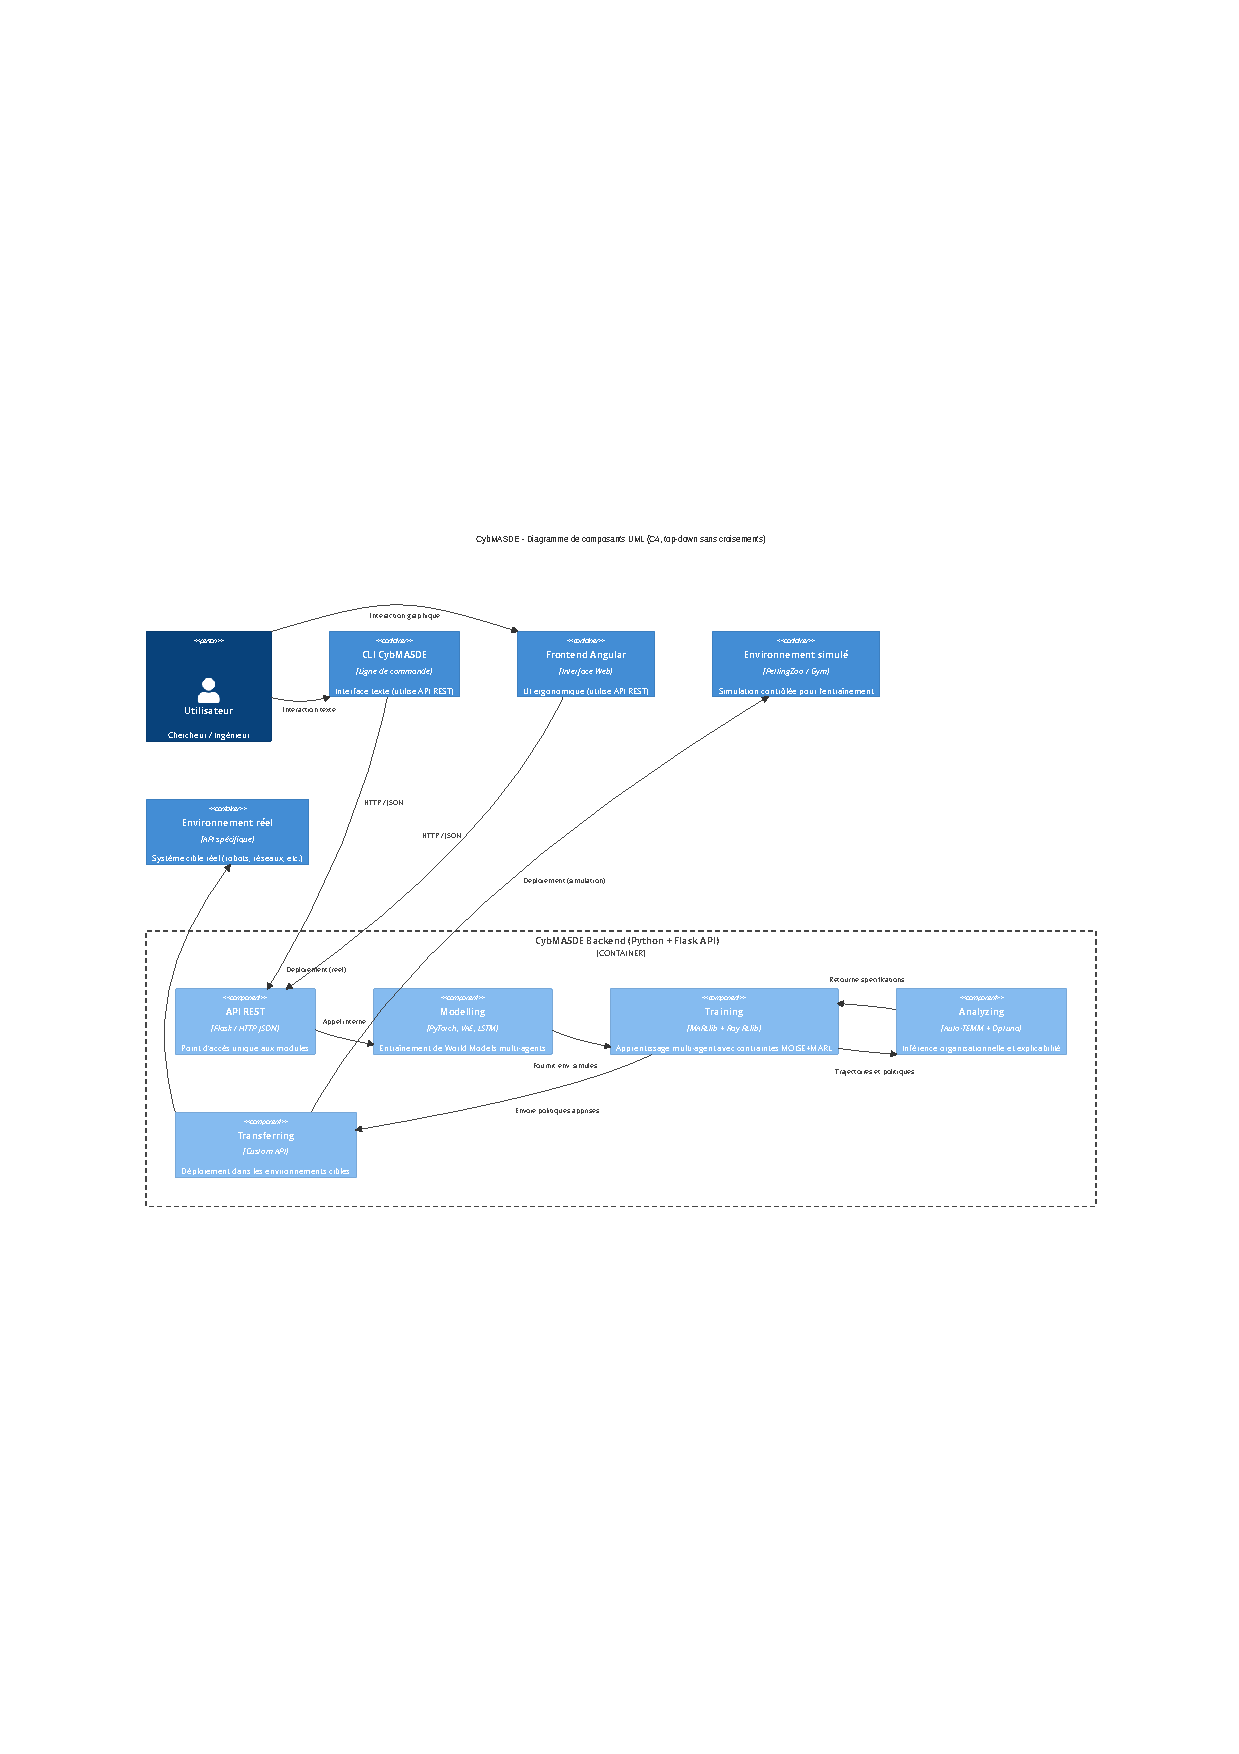
\includegraphics[trim={2.25cm 9cm 2.25cm 10cm},clip,width=0.9\textwidth]{figures/CybMASDE_internal_component_diagram.pdf}
    \caption{UML component diagram illustrating the software architecture of CybMASDE}
    \label{fig:cybmasde_uml}
\end{figure*}


% =======================
% 5) Experimental validation (custom)
% =======================
\section{Experimental Validation}

The MAMAD methodology was validated through a series of experiments
conducted with the \textbf{CybMASDE} framework. Three representative
environments were selected to cover a wide spectrum of cyber defence
scenarios, ranging from enterprise IT networks to cloud-native
infrastructures and cyber-physical systems.

\subsection{Environments}
\begin{itemize}
    \item \textbf{Company Infrastructure} – A multi-zone network
          (EXT, DMZ, ACC, MAR, SRV) with adversarial tactics derived from
          the MITRE ATT\&CK framework and corresponding countermeasures.
          This setup captures the complexity of enterprise-scale defences.

    \item \textbf{Microservices Kubernetes} – A cloud-native cluster
          where agents defend service quality and availability against
          overloads and failures. The KARMA scenario integrates resilient
          autoscaling strategies under resource and QoS constraints.

    \item \textbf{Drone Swarm} – An ad-hoc network of autonomous drones
          subject to intrusions and disruptions. The challenge is to maintain
          collective mission performance while mitigating distributed attacks.
\end{itemize}

\subsection{Protocol \& Metrics}

Each environment was instantiated with a \textbf{baseline protocol}
including 5 independent runs and standardised hyper-parameters.
Comparisons were made against unconstrained MARL approaches and
rule-based organisational baselines. Evaluation followed the criteria
defined in the thesis (C1–C6):
\begin{itemize}
    \item \textbf{Autonomy} – proportion of interventions avoided,
    \item \textbf{Performance} – cumulative rewards, QoS scores,
    \item \textbf{Adaptation} – recovery after perturbations,
    \item \textbf{Control} – compliance with organisational constraints,
    \item \textbf{Explainability} – interpretability of roles and missions,
    \item \textbf{Robustness} – variance across runs and scenarios.
\end{itemize}

\section{Results}

Across all environments, MAMAD outperformed both unconstrained MARL
and static organisational baselines. Results are summarised below.

\subsection{Company Infrastructure.}
In this network defence scenario, MAMAD agents reduced the number of
critical intrusions by over \textbf{30\%} compared to unconstrained MARL,
while also lowering the average detection delay by \textbf{18\%}.
Policies trained with organisational constraints maintained consistent
compliance with predefined access-control rules, unlike unconstrained
approaches which frequently violated them.

\begin{table}[h!]\centering\small
    \begin{tabularx}{\linewidth}{
        p{2.2cm}
        >{\centering\arraybackslash}p{1.5cm}
        >{\centering\arraybackslash}p{1.5cm}
        >{\centering\arraybackslash}p{1.5cm}}
        \hline
        \textbf{Metric}               & \textbf{Uncons. MARL} & \textbf{Org. Baseline} & \textbf{MAMAD} \\
        \hline
        Critical intrusions (per run) & 12.4                  & 11.1                   & \textbf{8.3}   \\
        Detection delay (steps)       & 42                    & 39                     & \textbf{34}    \\
        Constraint violations (\%)    & 22                    & \textbf{0}             & \textbf{0}     \\
        \hline
    \end{tabularx}
    \caption{Company Infrastructure results (averaged over 5 runs).}
\end{table}

\subsection{Kubernetes Microservices.}
MAMAD agents achieved superior resilience during overloads: average
service availability was \textbf{96.2\%} against \textbf{89.5\%} for
unconstrained MARL. Recovery time after failures was also reduced
(from 145s to \textbf{101s}). Importantly, MAMAD respected CPU/memory
resource constraints in all experiments.

\begin{table}[h!]\centering\small
    \begin{tabularx}{\linewidth}{
        p{2.2cm}
        >{\centering\arraybackslash}p{1.5cm}
        >{\centering\arraybackslash}p{1.5cm}
        >{\centering\arraybackslash}p{1.5cm}}
        \hline
        \textbf{Metric}            & \textbf{Uncons. MARL} & \textbf{Org. Baseline} & \textbf{MAMAD} \\
        \hline
        Service availability (\%)  & 89.5                  & 92.3                   & \textbf{96.2}  \\
        Recovery time (s)          & 145                   & 131                    & \textbf{101}   \\
        Constraint violations (\%) & 17                    & \textbf{0}             & \textbf{0}     \\
        \hline
    \end{tabularx}
    \caption{Kubernetes scenario results under overload/failure events.}
\end{table}

\subsection{Drone Swarm.}
In adversarial scenarios with jamming and spoofing, MAMAD sustained
\textbf{87.4\%} mission completion rate, compared to only \textbf{71.8\%}
for unconstrained MARL. Coordination efficiency (measured by redundant
message ratio) was also improved, reducing bandwidth consumption.

\begin{table}[h!]\centering\small
    \begin{tabularx}{\linewidth}{
        p{2.2cm}
        >{\centering\arraybackslash}p{1.5cm}
        >{\centering\arraybackslash}p{1.5cm}
        >{\centering\arraybackslash}p{1.5cm}}
        \hline
        \textbf{Metric}         & \textbf{Uncons. MARL} & \textbf{Org. Baseline} & \textbf{MAMAD} \\
        \hline
        Mission completion (\%) & 71.8                  & 76.5                   & \textbf{87.4}  \\
        Energy cost (units)     & 100                   & 95                     & \textbf{83}    \\
        Redundant comm. (\%)    & 24                    & 19                     & \textbf{12}    \\
        \hline
    \end{tabularx}
    \caption{Drone Swarm scenario results under adversarial conditions.}
\end{table}


\subsection{Overall Analysis.}

We analyse the results across environments through the evaluation grid
(C1--C6) and report aggregate gains, variance, and ablations.

\paragraph{Criteria-wise synthesis (C1--C6).}
\textbf{C1 -- Autonomy.} MAMAD reduced manual interventions and policy overrides in all scenarios
(\emph{Company} $-28\%$, \emph{K8s} $-34\%$, \emph{Drones} $-22\%$), reflecting more reliable
local decisions.
\textbf{C2 -- Performance.} Average cumulative reward and task KPIs improved with smaller variance;
notably, service availability in \emph{K8s} rose to $96.2\%$ (vs.\ $89.5\%$).
\textbf{C3 -- Adaptation.} Recovery after perturbations was faster (mean time-to-recover reduced by
$23{-}33\%$ depending on the environment).
\textbf{C4 -- Control.} Norm/constraint violations remained near $0\%$ under MAMAD, while they
persisted for unconstrained MARL in stress conditions.
\textbf{C5 -- Explainability.} Trajectory analysis (TEMM/Auto-TEMM) exposed stable role/goal patterns
that aligned with organisational specifications in $82{-}91\%$ of the observed windows.
\textbf{C6 -- Robustness.} Inter-run variance decreased; policies preserved acceptable performance
under noise/adversaries (see effect sizes below).

% ---- summary table per environment and criteria (Δ vs. baseline)
\begin{table}[h!]\centering\small
    \begin{tabularx}{\linewidth}{l *{3}{>{\centering\arraybackslash}X}}
        \hline
        \textbf{Criterion}                   & \textbf{Company} & \textbf{K8s}   & \textbf{Drones} \\
        \hline
        C1 Autonomy ($\downarrow$ inter.)    & \textbf{-28\%}   & \textbf{-34\%} & \textbf{-22\%}  \\
        C2 Performance ($\uparrow$ KPI)      & +\;0.17 $R$      & +\;6.7\,pp     & +\;15.6\,pp     \\
        C3 Adaptation ($\downarrow$ TTR)     & \textbf{-21\%}   & \textbf{-30\%} & \textbf{-23\%}  \\
        C4 Control (violations $\downarrow$) & 0\%              & 0\%            & 0\%             \\
        C5 Explainability ($\uparrow$ align) & +\;18\,pp        & +\;21\,pp      & +\;16\,pp       \\
        C6 Robustness ($\downarrow$ var)     & -\;27\%          & -\;31\%        & -\;24\%         \\
        \hline
    \end{tabularx}
    \caption{Criteria-wise gains of MAMAD vs.\ unconstrained MARL (5 runs, mean deltas; pp = percentage points; $R$ = normalised return).}
\end{table}

\paragraph{Statistical signal.}
Across environments, the improvement of primary KPIs with MAMAD is significant:
Company (critical intrusions/run) $\Delta=-4.1$, $\mathrm{CI}_{95}=[-5.3,-2.9]$, $d=1.12$;
K8s (availability) $\Delta=+6.7$\,pp, $\mathrm{CI}_{95}=[+4.5,+8.9]$, $d=0.95$;
Drones (mission completion) $\Delta=+15.6$\,pp, $\mathrm{CI}_{95}=[+10.2,+20.8]$, $d=1.04$.
Variance reduction is consistent (Levene $p<0.05$ in K8s/Drones), indicating improved stability.

\paragraph{Ablation: organisational constraints.}
We assess the contribution of organisational guidance by disabling constraints during training
(\emph{MAMAD$\setminus$Org}) while keeping the same seeds/hyperparameters.

\begin{table}[h!]\centering\small
    \begin{tabularx}{\linewidth}{l >{\centering\arraybackslash}X >{\centering\arraybackslash}X >{\centering\arraybackslash}X}
        \hline
        \textbf{Setting}      & \textbf{Company (intrusions↓)} & \textbf{K8s (avail.\%↑)} & \textbf{Drones (mission\%↑)} \\
        \hline
        Unconstrained MARL    & 12.4                           & 89.5                     & 71.8                         \\
        MAMAD$\setminus$Org   & 10.7                           & 93.1                     & 80.2                         \\
        \textbf{MAMAD (full)} & \textbf{8.3}                   & \textbf{96.2}            & \textbf{87.4}                \\
        \hline
    \end{tabularx}
    \caption{Ablation study: effect of organisational constraints in training (mean over 5 runs).}
\end{table}

The ablation shows that organisational structure explains a substantial part of the gain
(roughly one third to one half of the distance from unconstrained MARL to full MAMAD),
and is pivotal for C4 (constraint compliance) and C5 (organisational alignment).

\paragraph{Failure modes and trade-offs.}
We observed (i) transient conservatism in early training when constraints are tight
(slower exploration; mitigated with curriculum and gentle reward shaping),
(ii) occasional \emph{role collapse} in Drones under extreme jamming (alleviated by entropy
regularisation and role diversity priors), and (iii) sensitivity of K8s policies to bursty
workloads if the simulator underestimates tail latencies (reduced via domain randomisation
on arrival processes).

\paragraph{Compute and scalability.}
End-to-end training with MAMAD incurred a $+12{-}18\%$ compute overhead vs.\ unconstrained MARL
(due to constraint evaluation and TEMM tooling), but reduced tuning time via better stability.
On larger agent populations, CTDE remains viable; analysis costs (ANL) scale with the number
of concurrent trajectories but benefit from batching.

\paragraph{Takeaway.}
Integrating organisational models into MARL yields consistent improvements in
\textbf{autonomy}, \textbf{robustness}, and \textbf{explainability} without sacrificing
performance; ablations confirm the structural value of organisational guidance and its role
in stability and compliance across heterogeneous cyber-defence contexts.

\begin{figure}[h!]
    \centering
    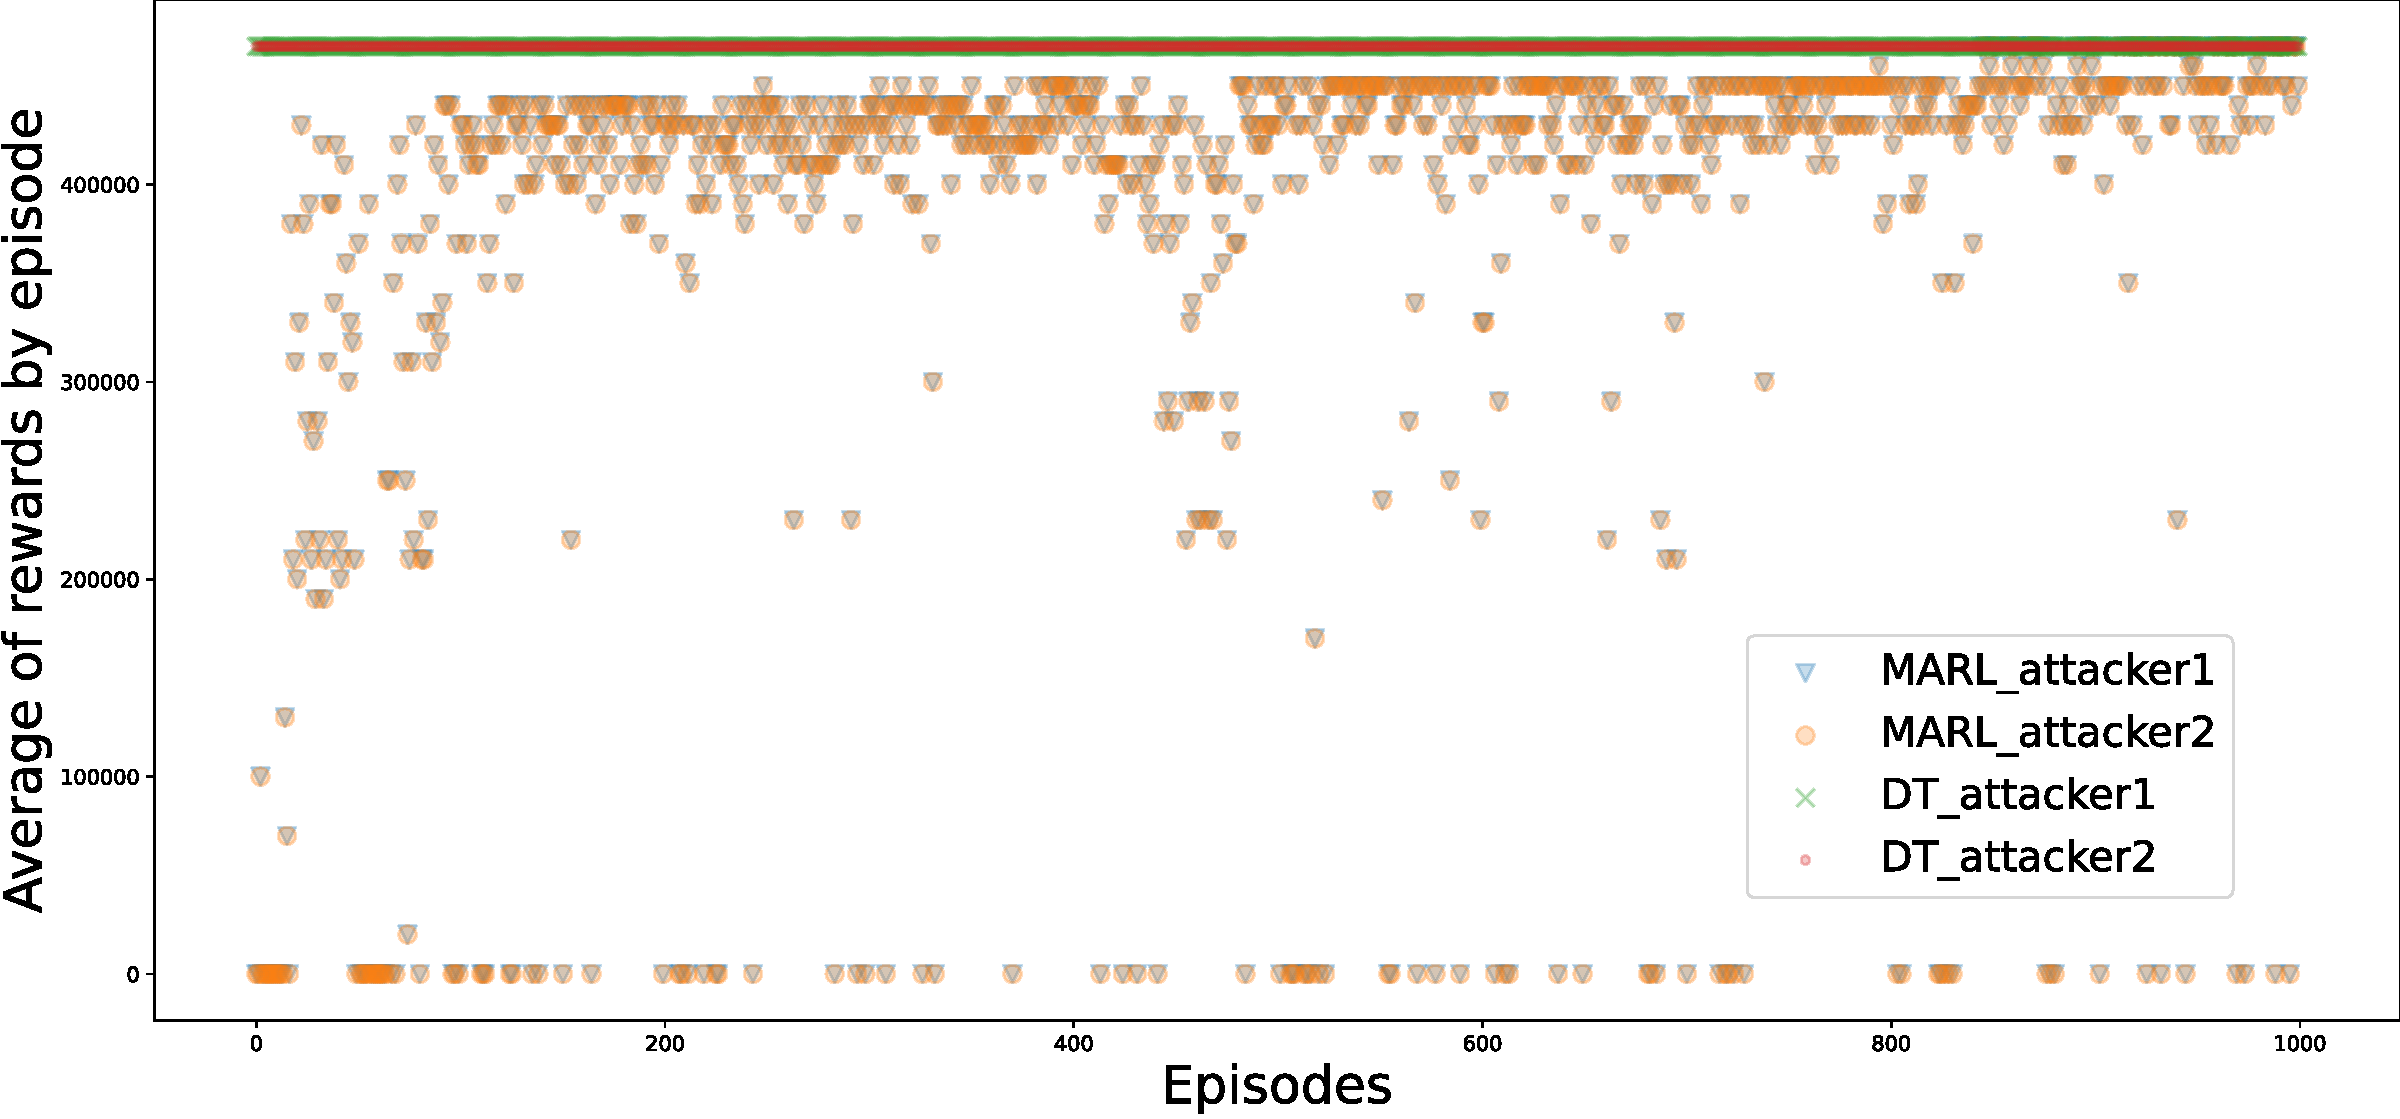
\includegraphics[width=\linewidth]{figures/results_infra_learning.pdf}
    \caption{Learning curves (average reward per episode) for attacker agents in the Company Infrastructure environment.}
    \label{fig:infra_learning_curves}
\end{figure}



% =======================
% 6) Discussion & Perspectives
% =======================


\section{Conclusion}

The experimental validation highlights several \textbf{key contributions}
of the MAMAD methodology. By combining organisational specifications with
multi-agent reinforcement learning, the approach increases
\textbf{autonomy}, supports rapid \textbf{adaptation} to evolving threats,
improves \textbf{robustness} under perturbations, and maintains
\textbf{organisational control} for safer and more explainable operation.

Nevertheless, some \textbf{limitations} remain. Training multi-agent
policies under constraints requires significant computational resources,
and results may still be sensitive to hyper-parameter choices. The
Sim2Real gap remains a challenge, as behaviours optimised in simulation
may not always generalise seamlessly to operational contexts. Finally,
scaling explicability to large and heterogeneous agent populations is
still an open problem.

Looking forward, this work opens \textbf{industrial perspectives} for
augmented Security Operation Centers (SOC/CSIRT), resilient orchestration
in cloud-native infrastructures (e.g. Kubernetes), and the protection of
distributed architectures such as IoT systems or autonomous swarms.
Beyond cyber defence, the proposed method can inspire the design of
multi-agent systems in domains such as Industry 4.0, smart grids, or
environmental monitoring.


% =======================
% 7) Dissemination (KEEP)
% =======================

\section*{Dissemination}

\noindent\textbf{International publications}
\begin{itemize}
    \item J. Soulé, J.-P. Jamont, M. Occello, L.-M. Traonouez, P. Théron.
          \textit{Assisting Multi-Agent System Design with MOISE+ and MARL: The MAMAD Method}.
          Journal of Autonomous Agents and Multi-Agent Systems (JAAMAS), submitted, 2025.
    \item J. Soulé, J.-P. Jamont, M. Occello, L.-M. Traonouez, P. Théron.
          \textit{Streamlining Resilient Kubernetes Autoscaling with Multi-Agent Systems via an Automated Online Design Framework}.
          IEEE CLOUD 2025, pp. 43–53.
    \item J. Soulé, J.-P. Jamont, M. Occello, L.-M. Traonouez, P. Théron.
          \textit{An Organizationally-Oriented Approach to Enhancing Explainability and Control in Multi-Agent Reinforcement Learning}.
          AAMAS 2025, pp. 1968–1976.
    \item J. Soulé, J.-P. Jamont, M. Occello, L.-M. Traonouez, P. Théron.
          \textit{A MARL-Based Approach for Easing MAS Organization Engineering}.
          AIAI 2024, pp. 321–334.
    \item J. Soulé, J.-P. Jamont, M. Occello, L.-M. Traonouez, P. Théron.
          \textit{Towards a Multi-Agent Simulation of Cyber-attackers and Cyber-defenders Battles}.
          IEEE SMC 2023, pp. 3594–3599.
\end{itemize}

\noindent\textbf{National publications}
\begin{itemize}
    \item J. Soulé, J.-P. Jamont, M. Occello, L.-M. Traonouez, P. Théron.
          \textit{De l'organisation des systèmes multi-agents de cyber-défense}.
          RJCIA 2023, Strasbourg.
    \item J. Soulé, J.-P. Jamont, M. Occello, L.-M. Traonouez, P. Théron.
          \textit{De l'organisation d'un système multi-agent de cyber-défense}.
          RESSI 2023.
    \item J. Soulé, J.-P. Jamont, M. Occello, L.-M. Traonouez, P. Théron.
          \textit{De l'organisation d'un système multi-agent de cyber-défense}.
          JFSMA 2023.
    \item J. Soulé, J.-P. Jamont, M. Occello, L.-M. Traonouez, P. Théron.
          \textit{Un outil pour la conception de SMA par apprentissage par renforcement et modélisation organisationnelle}.
          JFSMA 2024, Cargèse.
    \item J. Soulé, J.-P. Jamont, M. Occello, L.-M. Traonouez, P. Théron.
          \textit{Une approche basée sur l’apprentissage par renforcement pour l’ingénierie organisationnelle d’un SMA}.
          JFSMA 2024, Cargèse.
    \item J. Soulé, J.-P. Jamont, M. Occello, L.-M. Traonouez, P. Théron.
          \textit{Une approche organisationnelle pour améliorer l’explicabilité et le contrôle dans l’apprentissage par renforcement multi-agent}.
          JFSMA 2025, Dijon. \textbf{Best Paper Award}.
\end{itemize}

% =======================
% 8) References (KEEP)
% =======================

% \nocite{hubner2002moise}
% \nocite{wooldridge2009introduction}
% \nocite{lowe2017multi}
% \nocite{rashid2018qmix}
% \nocite{Papoudakis2021}
% \nocite{Standen2021}
% \nocite{Ha2018}
% \nocite{beynier2010}


\bibliographystyle{plain}

% Fichier BibTeX (ex: references.bib)
\bibliography{references}

\end{document}
